\documentclass[twoside]{book}

% Packages required by doxygen
\usepackage{calc}
\usepackage{doxygen}
\usepackage{graphicx}
\usepackage[utf8]{inputenc}
\usepackage{makeidx}
\usepackage{multicol}
\usepackage{multirow}
\usepackage{textcomp}
\usepackage[table]{xcolor}

% Font selection
\usepackage[T1]{fontenc}
\usepackage{mathptmx}
\usepackage[scaled=.90]{helvet}
\usepackage{courier}
\usepackage{amssymb}
\usepackage{sectsty}
\renewcommand{\familydefault}{\sfdefault}
\allsectionsfont{%
  \fontseries{bc}\selectfont%
  \color{darkgray}%
}
\renewcommand{\DoxyLabelFont}{%
  \fontseries{bc}\selectfont%
  \color{darkgray}%
}

% Page & text layout
\usepackage{geometry}
\geometry{%
  a4paper,%
  top=2.5cm,%
  bottom=2.5cm,%
  left=2.5cm,%
  right=2.5cm%
}
\tolerance=750
\hfuzz=15pt
\hbadness=750
\setlength{\emergencystretch}{15pt}
\setlength{\parindent}{0cm}
\setlength{\parskip}{0.2cm}
\makeatletter
\renewcommand{\paragraph}{%
  \@startsection{paragraph}{4}{0ex}{-1.0ex}{1.0ex}{%
    \normalfont\normalsize\bfseries\SS@parafont%
  }%
}
\renewcommand{\subparagraph}{%
  \@startsection{subparagraph}{5}{0ex}{-1.0ex}{1.0ex}{%
    \normalfont\normalsize\bfseries\SS@subparafont%
  }%
}
\makeatother

% Headers & footers
\usepackage{fancyhdr}
\pagestyle{fancyplain}
\fancyhead[LE]{\fancyplain{}{\bfseries\thepage}}
\fancyhead[CE]{\fancyplain{}{}}
\fancyhead[RE]{\fancyplain{}{\bfseries\leftmark}}
\fancyhead[LO]{\fancyplain{}{\bfseries\rightmark}}
\fancyhead[CO]{\fancyplain{}{}}
\fancyhead[RO]{\fancyplain{}{\bfseries\thepage}}
\fancyfoot[LE]{\fancyplain{}{}}
\fancyfoot[CE]{\fancyplain{}{}}
\fancyfoot[RE]{\fancyplain{}{\bfseries\scriptsize Generated on Mon Jul 13 2015 16\-:20\-:46 for My Project by Doxygen }}
\fancyfoot[LO]{\fancyplain{}{\bfseries\scriptsize Generated on Mon Jul 13 2015 16\-:20\-:46 for My Project by Doxygen }}
\fancyfoot[CO]{\fancyplain{}{}}
\fancyfoot[RO]{\fancyplain{}{}}
\renewcommand{\footrulewidth}{0.4pt}
\renewcommand{\chaptermark}[1]{%
  \markboth{#1}{}%
}
\renewcommand{\sectionmark}[1]{%
  \markright{\thesection\ #1}%
}

% Indices & bibliography
\usepackage{natbib}
\usepackage[titles]{tocloft}
\setcounter{tocdepth}{3}
\setcounter{secnumdepth}{5}
\makeindex

% Hyperlinks (required, but should be loaded last)
\usepackage{ifpdf}
\ifpdf
  \usepackage[pdftex,pagebackref=true]{hyperref}
\else
  \usepackage[ps2pdf,pagebackref=true]{hyperref}
\fi
\hypersetup{%
  colorlinks=true,%
  linkcolor=blue,%
  citecolor=blue,%
  unicode%
}

% Custom commands
\newcommand{\clearemptydoublepage}{%
  \newpage{\pagestyle{empty}\cleardoublepage}%
}


%===== C O N T E N T S =====

\begin{document}

% Titlepage & ToC
\hypersetup{pageanchor=false}
\pagenumbering{roman}
\begin{titlepage}
\vspace*{7cm}
\begin{center}%
{\Large My Project }\\
\vspace*{1cm}
{\large Generated by Doxygen 1.8.6}\\
\vspace*{0.5cm}
{\small Mon Jul 13 2015 16:20:46}\\
\end{center}
\end{titlepage}
\clearemptydoublepage
\tableofcontents
\clearemptydoublepage
\pagenumbering{arabic}
\hypersetup{pageanchor=true}

%--- Begin generated contents ---
\chapter{Namespace Index}
\section{Namespace List}
Here is a list of all namespaces with brief descriptions\-:\begin{DoxyCompactList}
\item\contentsline{section}{\hyperlink{namespaceUi}{Ui} }{\pageref{namespaceUi}}{}
\end{DoxyCompactList}

\chapter{Hierarchical Index}
\section{Class Hierarchy}
This inheritance list is sorted roughly, but not completely, alphabetically\-:\begin{DoxyCompactList}
\item \contentsline{section}{Feld}{\pageref{classFeld}}{}
\item Q\-G\-L\-Widget\begin{DoxyCompactList}
\item \contentsline{section}{G\-L\-Widget}{\pageref{classGLWidget}}{}
\end{DoxyCompactList}
\item Q\-Main\-Window\begin{DoxyCompactList}
\item \contentsline{section}{Main\-Window}{\pageref{classMainWindow}}{}
\end{DoxyCompactList}
\item Q\-Object\begin{DoxyCompactList}
\item \contentsline{section}{Reversi}{\pageref{classReversi}}{}
\end{DoxyCompactList}
\item Q\-Widget\begin{DoxyCompactList}
\item \contentsline{section}{Credits}{\pageref{classCredits}}{}
\item \contentsline{section}{gewinner}{\pageref{classgewinner}}{}
\item \contentsline{section}{Hauptmenue}{\pageref{classHauptmenue}}{}
\item \contentsline{section}{new\-Game}{\pageref{classnewGame}}{}
\item \contentsline{section}{Open\-G\-L\-Game}{\pageref{classOpenGLGame}}{}
\item \contentsline{section}{Spiel\-Laden}{\pageref{classSpielLaden}}{}
\end{DoxyCompactList}
\item \contentsline{section}{Spielbrett}{\pageref{classSpielbrett}}{}
\item \contentsline{section}{Spieler}{\pageref{classSpieler}}{}
\item \contentsline{section}{Spielzug}{\pageref{classSpielzug}}{}
\item \contentsline{section}{Spielzug\-Liste}{\pageref{classSpielzugListe}}{}
\item \contentsline{section}{Ui\-\_\-\-Credits}{\pageref{classUi__Credits}}{}
\begin{DoxyCompactList}
\item \contentsline{section}{Ui\-:\-:Credits}{\pageref{classUi_1_1Credits}}{}
\end{DoxyCompactList}
\item \contentsline{section}{Ui\-\_\-gewinner}{\pageref{classUi__gewinner}}{}
\begin{DoxyCompactList}
\item \contentsline{section}{Ui\-:\-:gewinner}{\pageref{classUi_1_1gewinner}}{}
\end{DoxyCompactList}
\item \contentsline{section}{Ui\-\_\-\-Hauptmenue}{\pageref{classUi__Hauptmenue}}{}
\begin{DoxyCompactList}
\item \contentsline{section}{Ui\-:\-:Hauptmenue}{\pageref{classUi_1_1Hauptmenue}}{}
\end{DoxyCompactList}
\item \contentsline{section}{Ui\-\_\-\-Main\-Window}{\pageref{classUi__MainWindow}}{}
\begin{DoxyCompactList}
\item \contentsline{section}{Ui\-:\-:Main\-Window}{\pageref{classUi_1_1MainWindow}}{}
\end{DoxyCompactList}
\item \contentsline{section}{Ui\-\_\-new\-Game}{\pageref{classUi__newGame}}{}
\begin{DoxyCompactList}
\item \contentsline{section}{Ui\-:\-:new\-Game}{\pageref{classUi_1_1newGame}}{}
\end{DoxyCompactList}
\item \contentsline{section}{Ui\-\_\-\-Open\-G\-L\-Game}{\pageref{classUi__OpenGLGame}}{}
\begin{DoxyCompactList}
\item \contentsline{section}{Ui\-:\-:Open\-G\-L\-Game}{\pageref{classUi_1_1OpenGLGame}}{}
\end{DoxyCompactList}
\item \contentsline{section}{Ui\-\_\-\-Spiel\-Laden}{\pageref{classUi__SpielLaden}}{}
\begin{DoxyCompactList}
\item \contentsline{section}{Ui\-:\-:Spiel\-Laden}{\pageref{classUi_1_1SpielLaden}}{}
\end{DoxyCompactList}
\end{DoxyCompactList}

\chapter{Class Index}
\section{Class List}
Here are the classes, structs, unions and interfaces with brief descriptions\-:\begin{DoxyCompactList}
\item\contentsline{section}{\hyperlink{classCredits}{Credits} }{\pageref{classCredits}}{}
\item\contentsline{section}{\hyperlink{classUi_1_1Credits}{Ui\-::\-Credits} }{\pageref{classUi_1_1Credits}}{}
\item\contentsline{section}{\hyperlink{classFeld}{Feld} }{\pageref{classFeld}}{}
\item\contentsline{section}{\hyperlink{classUi_1_1gewinner}{Ui\-::gewinner} }{\pageref{classUi_1_1gewinner}}{}
\item\contentsline{section}{\hyperlink{classgewinner}{gewinner} }{\pageref{classgewinner}}{}
\item\contentsline{section}{\hyperlink{classGLWidget}{G\-L\-Widget} }{\pageref{classGLWidget}}{}
\item\contentsline{section}{\hyperlink{classHauptmenue}{Hauptmenue} }{\pageref{classHauptmenue}}{}
\item\contentsline{section}{\hyperlink{classUi_1_1Hauptmenue}{Ui\-::\-Hauptmenue} }{\pageref{classUi_1_1Hauptmenue}}{}
\item\contentsline{section}{\hyperlink{classUi_1_1MainWindow}{Ui\-::\-Main\-Window} }{\pageref{classUi_1_1MainWindow}}{}
\item\contentsline{section}{\hyperlink{classMainWindow}{Main\-Window} }{\pageref{classMainWindow}}{}
\item\contentsline{section}{\hyperlink{classUi_1_1newGame}{Ui\-::new\-Game} }{\pageref{classUi_1_1newGame}}{}
\item\contentsline{section}{\hyperlink{classnewGame}{new\-Game} }{\pageref{classnewGame}}{}
\item\contentsline{section}{\hyperlink{classOpenGLGame}{Open\-G\-L\-Game} }{\pageref{classOpenGLGame}}{}
\item\contentsline{section}{\hyperlink{classUi_1_1OpenGLGame}{Ui\-::\-Open\-G\-L\-Game} }{\pageref{classUi_1_1OpenGLGame}}{}
\item\contentsline{section}{\hyperlink{classReversi}{Reversi} }{\pageref{classReversi}}{}
\item\contentsline{section}{\hyperlink{classSpielbrett}{Spielbrett} }{\pageref{classSpielbrett}}{}
\item\contentsline{section}{\hyperlink{classSpieler}{Spieler} }{\pageref{classSpieler}}{}
\item\contentsline{section}{\hyperlink{classUi_1_1SpielLaden}{Ui\-::\-Spiel\-Laden} }{\pageref{classUi_1_1SpielLaden}}{}
\item\contentsline{section}{\hyperlink{classSpielLaden}{Spiel\-Laden} }{\pageref{classSpielLaden}}{}
\item\contentsline{section}{\hyperlink{classSpielzug}{Spielzug} }{\pageref{classSpielzug}}{}
\item\contentsline{section}{\hyperlink{classSpielzugListe}{Spielzug\-Liste} }{\pageref{classSpielzugListe}}{}
\item\contentsline{section}{\hyperlink{classUi__Credits}{Ui\-\_\-\-Credits} }{\pageref{classUi__Credits}}{}
\item\contentsline{section}{\hyperlink{classUi__gewinner}{Ui\-\_\-gewinner} }{\pageref{classUi__gewinner}}{}
\item\contentsline{section}{\hyperlink{classUi__Hauptmenue}{Ui\-\_\-\-Hauptmenue} }{\pageref{classUi__Hauptmenue}}{}
\item\contentsline{section}{\hyperlink{classUi__MainWindow}{Ui\-\_\-\-Main\-Window} }{\pageref{classUi__MainWindow}}{}
\item\contentsline{section}{\hyperlink{classUi__newGame}{Ui\-\_\-new\-Game} }{\pageref{classUi__newGame}}{}
\item\contentsline{section}{\hyperlink{classUi__OpenGLGame}{Ui\-\_\-\-Open\-G\-L\-Game} }{\pageref{classUi__OpenGLGame}}{}
\item\contentsline{section}{\hyperlink{classUi__SpielLaden}{Ui\-\_\-\-Spiel\-Laden} }{\pageref{classUi__SpielLaden}}{}
\end{DoxyCompactList}

\chapter{File Index}
\section{File List}
Here is a list of all files with brief descriptions\-:\begin{DoxyCompactList}
\item\contentsline{section}{\hyperlink{credits_8cpp}{credits.\-cpp} }{\pageref{credits_8cpp}}{}
\item\contentsline{section}{\hyperlink{credits_8h}{credits.\-h} }{\pageref{credits_8h}}{}
\item\contentsline{section}{\hyperlink{DEFINE_8h}{D\-E\-F\-I\-N\-E.\-h} }{\pageref{DEFINE_8h}}{}
\item\contentsline{section}{\hyperlink{feld_8cpp}{feld.\-cpp} }{\pageref{feld_8cpp}}{}
\item\contentsline{section}{\hyperlink{feld_8h}{feld.\-h} }{\pageref{feld_8h}}{}
\item\contentsline{section}{\hyperlink{gewinner_8cpp}{gewinner.\-cpp} }{\pageref{gewinner_8cpp}}{}
\item\contentsline{section}{\hyperlink{gewinner_8h}{gewinner.\-h} }{\pageref{gewinner_8h}}{}
\item\contentsline{section}{\hyperlink{glwidget_8cpp}{glwidget.\-cpp} }{\pageref{glwidget_8cpp}}{}
\item\contentsline{section}{\hyperlink{glwidget_8h}{glwidget.\-h} }{\pageref{glwidget_8h}}{}
\item\contentsline{section}{\hyperlink{hauptmenue_8cpp}{hauptmenue.\-cpp} }{\pageref{hauptmenue_8cpp}}{}
\item\contentsline{section}{\hyperlink{hauptmenue_8h}{hauptmenue.\-h} }{\pageref{hauptmenue_8h}}{}
\item\contentsline{section}{\hyperlink{loadshaders_8h}{loadshaders.\-h} }{\pageref{loadshaders_8h}}{}
\item\contentsline{section}{\hyperlink{main_8cpp}{main.\-cpp} }{\pageref{main_8cpp}}{}
\item\contentsline{section}{\hyperlink{mainwindow_8cpp}{mainwindow.\-cpp} }{\pageref{mainwindow_8cpp}}{}
\item\contentsline{section}{\hyperlink{mainwindow_8h}{mainwindow.\-h} }{\pageref{mainwindow_8h}}{}
\item\contentsline{section}{\hyperlink{newgame_8cpp}{newgame.\-cpp} }{\pageref{newgame_8cpp}}{}
\item\contentsline{section}{\hyperlink{newgame_8h}{newgame.\-h} }{\pageref{newgame_8h}}{}
\item\contentsline{section}{\hyperlink{openglgame_8cpp}{openglgame.\-cpp} }{\pageref{openglgame_8cpp}}{}
\item\contentsline{section}{\hyperlink{openglgame_8h}{openglgame.\-h} }{\pageref{openglgame_8h}}{}
\item\contentsline{section}{\hyperlink{reversi_8cpp}{reversi.\-cpp} }{\pageref{reversi_8cpp}}{}
\item\contentsline{section}{\hyperlink{reversi_8h}{reversi.\-h} }{\pageref{reversi_8h}}{}
\item\contentsline{section}{\hyperlink{spielbrett_8cpp}{spielbrett.\-cpp} }{\pageref{spielbrett_8cpp}}{}
\item\contentsline{section}{\hyperlink{spielbrett_8h}{spielbrett.\-h} }{\pageref{spielbrett_8h}}{}
\item\contentsline{section}{\hyperlink{spieler_8cpp}{spieler.\-cpp} }{\pageref{spieler_8cpp}}{}
\item\contentsline{section}{\hyperlink{spieler_8h}{spieler.\-h} }{\pageref{spieler_8h}}{}
\item\contentsline{section}{\hyperlink{spielladen_8cpp}{spielladen.\-cpp} }{\pageref{spielladen_8cpp}}{}
\item\contentsline{section}{\hyperlink{spielladen_8h}{spielladen.\-h} }{\pageref{spielladen_8h}}{}
\item\contentsline{section}{\hyperlink{spielzug_8cpp}{spielzug.\-cpp} }{\pageref{spielzug_8cpp}}{}
\item\contentsline{section}{\hyperlink{spielzug_8h}{spielzug.\-h} }{\pageref{spielzug_8h}}{}
\item\contentsline{section}{\hyperlink{spielzugliste_8cpp}{spielzugliste.\-cpp} }{\pageref{spielzugliste_8cpp}}{}
\item\contentsline{section}{\hyperlink{spielzugliste_8h}{spielzugliste.\-h} }{\pageref{spielzugliste_8h}}{}
\item\contentsline{section}{\hyperlink{ui__credits_8h}{ui\-\_\-credits.\-h} }{\pageref{ui__credits_8h}}{}
\item\contentsline{section}{\hyperlink{ui__gewinner_8h}{ui\-\_\-gewinner.\-h} }{\pageref{ui__gewinner_8h}}{}
\item\contentsline{section}{\hyperlink{ui__hauptmenue_8h}{ui\-\_\-hauptmenue.\-h} }{\pageref{ui__hauptmenue_8h}}{}
\item\contentsline{section}{\hyperlink{ui__mainwindow_8h}{ui\-\_\-mainwindow.\-h} }{\pageref{ui__mainwindow_8h}}{}
\item\contentsline{section}{\hyperlink{ui__newgame_8h}{ui\-\_\-newgame.\-h} }{\pageref{ui__newgame_8h}}{}
\item\contentsline{section}{\hyperlink{ui__openglgame_8h}{ui\-\_\-openglgame.\-h} }{\pageref{ui__openglgame_8h}}{}
\item\contentsline{section}{\hyperlink{ui__spielladen_8h}{ui\-\_\-spielladen.\-h} }{\pageref{ui__spielladen_8h}}{}
\end{DoxyCompactList}

\chapter{Namespace Documentation}
\hypertarget{namespaceUi}{\section{Ui Namespace Reference}
\label{namespaceUi}\index{Ui@{Ui}}
}
\subsection*{Classes}
\begin{DoxyCompactItemize}
\item 
class \hyperlink{classUi_1_1Credits}{Credits}
\item 
class \hyperlink{classUi_1_1gewinner}{gewinner}
\item 
class \hyperlink{classUi_1_1Hauptmenue}{Hauptmenue}
\item 
class \hyperlink{classUi_1_1MainWindow}{Main\-Window}
\item 
class \hyperlink{classUi_1_1newGame}{new\-Game}
\item 
class \hyperlink{classUi_1_1OpenGLGame}{Open\-G\-L\-Game}
\item 
class \hyperlink{classUi_1_1SpielLaden}{Spiel\-Laden}
\end{DoxyCompactItemize}

\chapter{Class Documentation}
\hypertarget{classCredits}{\section{Credits Class Reference}
\label{classCredits}\index{Credits@{Credits}}
}


{\ttfamily \#include $<$credits.\-h$>$}



Inheritance diagram for Credits\-:\nopagebreak
\begin{figure}[H]
\begin{center}
\leavevmode
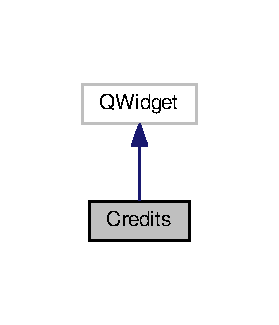
\includegraphics[width=134pt]{classCredits__inherit__graph}
\end{center}
\end{figure}


Collaboration diagram for Credits\-:\nopagebreak
\begin{figure}[H]
\begin{center}
\leavevmode
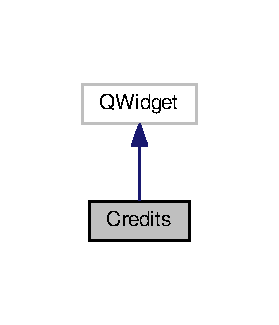
\includegraphics[width=134pt]{classCredits__coll__graph}
\end{center}
\end{figure}
\subsection*{Public Member Functions}
\begin{DoxyCompactItemize}
\item 
\hyperlink{classCredits_a68cb1b04910e4b3379637b9ece1d9040}{Credits} (Q\-Widget $\ast$parent=0, Q\-Stacked\-Widget $\ast$the\-Sites=0)
\item 
\hyperlink{classCredits_ad8ade10d61b682e4c4da83f2ede60792}{$\sim$\-Credits} ()
\end{DoxyCompactItemize}


\subsection{Detailed Description}
Das Credit-\/\-Widget hat die Funktion zum anzeigen der Programminformationen. 

\subsection{Constructor \& Destructor Documentation}
\hypertarget{classCredits_a68cb1b04910e4b3379637b9ece1d9040}{\index{Credits@{Credits}!Credits@{Credits}}
\index{Credits@{Credits}!Credits@{Credits}}
\subsubsection[{Credits}]{\setlength{\rightskip}{0pt plus 5cm}Credits\-::\-Credits (
\begin{DoxyParamCaption}
\item[{Q\-Widget $\ast$}]{parent = {\ttfamily 0}, }
\item[{Q\-Stacked\-Widget $\ast$}]{the\-Sites = {\ttfamily 0}}
\end{DoxyParamCaption}
)\hspace{0.3cm}{\ttfamily [explicit]}}}\label{classCredits_a68cb1b04910e4b3379637b9ece1d9040}
Konstruiert das Credits-\/\-Widget.


\begin{DoxyParams}{Parameters}
{\em parent} & Die Angabe des Eltern-\/\-Widgets. \\
\hline
{\em the\-Sites} & Die Angabe der zu erreichenden Widgets. \\
\hline
\end{DoxyParams}


Here is the call graph for this function\-:\nopagebreak
\begin{figure}[H]
\begin{center}
\leavevmode
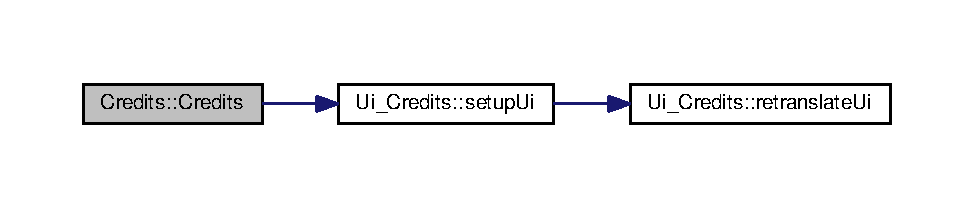
\includegraphics[width=350pt]{classCredits_a68cb1b04910e4b3379637b9ece1d9040_cgraph}
\end{center}
\end{figure}


\hypertarget{classCredits_ad8ade10d61b682e4c4da83f2ede60792}{\index{Credits@{Credits}!$\sim$\-Credits@{$\sim$\-Credits}}
\index{$\sim$\-Credits@{$\sim$\-Credits}!Credits@{Credits}}
\subsubsection[{$\sim$\-Credits}]{\setlength{\rightskip}{0pt plus 5cm}Credits\-::$\sim$\-Credits (
\begin{DoxyParamCaption}
{}
\end{DoxyParamCaption}
)}}\label{classCredits_ad8ade10d61b682e4c4da83f2ede60792}
Destruktor des Credits-\/\-Widgets. 

The documentation for this class was generated from the following files\-:\begin{DoxyCompactItemize}
\item 
\hyperlink{credits_8h}{credits.\-h}\item 
\hyperlink{credits_8cpp}{credits.\-cpp}\end{DoxyCompactItemize}

\hypertarget{classUi_1_1Credits}{\section{Ui\-:\-:Credits Class Reference}
\label{classUi_1_1Credits}\index{Ui\-::\-Credits@{Ui\-::\-Credits}}
}


{\ttfamily \#include $<$ui\-\_\-credits.\-h$>$}



Inheritance diagram for Ui\-:\-:Credits\-:\nopagebreak
\begin{figure}[H]
\begin{center}
\leavevmode
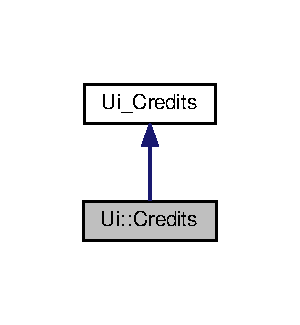
\includegraphics[width=144pt]{classUi_1_1Credits__inherit__graph}
\end{center}
\end{figure}


Collaboration diagram for Ui\-:\-:Credits\-:\nopagebreak
\begin{figure}[H]
\begin{center}
\leavevmode
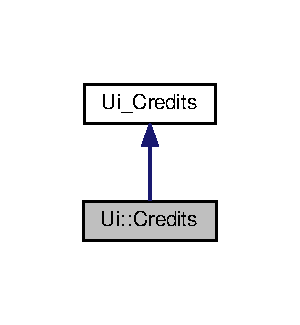
\includegraphics[width=144pt]{classUi_1_1Credits__coll__graph}
\end{center}
\end{figure}
\subsection*{Additional Inherited Members}


The documentation for this class was generated from the following file\-:\begin{DoxyCompactItemize}
\item 
\hyperlink{ui__credits_8h}{ui\-\_\-credits.\-h}\end{DoxyCompactItemize}

\hypertarget{classFeld}{\section{Feld Class Reference}
\label{classFeld}\index{Feld@{Feld}}
}


{\ttfamily \#include $<$feld.\-h$>$}

\subsection*{Public Member Functions}
\begin{DoxyCompactItemize}
\item 
\hyperlink{classFeld_a8a3098df53c8ae2ef988d0d2e34be1db}{Feld} ()
\item 
\hyperlink{DEFINE_8h_a38d3a135c8443ff29d22fa0756476c5b}{Feld\-Eigenschaft} \hyperlink{classFeld_a99a02b1d81eccc5ced54da45d37eedd1}{liefere\-Feldeigenschaft} ()
\item 
\hyperlink{DEFINE_8h_af7777a498318335ea89b85bdc0d1651f}{Spieler\-Farbe} \hyperlink{classFeld_a71857da4dc18318fc85c3332179db0a0}{liefere\-Farbe} ()
\item 
bool \hyperlink{classFeld_add4df21f3360a4405076f9e78f64c34e}{liefere\-Drehung} ()
\item 
void \hyperlink{classFeld_ae11f5df6990d6153f5c09f6e3f1d60d3}{aendere\-Eigenschaft} (\hyperlink{DEFINE_8h_a38d3a135c8443ff29d22fa0756476c5b}{Feld\-Eigenschaft} neue\-Eigenschaft)
\item 
void \hyperlink{classFeld_a214e1a88b71ffee9fb88c1643ec97525}{aendere\-Farbe} (\hyperlink{DEFINE_8h_af7777a498318335ea89b85bdc0d1651f}{Spieler\-Farbe} neue\-Farbe)
\item 
void \hyperlink{classFeld_a5668abf4e68ad86c820238a06a3ae2fd}{aendere\-Drehung} (bool drehen)
\item 
void \hyperlink{classFeld_a17f0cf8213cc7c98f3e8d73c9ed8bca9}{aendere\-Farbe\-Und\-Eigenschaft} (\hyperlink{DEFINE_8h_af7777a498318335ea89b85bdc0d1651f}{Spieler\-Farbe} neue\-Farbe, \hyperlink{DEFINE_8h_a38d3a135c8443ff29d22fa0756476c5b}{Feld\-Eigenschaft} neue\-Eigenschaft)
\end{DoxyCompactItemize}


\subsection{Detailed Description}
Diese Klasse repraesentiert ein \hyperlink{classFeld}{Feld} auf einem \hyperlink{classSpielbrett}{Spielbrett}. 

\subsection{Constructor \& Destructor Documentation}
\hypertarget{classFeld_a8a3098df53c8ae2ef988d0d2e34be1db}{\index{Feld@{Feld}!Feld@{Feld}}
\index{Feld@{Feld}!Feld@{Feld}}
\subsubsection[{Feld}]{\setlength{\rightskip}{0pt plus 5cm}Feld\-::\-Feld (
\begin{DoxyParamCaption}
{}
\end{DoxyParamCaption}
)}}\label{classFeld_a8a3098df53c8ae2ef988d0d2e34be1db}
Konstruiert ein Objekt vom Typ \hyperlink{classFeld}{Feld}, als leeres \hyperlink{classFeld}{Feld}, ohne drehung und mit der Spielerfarbe weiss. 

\subsection{Member Function Documentation}
\hypertarget{classFeld_a5668abf4e68ad86c820238a06a3ae2fd}{\index{Feld@{Feld}!aendere\-Drehung@{aendere\-Drehung}}
\index{aendere\-Drehung@{aendere\-Drehung}!Feld@{Feld}}
\subsubsection[{aendere\-Drehung}]{\setlength{\rightskip}{0pt plus 5cm}void Feld\-::aendere\-Drehung (
\begin{DoxyParamCaption}
\item[{bool}]{drehen}
\end{DoxyParamCaption}
)}}\label{classFeld_a5668abf4e68ad86c820238a06a3ae2fd}
Aendert die Drehung.


\begin{DoxyParams}{Parameters}
{\em drehen} & (True $\vert$ False) \\
\hline
\end{DoxyParams}
\hypertarget{classFeld_ae11f5df6990d6153f5c09f6e3f1d60d3}{\index{Feld@{Feld}!aendere\-Eigenschaft@{aendere\-Eigenschaft}}
\index{aendere\-Eigenschaft@{aendere\-Eigenschaft}!Feld@{Feld}}
\subsubsection[{aendere\-Eigenschaft}]{\setlength{\rightskip}{0pt plus 5cm}void Feld\-::aendere\-Eigenschaft (
\begin{DoxyParamCaption}
\item[{{\bf Feld\-Eigenschaft}}]{neue\-Eigenschaft}
\end{DoxyParamCaption}
)}}\label{classFeld_ae11f5df6990d6153f5c09f6e3f1d60d3}
Aendert die Feldeigenschaft.


\begin{DoxyParams}{Parameters}
{\em neue\-Eigenschaft} & Die neue Feld\-Eigenschaft. \\
\hline
\end{DoxyParams}
\hypertarget{classFeld_a214e1a88b71ffee9fb88c1643ec97525}{\index{Feld@{Feld}!aendere\-Farbe@{aendere\-Farbe}}
\index{aendere\-Farbe@{aendere\-Farbe}!Feld@{Feld}}
\subsubsection[{aendere\-Farbe}]{\setlength{\rightskip}{0pt plus 5cm}void Feld\-::aendere\-Farbe (
\begin{DoxyParamCaption}
\item[{{\bf Spieler\-Farbe}}]{neue\-Farbe}
\end{DoxyParamCaption}
)}}\label{classFeld_a214e1a88b71ffee9fb88c1643ec97525}
Aendert die Farbe.


\begin{DoxyParams}{Parameters}
{\em neue\-Farbe} & Die neue Farbe. \\
\hline
\end{DoxyParams}
\hypertarget{classFeld_a17f0cf8213cc7c98f3e8d73c9ed8bca9}{\index{Feld@{Feld}!aendere\-Farbe\-Und\-Eigenschaft@{aendere\-Farbe\-Und\-Eigenschaft}}
\index{aendere\-Farbe\-Und\-Eigenschaft@{aendere\-Farbe\-Und\-Eigenschaft}!Feld@{Feld}}
\subsubsection[{aendere\-Farbe\-Und\-Eigenschaft}]{\setlength{\rightskip}{0pt plus 5cm}void Feld\-::aendere\-Farbe\-Und\-Eigenschaft (
\begin{DoxyParamCaption}
\item[{{\bf Spieler\-Farbe}}]{neue\-Farbe, }
\item[{{\bf Feld\-Eigenschaft}}]{neue\-Eigenschaft}
\end{DoxyParamCaption}
)}}\label{classFeld_a17f0cf8213cc7c98f3e8d73c9ed8bca9}
Aendert sowohl die Feldeigenschaft, als auch die Farbe des Feldes.


\begin{DoxyParams}{Parameters}
{\em neue\-Farbe} & Die neue Farbe. \\
\hline
{\em neue\-Eigenschaft} & Die neue Feldeigenschaft. \\
\hline
\end{DoxyParams}
\hypertarget{classFeld_add4df21f3360a4405076f9e78f64c34e}{\index{Feld@{Feld}!liefere\-Drehung@{liefere\-Drehung}}
\index{liefere\-Drehung@{liefere\-Drehung}!Feld@{Feld}}
\subsubsection[{liefere\-Drehung}]{\setlength{\rightskip}{0pt plus 5cm}bool Feld\-::liefere\-Drehung (
\begin{DoxyParamCaption}
{}
\end{DoxyParamCaption}
)}}\label{classFeld_add4df21f3360a4405076f9e78f64c34e}
Liefert die Drehung (true $\vert$ false).

\begin{DoxyReturn}{Returns}
Die Drehung. 
\end{DoxyReturn}
\hypertarget{classFeld_a71857da4dc18318fc85c3332179db0a0}{\index{Feld@{Feld}!liefere\-Farbe@{liefere\-Farbe}}
\index{liefere\-Farbe@{liefere\-Farbe}!Feld@{Feld}}
\subsubsection[{liefere\-Farbe}]{\setlength{\rightskip}{0pt plus 5cm}{\bf Spieler\-Farbe} Feld\-::liefere\-Farbe (
\begin{DoxyParamCaption}
{}
\end{DoxyParamCaption}
)}}\label{classFeld_a71857da4dc18318fc85c3332179db0a0}
Liefert die Farbe.

\begin{DoxyReturn}{Returns}
Die Farbe. 
\end{DoxyReturn}
\hypertarget{classFeld_a99a02b1d81eccc5ced54da45d37eedd1}{\index{Feld@{Feld}!liefere\-Feldeigenschaft@{liefere\-Feldeigenschaft}}
\index{liefere\-Feldeigenschaft@{liefere\-Feldeigenschaft}!Feld@{Feld}}
\subsubsection[{liefere\-Feldeigenschaft}]{\setlength{\rightskip}{0pt plus 5cm}{\bf Feld\-Eigenschaft} Feld\-::liefere\-Feldeigenschaft (
\begin{DoxyParamCaption}
{}
\end{DoxyParamCaption}
)}}\label{classFeld_a99a02b1d81eccc5ced54da45d37eedd1}
Liefert die Feldeigenschaft. (leer, belegt oder erlaubt)

\begin{DoxyReturn}{Returns}
Die Feldeigenschaft. 
\end{DoxyReturn}


The documentation for this class was generated from the following files\-:\begin{DoxyCompactItemize}
\item 
\hyperlink{feld_8h}{feld.\-h}\item 
\hyperlink{feld_8cpp}{feld.\-cpp}\end{DoxyCompactItemize}

\hypertarget{classUi_1_1gewinner}{\section{Ui\-:\-:gewinner Class Reference}
\label{classUi_1_1gewinner}\index{Ui\-::gewinner@{Ui\-::gewinner}}
}


{\ttfamily \#include $<$ui\-\_\-gewinner.\-h$>$}



Inheritance diagram for Ui\-:\-:gewinner\-:\nopagebreak
\begin{figure}[H]
\begin{center}
\leavevmode
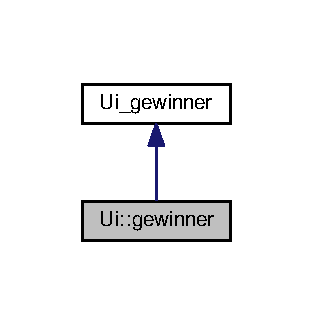
\includegraphics[width=150pt]{classUi_1_1gewinner__inherit__graph}
\end{center}
\end{figure}


Collaboration diagram for Ui\-:\-:gewinner\-:\nopagebreak
\begin{figure}[H]
\begin{center}
\leavevmode
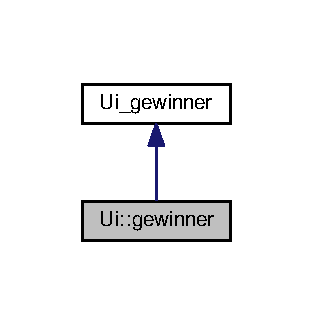
\includegraphics[width=150pt]{classUi_1_1gewinner__coll__graph}
\end{center}
\end{figure}
\subsection*{Additional Inherited Members}


The documentation for this class was generated from the following file\-:\begin{DoxyCompactItemize}
\item 
\hyperlink{ui__gewinner_8h}{ui\-\_\-gewinner.\-h}\end{DoxyCompactItemize}

\hypertarget{classgewinner}{\section{gewinner Class Reference}
\label{classgewinner}\index{gewinner@{gewinner}}
}


{\ttfamily \#include $<$gewinner.\-h$>$}



Inheritance diagram for gewinner\-:\nopagebreak
\begin{figure}[H]
\begin{center}
\leavevmode
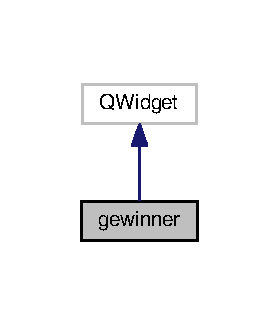
\includegraphics[width=134pt]{classgewinner__inherit__graph}
\end{center}
\end{figure}


Collaboration diagram for gewinner\-:\nopagebreak
\begin{figure}[H]
\begin{center}
\leavevmode
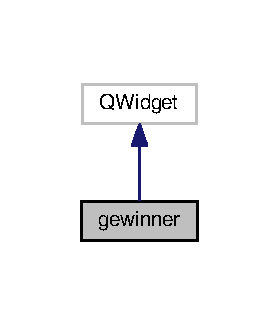
\includegraphics[width=134pt]{classgewinner__coll__graph}
\end{center}
\end{figure}
\subsection*{Public Member Functions}
\begin{DoxyCompactItemize}
\item 
\hyperlink{classgewinner_ae06130c27d9adbb780f33e0dc7ef1544}{gewinner} (Q\-Widget $\ast$parent=0, Q\-String \hyperlink{classgewinner}{gewinner}=\char`\"{}?\char`\"{})
\item 
\hyperlink{classgewinner_a99d0fdd7641b64d6e3fcf2d66f743185}{$\sim$gewinner} ()
\end{DoxyCompactItemize}


\subsection{Detailed Description}
Die Widget-\/\-Klasse gewinner, hat die Aufgabe zum Anzeigen eines Gewinners. 

\subsection{Constructor \& Destructor Documentation}
\hypertarget{classgewinner_ae06130c27d9adbb780f33e0dc7ef1544}{\index{gewinner@{gewinner}!gewinner@{gewinner}}
\index{gewinner@{gewinner}!gewinner@{gewinner}}
\subsubsection[{gewinner}]{\setlength{\rightskip}{0pt plus 5cm}gewinner\-::gewinner (
\begin{DoxyParamCaption}
\item[{Q\-Widget $\ast$}]{parent = {\ttfamily 0}, }
\item[{Q\-String}]{gewinner = {\ttfamily \char`\"{}?\char`\"{}}}
\end{DoxyParamCaption}
)\hspace{0.3cm}{\ttfamily [explicit]}}}\label{classgewinner_ae06130c27d9adbb780f33e0dc7ef1544}
Konstruiert das Gewinner-\/\-Widget, mit der Hilfe der Angabe des \char`\"{}\-Gewinner-\/\-Namens\char`\"{}.


\begin{DoxyParams}{Parameters}
{\em parent} & Die Angabe des Eltern-\/\-Widgets. \\
\hline
{\em gewinner} & Die Angabe des Namens des Gewinners. \\
\hline
\end{DoxyParams}


Here is the call graph for this function\-:\nopagebreak
\begin{figure}[H]
\begin{center}
\leavevmode
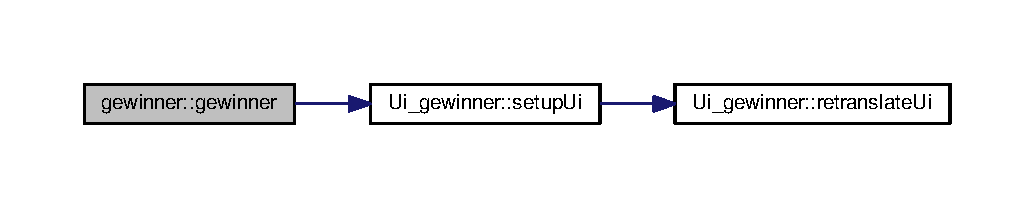
\includegraphics[width=350pt]{classgewinner_ae06130c27d9adbb780f33e0dc7ef1544_cgraph}
\end{center}
\end{figure}


\hypertarget{classgewinner_a99d0fdd7641b64d6e3fcf2d66f743185}{\index{gewinner@{gewinner}!$\sim$gewinner@{$\sim$gewinner}}
\index{$\sim$gewinner@{$\sim$gewinner}!gewinner@{gewinner}}
\subsubsection[{$\sim$gewinner}]{\setlength{\rightskip}{0pt plus 5cm}gewinner\-::$\sim$gewinner (
\begin{DoxyParamCaption}
{}
\end{DoxyParamCaption}
)}}\label{classgewinner_a99d0fdd7641b64d6e3fcf2d66f743185}
Destruktor des Gewinner-\/\-Widgets. 

The documentation for this class was generated from the following files\-:\begin{DoxyCompactItemize}
\item 
\hyperlink{gewinner_8h}{gewinner.\-h}\item 
\hyperlink{gewinner_8cpp}{gewinner.\-cpp}\end{DoxyCompactItemize}

\hypertarget{classGLWidget}{\section{G\-L\-Widget Class Reference}
\label{classGLWidget}\index{G\-L\-Widget@{G\-L\-Widget}}
}


{\ttfamily \#include $<$glwidget.\-h$>$}



Inheritance diagram for G\-L\-Widget\-:\nopagebreak
\begin{figure}[H]
\begin{center}
\leavevmode
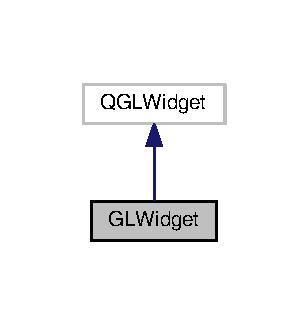
\includegraphics[width=148pt]{classGLWidget__inherit__graph}
\end{center}
\end{figure}


Collaboration diagram for G\-L\-Widget\-:\nopagebreak
\begin{figure}[H]
\begin{center}
\leavevmode
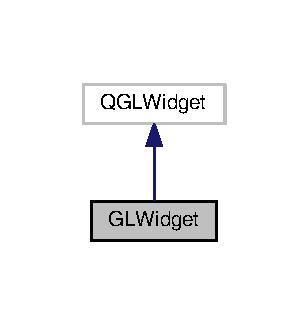
\includegraphics[width=148pt]{classGLWidget__coll__graph}
\end{center}
\end{figure}
\subsection*{Public Slots}
\begin{DoxyCompactItemize}
\item 
void \hyperlink{classGLWidget_a956079012f63513b1e9a5a764023553e}{update\-Game} ()
\item 
void \hyperlink{classGLWidget_a433268187ea9021a519991ff69a79a09}{setze\-Frage\-Spielzeug\-True} ()
\item 
void \hyperlink{classGLWidget_a236d12dd5c8593339b1bbe7c1350586b}{spiel\-Ende} (Q\-String gewinner\-Name)
\end{DoxyCompactItemize}
\subsection*{Signals}
\begin{DoxyCompactItemize}
\item 
void \hyperlink{classGLWidget_ab39fa82a1c9ebaf72705013d16b82ead}{spielfeld\-Clicked} (int, int)
\item 
void \hyperlink{classGLWidget_a364029cdf5543ec0a89ebc75033c94cf}{animation\-Done} ()
\end{DoxyCompactItemize}
\subsection*{Public Member Functions}
\begin{DoxyCompactItemize}
\item 
\hyperlink{classGLWidget_ab79c391c86de1ffb76f6950b49d82c0c}{G\-L\-Widget} (Q\-Widget $\ast$parent=0)
\item 
void \hyperlink{classGLWidget_a7fab13e8cc9fc0730ca54c08b2c923a7}{initialize\-G\-L} ()
\item 
void \hyperlink{classGLWidget_a640b5570cb2b37724fd5b58a77339c5e}{paint\-G\-L} ()
\item 
void \hyperlink{classGLWidget_a81d96c3a1f7b81ba1f8cd84e590d9bdc}{resize\-G\-L} (int breite, int hoehe)
\item 
void \hyperlink{classGLWidget_abe84c820e63e0471060ae8a52d22d48d}{zeichne\-Spielstein} (G\-L\-Uquadric\-Obj $\ast$quadrat)
\item 
void \hyperlink{classGLWidget_a6ce32f69bd43407acad1fcf6e24bad09}{zeichne\-Spielstein\-Layout} ()
\item 
void \hyperlink{classGLWidget_ab144cc8064c1bbf6d0ef0646ca0bd06c}{mouse\-Press\-Event} (Q\-Mouse\-Event $\ast$event)
\item 
Q\-Size \hyperlink{classGLWidget_afa31f139572999beb2e0d3de0c163059}{mindest\-Groesse} ()
\item 
Q\-Size \hyperlink{classGLWidget_ac19f12d5851509a8102251825c61e1c6}{spielfeld\-Groesse} ()
\item 
void \hyperlink{classGLWidget_a202b2be8dd40de28fd78f0d66a1a9b7d}{setze\-Frage\-Spielzug} (bool angabe\-Moeglich)
\item 
bool \hyperlink{classGLWidget_ad9250100246069a68437b5642ae5599f}{liefere\-Frage\-Spielzug} ()
\item 
bool \hyperlink{classGLWidget_a888efdb7d698d6603887846729eeee35}{liefere\-Animation} ()
\item 
bool \hyperlink{classGLWidget_a68054b4f43a10acf5718827a891df7e4}{liefere\-Animation\-Settings} ()
\item 
void \hyperlink{classGLWidget_a5fd50bbf7a81c7fafc320caff423f39b}{setze\-Animation} (bool angabe\-Bool)
\item 
void \hyperlink{classGLWidget_a7a0390510b6476b067b73d973be17adf}{setze\-Animation\-Settings} (bool angabe\-Bool)
\item 
void \hyperlink{classGLWidget_a868f792867edd549be3528fd498a03cf}{verbinde\-Spiel} (\hyperlink{classReversi}{Reversi} $\ast$spiel)
\item 
void \hyperlink{classGLWidget_a197a6b5236bea4840848ad36b9ebec67}{lege\-Spielerfest} (Q\-String spieler1\-Name, Q\-String spieler2\-Name, bool spieler1\-Black)
\end{DoxyCompactItemize}


\subsection{Detailed Description}
Die Klasse G\-L-\/\-Widget hat die Funktion zum anzeigen des Open\-G\-L-\/\-Kontents des Reversi-\/\-Spiels. 

\subsection{Constructor \& Destructor Documentation}
\hypertarget{classGLWidget_ab79c391c86de1ffb76f6950b49d82c0c}{\index{G\-L\-Widget@{G\-L\-Widget}!G\-L\-Widget@{G\-L\-Widget}}
\index{G\-L\-Widget@{G\-L\-Widget}!GLWidget@{G\-L\-Widget}}
\subsubsection[{G\-L\-Widget}]{\setlength{\rightskip}{0pt plus 5cm}G\-L\-Widget\-::\-G\-L\-Widget (
\begin{DoxyParamCaption}
\item[{Q\-Widget $\ast$}]{parent = {\ttfamily 0}}
\end{DoxyParamCaption}
)\hspace{0.3cm}{\ttfamily [explicit]}}}\label{classGLWidget_ab79c391c86de1ffb76f6950b49d82c0c}
Konstruiert ein G\-L-\/\-Widget, indem das komplette Reversispiel dargestellt wird.


\begin{DoxyParams}{Parameters}
{\em parent} & Die Angabe des Eltern-\/\-Widgets. \\
\hline
\end{DoxyParams}


Here is the call graph for this function\-:\nopagebreak
\begin{figure}[H]
\begin{center}
\leavevmode
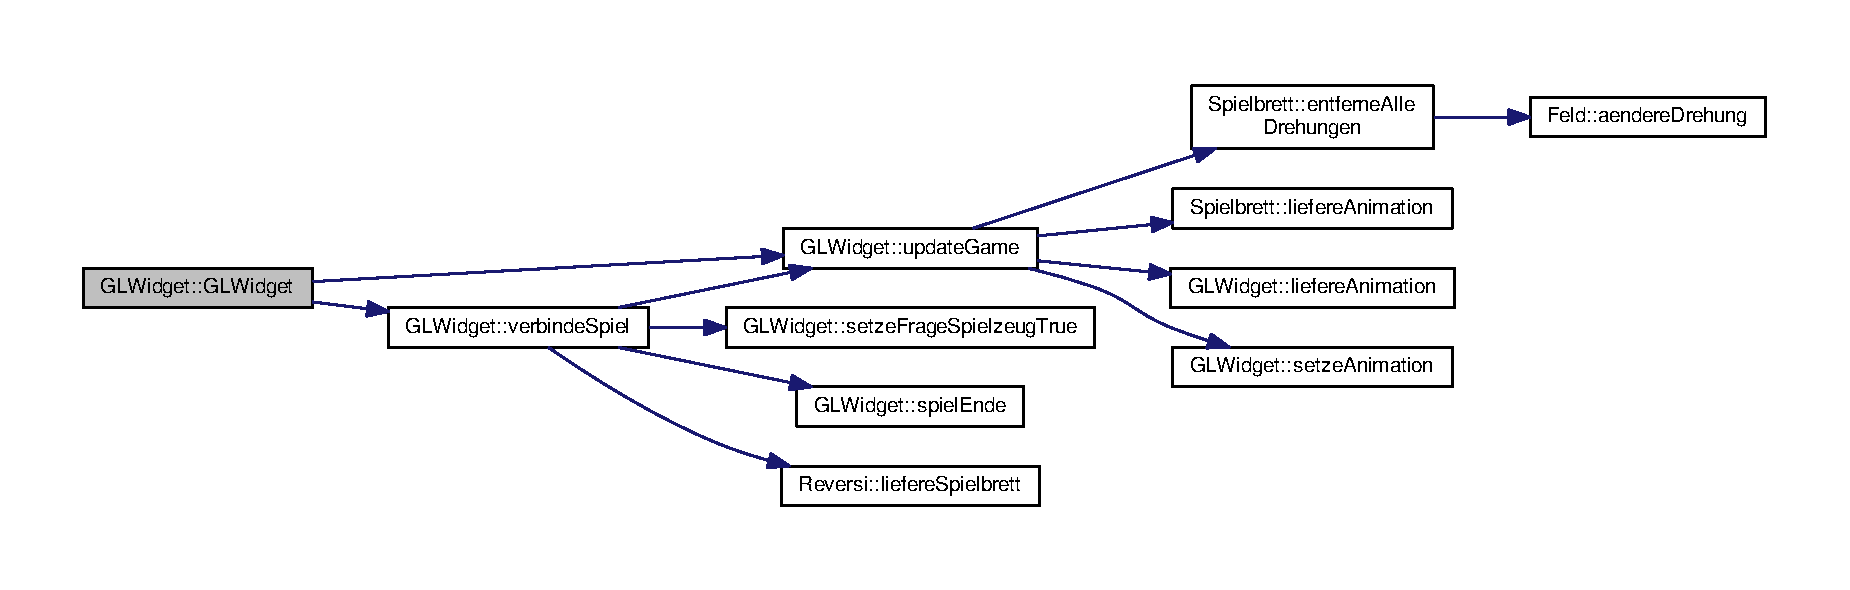
\includegraphics[width=350pt]{classGLWidget_ab79c391c86de1ffb76f6950b49d82c0c_cgraph}
\end{center}
\end{figure}




\subsection{Member Function Documentation}
\hypertarget{classGLWidget_a364029cdf5543ec0a89ebc75033c94cf}{\index{G\-L\-Widget@{G\-L\-Widget}!animation\-Done@{animation\-Done}}
\index{animation\-Done@{animation\-Done}!GLWidget@{G\-L\-Widget}}
\subsubsection[{animation\-Done}]{\setlength{\rightskip}{0pt plus 5cm}void G\-L\-Widget\-::animation\-Done (
\begin{DoxyParamCaption}
{}
\end{DoxyParamCaption}
)\hspace{0.3cm}{\ttfamily [signal]}}}\label{classGLWidget_a364029cdf5543ec0a89ebc75033c94cf}
Signal, dass alle Animationen beendet sind. \hypertarget{classGLWidget_a7fab13e8cc9fc0730ca54c08b2c923a7}{\index{G\-L\-Widget@{G\-L\-Widget}!initialize\-G\-L@{initialize\-G\-L}}
\index{initialize\-G\-L@{initialize\-G\-L}!GLWidget@{G\-L\-Widget}}
\subsubsection[{initialize\-G\-L}]{\setlength{\rightskip}{0pt plus 5cm}void G\-L\-Widget\-::initialize\-G\-L (
\begin{DoxyParamCaption}
{}
\end{DoxyParamCaption}
)}}\label{classGLWidget_a7fab13e8cc9fc0730ca54c08b2c923a7}
Initialisiert das G\-L-\/\-Widget, mit einer schwarzen Hintergrundfarbe und laed die Textur des Spielbretts. \hypertarget{classGLWidget_a197a6b5236bea4840848ad36b9ebec67}{\index{G\-L\-Widget@{G\-L\-Widget}!lege\-Spielerfest@{lege\-Spielerfest}}
\index{lege\-Spielerfest@{lege\-Spielerfest}!GLWidget@{G\-L\-Widget}}
\subsubsection[{lege\-Spielerfest}]{\setlength{\rightskip}{0pt plus 5cm}void G\-L\-Widget\-::lege\-Spielerfest (
\begin{DoxyParamCaption}
\item[{Q\-String}]{spieler1\-Name, }
\item[{Q\-String}]{spieler2\-Name, }
\item[{bool}]{spieler1\-Black}
\end{DoxyParamCaption}
)}}\label{classGLWidget_a197a6b5236bea4840848ad36b9ebec67}
Legt fest welcher \hyperlink{classSpieler}{Spieler} welchen Namen hat und welcher \hyperlink{classSpieler}{Spieler} welche farbe besitzt.


\begin{DoxyParams}{Parameters}
{\em spieler1\-Name} & Die Angabe des Namens von \hyperlink{classSpieler}{Spieler} 1. \\
\hline
{\em spieler2\-Name} & Die Angabe des Namens von \hyperlink{classSpieler}{Spieler} 2. \\
\hline
{\em spieler1\-Black} & Die Angabe welcher \hyperlink{classSpieler}{Spieler} der schwarze ist. (und damit beginnt) \\
\hline
\end{DoxyParams}


Here is the call graph for this function\-:\nopagebreak
\begin{figure}[H]
\begin{center}
\leavevmode
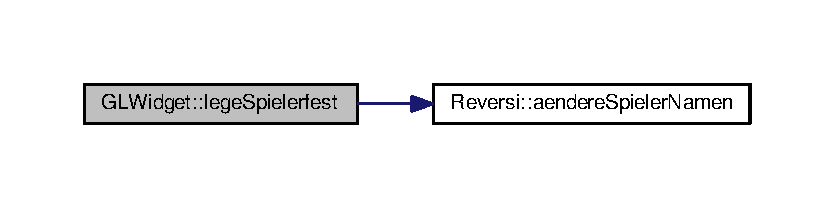
\includegraphics[width=350pt]{classGLWidget_a197a6b5236bea4840848ad36b9ebec67_cgraph}
\end{center}
\end{figure}


\hypertarget{classGLWidget_a888efdb7d698d6603887846729eeee35}{\index{G\-L\-Widget@{G\-L\-Widget}!liefere\-Animation@{liefere\-Animation}}
\index{liefere\-Animation@{liefere\-Animation}!GLWidget@{G\-L\-Widget}}
\subsubsection[{liefere\-Animation}]{\setlength{\rightskip}{0pt plus 5cm}bool G\-L\-Widget\-::liefere\-Animation (
\begin{DoxyParamCaption}
{}
\end{DoxyParamCaption}
)}}\label{classGLWidget_a888efdb7d698d6603887846729eeee35}
Liefert den boolschen Wert der Animation.

\begin{DoxyReturn}{Returns}
Den boolschen Wert der Animation. 
\end{DoxyReturn}
\hypertarget{classGLWidget_a68054b4f43a10acf5718827a891df7e4}{\index{G\-L\-Widget@{G\-L\-Widget}!liefere\-Animation\-Settings@{liefere\-Animation\-Settings}}
\index{liefere\-Animation\-Settings@{liefere\-Animation\-Settings}!GLWidget@{G\-L\-Widget}}
\subsubsection[{liefere\-Animation\-Settings}]{\setlength{\rightskip}{0pt plus 5cm}bool G\-L\-Widget\-::liefere\-Animation\-Settings (
\begin{DoxyParamCaption}
{}
\end{DoxyParamCaption}
)}}\label{classGLWidget_a68054b4f43a10acf5718827a891df7e4}
Liefert den boolschen Wert der Animation\-Settings.

\begin{DoxyReturn}{Returns}
Den boolschen Wert der Animation\-Settings. 
\end{DoxyReturn}
\hypertarget{classGLWidget_ad9250100246069a68437b5642ae5599f}{\index{G\-L\-Widget@{G\-L\-Widget}!liefere\-Frage\-Spielzug@{liefere\-Frage\-Spielzug}}
\index{liefere\-Frage\-Spielzug@{liefere\-Frage\-Spielzug}!GLWidget@{G\-L\-Widget}}
\subsubsection[{liefere\-Frage\-Spielzug}]{\setlength{\rightskip}{0pt plus 5cm}bool G\-L\-Widget\-::liefere\-Frage\-Spielzug (
\begin{DoxyParamCaption}
{}
\end{DoxyParamCaption}
)}}\label{classGLWidget_ad9250100246069a68437b5642ae5599f}
Liefert das frage\-Spielzug Attribut.

\begin{DoxyReturn}{Returns}
Das frage\-Spielzug Attribut. 
\end{DoxyReturn}
\hypertarget{classGLWidget_afa31f139572999beb2e0d3de0c163059}{\index{G\-L\-Widget@{G\-L\-Widget}!mindest\-Groesse@{mindest\-Groesse}}
\index{mindest\-Groesse@{mindest\-Groesse}!GLWidget@{G\-L\-Widget}}
\subsubsection[{mindest\-Groesse}]{\setlength{\rightskip}{0pt plus 5cm}Q\-Size G\-L\-Widget\-::mindest\-Groesse (
\begin{DoxyParamCaption}
{}
\end{DoxyParamCaption}
)}}\label{classGLWidget_afa31f139572999beb2e0d3de0c163059}
Liefert die Mindestgroesse des G\-L-\/\-Widgets, welche 600 $\ast$ 600 betraegt.

\begin{DoxyReturn}{Returns}
Die Mindestgroesse des G\-L-\/\-Widgets. 
\end{DoxyReturn}
\hypertarget{classGLWidget_ab144cc8064c1bbf6d0ef0646ca0bd06c}{\index{G\-L\-Widget@{G\-L\-Widget}!mouse\-Press\-Event@{mouse\-Press\-Event}}
\index{mouse\-Press\-Event@{mouse\-Press\-Event}!GLWidget@{G\-L\-Widget}}
\subsubsection[{mouse\-Press\-Event}]{\setlength{\rightskip}{0pt plus 5cm}void G\-L\-Widget\-::mouse\-Press\-Event (
\begin{DoxyParamCaption}
\item[{Q\-Mouse\-Event $\ast$}]{event}
\end{DoxyParamCaption}
)}}\label{classGLWidget_ab144cc8064c1bbf6d0ef0646ca0bd06c}
Event zum erfassen der Koordinaten eines Clicks. Wenn sich der Mausclick auf dem Spielfeld ereignet, wird das spiel\-Feld\-Clicked Signal ausgefuehrt.


\begin{DoxyParams}{Parameters}
{\em event} & Ein Q\-Mouse\-Event. \\
\hline
\end{DoxyParams}
\hypertarget{classGLWidget_a640b5570cb2b37724fd5b58a77339c5e}{\index{G\-L\-Widget@{G\-L\-Widget}!paint\-G\-L@{paint\-G\-L}}
\index{paint\-G\-L@{paint\-G\-L}!GLWidget@{G\-L\-Widget}}
\subsubsection[{paint\-G\-L}]{\setlength{\rightskip}{0pt plus 5cm}void G\-L\-Widget\-::paint\-G\-L (
\begin{DoxyParamCaption}
{}
\end{DoxyParamCaption}
)}}\label{classGLWidget_a640b5570cb2b37724fd5b58a77339c5e}
Zeichnet das aktuelle Bild in das G\-L-\/\-Widget. 

Here is the call graph for this function\-:\nopagebreak
\begin{figure}[H]
\begin{center}
\leavevmode
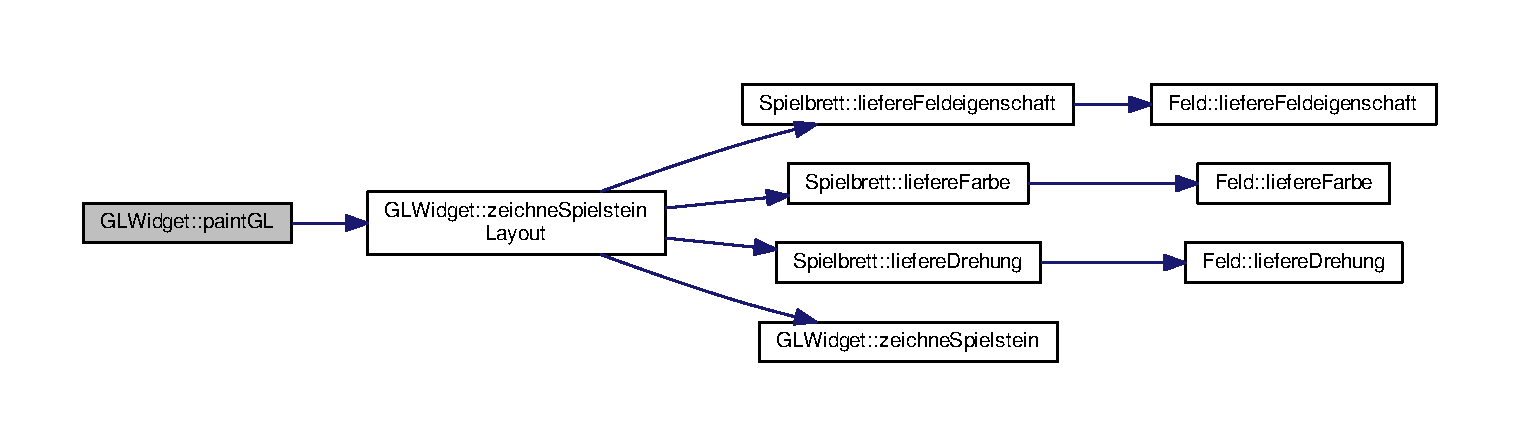
\includegraphics[width=350pt]{classGLWidget_a640b5570cb2b37724fd5b58a77339c5e_cgraph}
\end{center}
\end{figure}


\hypertarget{classGLWidget_a81d96c3a1f7b81ba1f8cd84e590d9bdc}{\index{G\-L\-Widget@{G\-L\-Widget}!resize\-G\-L@{resize\-G\-L}}
\index{resize\-G\-L@{resize\-G\-L}!GLWidget@{G\-L\-Widget}}
\subsubsection[{resize\-G\-L}]{\setlength{\rightskip}{0pt plus 5cm}void G\-L\-Widget\-::resize\-G\-L (
\begin{DoxyParamCaption}
\item[{int}]{breite, }
\item[{int}]{hoehe}
\end{DoxyParamCaption}
)}}\label{classGLWidget_a81d96c3a1f7b81ba1f8cd84e590d9bdc}
Standart-\/\-Methode eines G\-L\-Widgets zum Anpassen der groesse dessen in einem Fenster.


\begin{DoxyParams}{Parameters}
{\em breite} & Die Angabe der Breite des Fensters. \\
\hline
{\em hoehe} & Die Angabe der Hoehe des Fensters. \\
\hline
\end{DoxyParams}
\hypertarget{classGLWidget_a5fd50bbf7a81c7fafc320caff423f39b}{\index{G\-L\-Widget@{G\-L\-Widget}!setze\-Animation@{setze\-Animation}}
\index{setze\-Animation@{setze\-Animation}!GLWidget@{G\-L\-Widget}}
\subsubsection[{setze\-Animation}]{\setlength{\rightskip}{0pt plus 5cm}void G\-L\-Widget\-::setze\-Animation (
\begin{DoxyParamCaption}
\item[{bool}]{angabe\-Bool}
\end{DoxyParamCaption}
)}}\label{classGLWidget_a5fd50bbf7a81c7fafc320caff423f39b}
Setzt das animations Attribut.


\begin{DoxyParams}{Parameters}
{\em angabe\-Bool} & Angabe als boolscher Wert. \\
\hline
\end{DoxyParams}
\hypertarget{classGLWidget_a7a0390510b6476b067b73d973be17adf}{\index{G\-L\-Widget@{G\-L\-Widget}!setze\-Animation\-Settings@{setze\-Animation\-Settings}}
\index{setze\-Animation\-Settings@{setze\-Animation\-Settings}!GLWidget@{G\-L\-Widget}}
\subsubsection[{setze\-Animation\-Settings}]{\setlength{\rightskip}{0pt plus 5cm}void G\-L\-Widget\-::setze\-Animation\-Settings (
\begin{DoxyParamCaption}
\item[{bool}]{angabe\-Bool}
\end{DoxyParamCaption}
)}}\label{classGLWidget_a7a0390510b6476b067b73d973be17adf}
Setzt das animation\-Settings Attribut.


\begin{DoxyParams}{Parameters}
{\em angabe\-Bool} & Angabe als boolscher Wert. \\
\hline
\end{DoxyParams}
\hypertarget{classGLWidget_a433268187ea9021a519991ff69a79a09}{\index{G\-L\-Widget@{G\-L\-Widget}!setze\-Frage\-Spielzeug\-True@{setze\-Frage\-Spielzeug\-True}}
\index{setze\-Frage\-Spielzeug\-True@{setze\-Frage\-Spielzeug\-True}!GLWidget@{G\-L\-Widget}}
\subsubsection[{setze\-Frage\-Spielzeug\-True}]{\setlength{\rightskip}{0pt plus 5cm}void G\-L\-Widget\-::setze\-Frage\-Spielzeug\-True (
\begin{DoxyParamCaption}
{}
\end{DoxyParamCaption}
)\hspace{0.3cm}{\ttfamily [slot]}}}\label{classGLWidget_a433268187ea9021a519991ff69a79a09}
Setzt das frage\-Spielzug Attribut auf True. \hypertarget{classGLWidget_a202b2be8dd40de28fd78f0d66a1a9b7d}{\index{G\-L\-Widget@{G\-L\-Widget}!setze\-Frage\-Spielzug@{setze\-Frage\-Spielzug}}
\index{setze\-Frage\-Spielzug@{setze\-Frage\-Spielzug}!GLWidget@{G\-L\-Widget}}
\subsubsection[{setze\-Frage\-Spielzug}]{\setlength{\rightskip}{0pt plus 5cm}void G\-L\-Widget\-::setze\-Frage\-Spielzug (
\begin{DoxyParamCaption}
\item[{bool}]{angabe\-Moeglich}
\end{DoxyParamCaption}
)}}\label{classGLWidget_a202b2be8dd40de28fd78f0d66a1a9b7d}
Setzt das frage\-Spielzug Attribut.


\begin{DoxyParams}{Parameters}
{\em angabe\-Moeglich} & Angabe als boolscher Wert. \\
\hline
\end{DoxyParams}
\hypertarget{classGLWidget_a236d12dd5c8593339b1bbe7c1350586b}{\index{G\-L\-Widget@{G\-L\-Widget}!spiel\-Ende@{spiel\-Ende}}
\index{spiel\-Ende@{spiel\-Ende}!GLWidget@{G\-L\-Widget}}
\subsubsection[{spiel\-Ende}]{\setlength{\rightskip}{0pt plus 5cm}void G\-L\-Widget\-::spiel\-Ende (
\begin{DoxyParamCaption}
\item[{Q\-String}]{gewinner\-Name}
\end{DoxyParamCaption}
)\hspace{0.3cm}{\ttfamily [slot]}}}\label{classGLWidget_a236d12dd5c8593339b1bbe7c1350586b}
Zeigt das Gewinner-\/\-Widget an.


\begin{DoxyParams}{Parameters}
{\em gewinner\-Name} & Der Name des Gewinners. \\
\hline
\end{DoxyParams}
\hypertarget{classGLWidget_ab39fa82a1c9ebaf72705013d16b82ead}{\index{G\-L\-Widget@{G\-L\-Widget}!spielfeld\-Clicked@{spielfeld\-Clicked}}
\index{spielfeld\-Clicked@{spielfeld\-Clicked}!GLWidget@{G\-L\-Widget}}
\subsubsection[{spielfeld\-Clicked}]{\setlength{\rightskip}{0pt plus 5cm}void G\-L\-Widget\-::spielfeld\-Clicked (
\begin{DoxyParamCaption}
\item[{int}]{, }
\item[{int}]{}
\end{DoxyParamCaption}
)\hspace{0.3cm}{\ttfamily [signal]}}}\label{classGLWidget_ab39fa82a1c9ebaf72705013d16b82ead}
Signal, dass das Spielfeld geclickt wurde. \hypertarget{classGLWidget_ac19f12d5851509a8102251825c61e1c6}{\index{G\-L\-Widget@{G\-L\-Widget}!spielfeld\-Groesse@{spielfeld\-Groesse}}
\index{spielfeld\-Groesse@{spielfeld\-Groesse}!GLWidget@{G\-L\-Widget}}
\subsubsection[{spielfeld\-Groesse}]{\setlength{\rightskip}{0pt plus 5cm}Q\-Size G\-L\-Widget\-::spielfeld\-Groesse (
\begin{DoxyParamCaption}
{}
\end{DoxyParamCaption}
)}}\label{classGLWidget_ac19f12d5851509a8102251825c61e1c6}
Liefert die Mindestgroesse des Spielfeldes, welches 500 $\ast$ 500 betraegt.

\begin{DoxyReturn}{Returns}
Die Mindestgroesse des Spielfeldes. 
\end{DoxyReturn}
\hypertarget{classGLWidget_a956079012f63513b1e9a5a764023553e}{\index{G\-L\-Widget@{G\-L\-Widget}!update\-Game@{update\-Game}}
\index{update\-Game@{update\-Game}!GLWidget@{G\-L\-Widget}}
\subsubsection[{update\-Game}]{\setlength{\rightskip}{0pt plus 5cm}void G\-L\-Widget\-::update\-Game (
\begin{DoxyParamCaption}
{}
\end{DoxyParamCaption}
)\hspace{0.3cm}{\ttfamily [slot]}}}\label{classGLWidget_a956079012f63513b1e9a5a764023553e}
Fuehrt alle Aenderungen an den Spielsteinen aus, und dreht diese um 180 Grad, wenn sich deren Farbe aendert. 

Here is the call graph for this function\-:\nopagebreak
\begin{figure}[H]
\begin{center}
\leavevmode
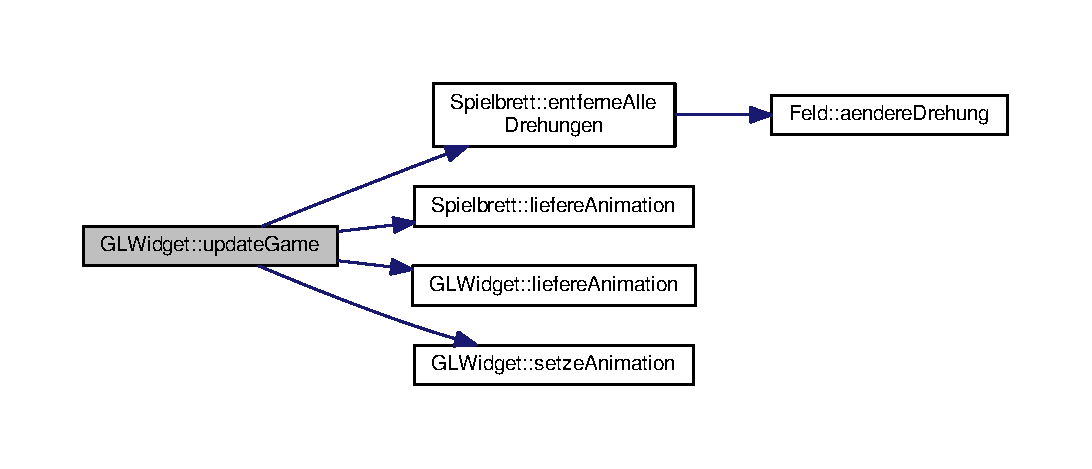
\includegraphics[width=350pt]{classGLWidget_a956079012f63513b1e9a5a764023553e_cgraph}
\end{center}
\end{figure}


\hypertarget{classGLWidget_a868f792867edd549be3528fd498a03cf}{\index{G\-L\-Widget@{G\-L\-Widget}!verbinde\-Spiel@{verbinde\-Spiel}}
\index{verbinde\-Spiel@{verbinde\-Spiel}!GLWidget@{G\-L\-Widget}}
\subsubsection[{verbinde\-Spiel}]{\setlength{\rightskip}{0pt plus 5cm}void G\-L\-Widget\-::verbinde\-Spiel (
\begin{DoxyParamCaption}
\item[{{\bf Reversi} $\ast$}]{spiel}
\end{DoxyParamCaption}
)}}\label{classGLWidget_a868f792867edd549be3528fd498a03cf}
Verbindet das G\-L-\/\-Widget mit einem Reversi-\/\-Objekt. Ueber Signals und Slots werden ereignisse ausgetauscht, wie z.\-B. das setzen eines Spielsteins oder wechsel des aktuellen Spielers etc..

(Verbindet G\-L-\/\-Widget mit der Reversi-\/\-Logik)


\begin{DoxyParams}{Parameters}
{\em spiel} & Die Angabe des Reversi-\/\-Spiel Objekts. \\
\hline
\end{DoxyParams}


Here is the call graph for this function\-:\nopagebreak
\begin{figure}[H]
\begin{center}
\leavevmode
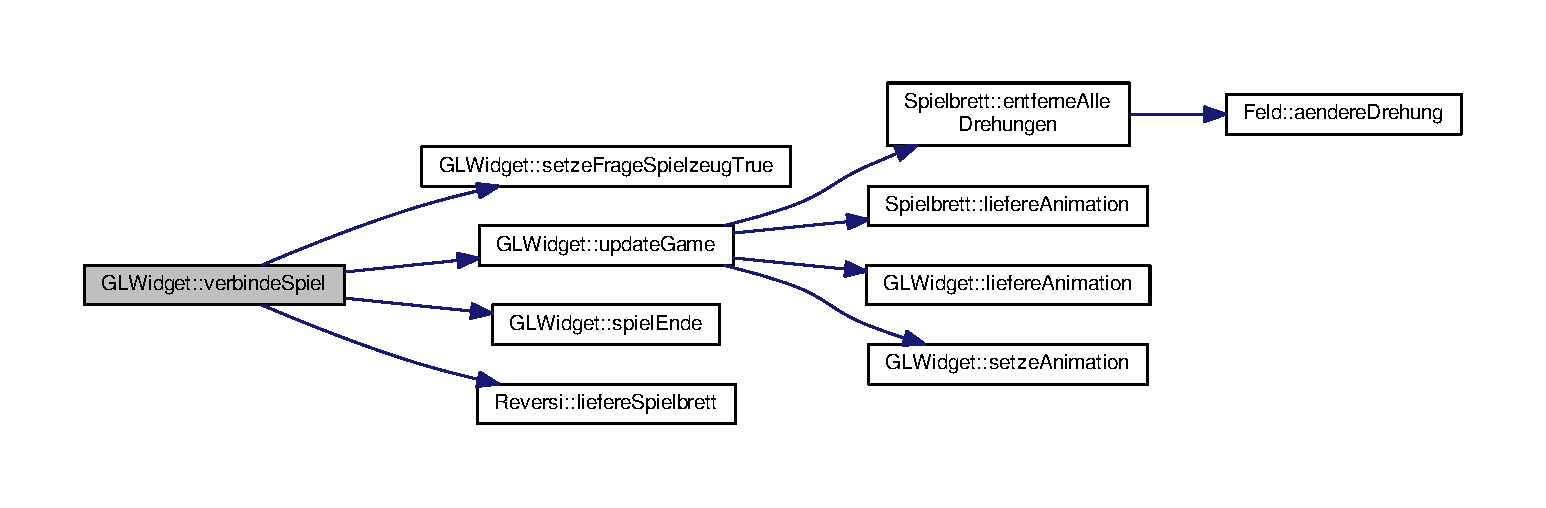
\includegraphics[width=350pt]{classGLWidget_a868f792867edd549be3528fd498a03cf_cgraph}
\end{center}
\end{figure}


\hypertarget{classGLWidget_abe84c820e63e0471060ae8a52d22d48d}{\index{G\-L\-Widget@{G\-L\-Widget}!zeichne\-Spielstein@{zeichne\-Spielstein}}
\index{zeichne\-Spielstein@{zeichne\-Spielstein}!GLWidget@{G\-L\-Widget}}
\subsubsection[{zeichne\-Spielstein}]{\setlength{\rightskip}{0pt plus 5cm}void G\-L\-Widget\-::zeichne\-Spielstein (
\begin{DoxyParamCaption}
\item[{G\-L\-Uquadric\-Obj $\ast$}]{quadrat}
\end{DoxyParamCaption}
)}}\label{classGLWidget_abe84c820e63e0471060ae8a52d22d48d}
Veraendert ein Quadrat zu einem ovalfoermigen Spielstein mit einer schwarzen und weissen seite und Zeichnet diesen in das G\-L-\/\-Widget.


\begin{DoxyParams}{Parameters}
{\em quadrat} & Angbae eines G\-L\-Quadrats, welches zu einem Spielstein transformiert werden soll. \\
\hline
\end{DoxyParams}
\hypertarget{classGLWidget_a6ce32f69bd43407acad1fcf6e24bad09}{\index{G\-L\-Widget@{G\-L\-Widget}!zeichne\-Spielstein\-Layout@{zeichne\-Spielstein\-Layout}}
\index{zeichne\-Spielstein\-Layout@{zeichne\-Spielstein\-Layout}!GLWidget@{G\-L\-Widget}}
\subsubsection[{zeichne\-Spielstein\-Layout}]{\setlength{\rightskip}{0pt plus 5cm}void G\-L\-Widget\-::zeichne\-Spielstein\-Layout (
\begin{DoxyParamCaption}
{}
\end{DoxyParamCaption}
)}}\label{classGLWidget_a6ce32f69bd43407acad1fcf6e24bad09}
Zeichent die Spielsteine auf das \hyperlink{classSpielbrett}{Spielbrett} und fuehrt die Drehungen dieser durch, wenn sich deren Farbe aendert. 

Here is the call graph for this function\-:\nopagebreak
\begin{figure}[H]
\begin{center}
\leavevmode
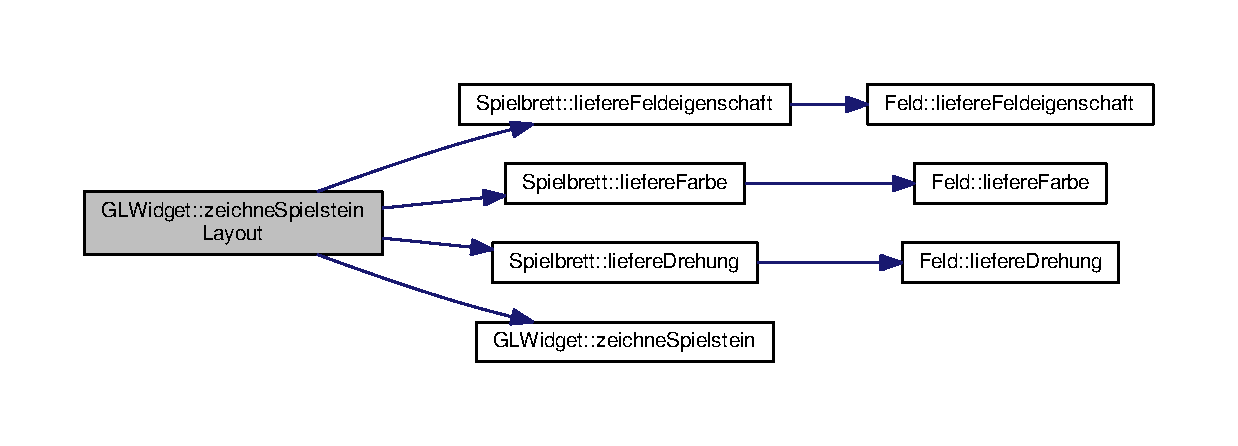
\includegraphics[width=350pt]{classGLWidget_a6ce32f69bd43407acad1fcf6e24bad09_cgraph}
\end{center}
\end{figure}




The documentation for this class was generated from the following files\-:\begin{DoxyCompactItemize}
\item 
\hyperlink{glwidget_8h}{glwidget.\-h}\item 
\hyperlink{glwidget_8cpp}{glwidget.\-cpp}\end{DoxyCompactItemize}

\hypertarget{classHauptmenue}{\section{Hauptmenue Class Reference}
\label{classHauptmenue}\index{Hauptmenue@{Hauptmenue}}
}


{\ttfamily \#include $<$hauptmenue.\-h$>$}



Inheritance diagram for Hauptmenue\-:\nopagebreak
\begin{figure}[H]
\begin{center}
\leavevmode
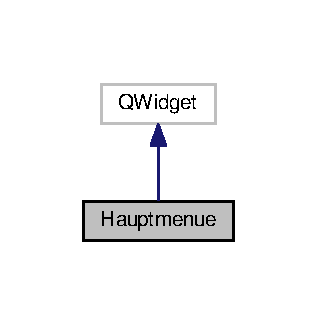
\includegraphics[width=152pt]{classHauptmenue__inherit__graph}
\end{center}
\end{figure}


Collaboration diagram for Hauptmenue\-:\nopagebreak
\begin{figure}[H]
\begin{center}
\leavevmode
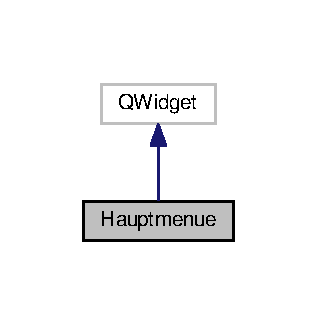
\includegraphics[width=152pt]{classHauptmenue__coll__graph}
\end{center}
\end{figure}
\subsection*{Public Member Functions}
\begin{DoxyCompactItemize}
\item 
\hyperlink{classHauptmenue_a3ece44e72084e49c9d0f2fa22deff21a}{Hauptmenue} (Q\-Widget $\ast$parent=0, Q\-Stacked\-Widget $\ast$the\-Sites=0)
\item 
\hyperlink{classHauptmenue_a5cccffcca3ecce4dfa41fe6fe9d7cb0d}{$\sim$\-Hauptmenue} ()
\end{DoxyCompactItemize}


\subsection{Detailed Description}
Die Hauptmenue-\/\-Widget Klasse bietet die Funktionen zum Navigieren durch das Programm. 

\subsection{Constructor \& Destructor Documentation}
\hypertarget{classHauptmenue_a3ece44e72084e49c9d0f2fa22deff21a}{\index{Hauptmenue@{Hauptmenue}!Hauptmenue@{Hauptmenue}}
\index{Hauptmenue@{Hauptmenue}!Hauptmenue@{Hauptmenue}}
\subsubsection[{Hauptmenue}]{\setlength{\rightskip}{0pt plus 5cm}Hauptmenue\-::\-Hauptmenue (
\begin{DoxyParamCaption}
\item[{Q\-Widget $\ast$}]{parent = {\ttfamily 0}, }
\item[{Q\-Stacked\-Widget $\ast$}]{the\-Sites = {\ttfamily 0}}
\end{DoxyParamCaption}
)\hspace{0.3cm}{\ttfamily [explicit]}}}\label{classHauptmenue_a3ece44e72084e49c9d0f2fa22deff21a}
Konstruktor fuer das Hauptmenue-\/\-Widget.


\begin{DoxyParams}{Parameters}
{\em parent} & Das Elternwidget. \\
\hline
{\em the\-Sites} & Die Angabe der zu navigierbaren Widgets. \\
\hline
\end{DoxyParams}


Here is the call graph for this function\-:\nopagebreak
\begin{figure}[H]
\begin{center}
\leavevmode
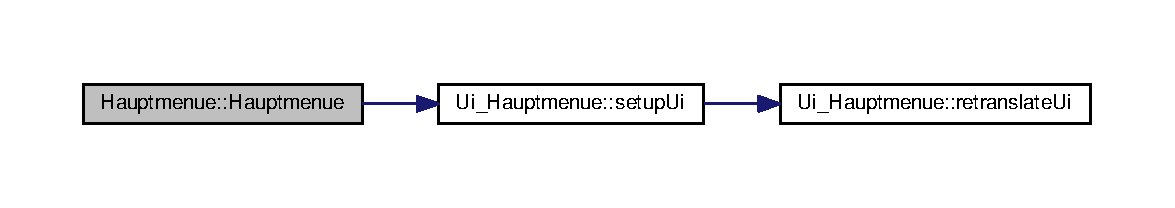
\includegraphics[width=350pt]{classHauptmenue_a3ece44e72084e49c9d0f2fa22deff21a_cgraph}
\end{center}
\end{figure}


\hypertarget{classHauptmenue_a5cccffcca3ecce4dfa41fe6fe9d7cb0d}{\index{Hauptmenue@{Hauptmenue}!$\sim$\-Hauptmenue@{$\sim$\-Hauptmenue}}
\index{$\sim$\-Hauptmenue@{$\sim$\-Hauptmenue}!Hauptmenue@{Hauptmenue}}
\subsubsection[{$\sim$\-Hauptmenue}]{\setlength{\rightskip}{0pt plus 5cm}Hauptmenue\-::$\sim$\-Hauptmenue (
\begin{DoxyParamCaption}
{}
\end{DoxyParamCaption}
)}}\label{classHauptmenue_a5cccffcca3ecce4dfa41fe6fe9d7cb0d}
Destructor fuer das Hauptmenue-\/\-Widget. 

The documentation for this class was generated from the following files\-:\begin{DoxyCompactItemize}
\item 
\hyperlink{hauptmenue_8h}{hauptmenue.\-h}\item 
\hyperlink{hauptmenue_8cpp}{hauptmenue.\-cpp}\end{DoxyCompactItemize}

\hypertarget{classUi_1_1Hauptmenue}{\section{Ui\-:\-:Hauptmenue Class Reference}
\label{classUi_1_1Hauptmenue}\index{Ui\-::\-Hauptmenue@{Ui\-::\-Hauptmenue}}
}


{\ttfamily \#include $<$ui\-\_\-hauptmenue.\-h$>$}



Inheritance diagram for Ui\-:\-:Hauptmenue\-:\nopagebreak
\begin{figure}[H]
\begin{center}
\leavevmode
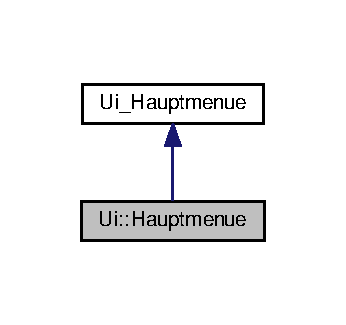
\includegraphics[width=166pt]{classUi_1_1Hauptmenue__inherit__graph}
\end{center}
\end{figure}


Collaboration diagram for Ui\-:\-:Hauptmenue\-:\nopagebreak
\begin{figure}[H]
\begin{center}
\leavevmode
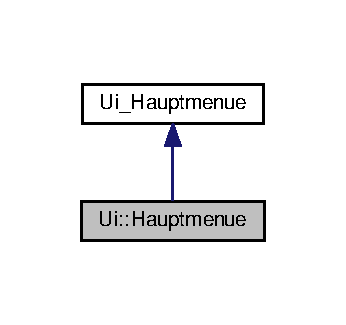
\includegraphics[width=166pt]{classUi_1_1Hauptmenue__coll__graph}
\end{center}
\end{figure}
\subsection*{Additional Inherited Members}


The documentation for this class was generated from the following file\-:\begin{DoxyCompactItemize}
\item 
\hyperlink{ui__hauptmenue_8h}{ui\-\_\-hauptmenue.\-h}\end{DoxyCompactItemize}

\hypertarget{classUi_1_1MainWindow}{\section{Ui\-:\-:Main\-Window Class Reference}
\label{classUi_1_1MainWindow}\index{Ui\-::\-Main\-Window@{Ui\-::\-Main\-Window}}
}


{\ttfamily \#include $<$ui\-\_\-mainwindow.\-h$>$}



Inheritance diagram for Ui\-:\-:Main\-Window\-:\nopagebreak
\begin{figure}[H]
\begin{center}
\leavevmode
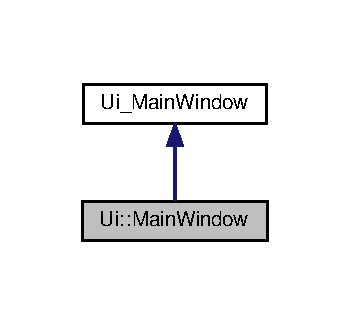
\includegraphics[width=168pt]{classUi_1_1MainWindow__inherit__graph}
\end{center}
\end{figure}


Collaboration diagram for Ui\-:\-:Main\-Window\-:\nopagebreak
\begin{figure}[H]
\begin{center}
\leavevmode
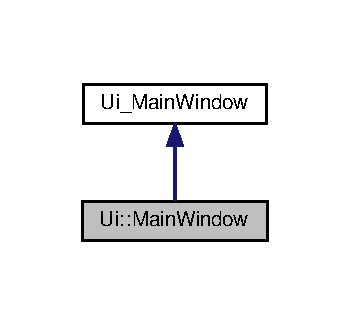
\includegraphics[width=168pt]{classUi_1_1MainWindow__coll__graph}
\end{center}
\end{figure}
\subsection*{Additional Inherited Members}


The documentation for this class was generated from the following file\-:\begin{DoxyCompactItemize}
\item 
\hyperlink{ui__mainwindow_8h}{ui\-\_\-mainwindow.\-h}\end{DoxyCompactItemize}

\hypertarget{classMainWindow}{\section{Main\-Window Class Reference}
\label{classMainWindow}\index{Main\-Window@{Main\-Window}}
}


{\ttfamily \#include $<$mainwindow.\-h$>$}



Inheritance diagram for Main\-Window\-:\nopagebreak
\begin{figure}[H]
\begin{center}
\leavevmode
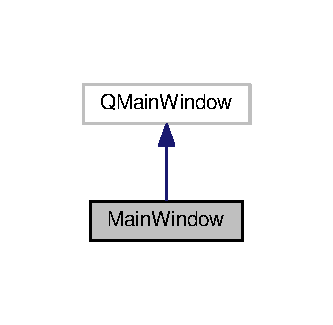
\includegraphics[width=160pt]{classMainWindow__inherit__graph}
\end{center}
\end{figure}


Collaboration diagram for Main\-Window\-:\nopagebreak
\begin{figure}[H]
\begin{center}
\leavevmode
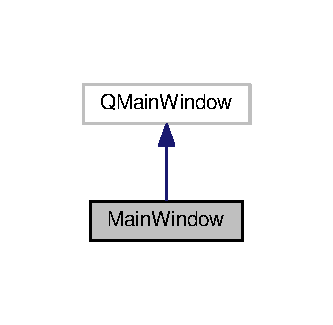
\includegraphics[width=160pt]{classMainWindow__coll__graph}
\end{center}
\end{figure}
\subsection*{Public Member Functions}
\begin{DoxyCompactItemize}
\item 
\hyperlink{classMainWindow_a8b244be8b7b7db1b08de2a2acb9409db}{Main\-Window} (Q\-Widget $\ast$parent=0)
\item 
\hyperlink{classMainWindow_ae98d00a93bc118200eeef9f9bba1dba7}{$\sim$\-Main\-Window} ()
\end{DoxyCompactItemize}


\subsection{Detailed Description}
Die Main-\/\-Windows Klasse stellt das Hauptfenster bereit, indem die Applikation dargestellt wird. 

\subsection{Constructor \& Destructor Documentation}
\hypertarget{classMainWindow_a8b244be8b7b7db1b08de2a2acb9409db}{\index{Main\-Window@{Main\-Window}!Main\-Window@{Main\-Window}}
\index{Main\-Window@{Main\-Window}!MainWindow@{Main\-Window}}
\subsubsection[{Main\-Window}]{\setlength{\rightskip}{0pt plus 5cm}Main\-Window\-::\-Main\-Window (
\begin{DoxyParamCaption}
\item[{Q\-Widget $\ast$}]{parent = {\ttfamily 0}}
\end{DoxyParamCaption}
)\hspace{0.3cm}{\ttfamily [explicit]}}}\label{classMainWindow_a8b244be8b7b7db1b08de2a2acb9409db}
Konstruktor fuer ein Main\-Window-\/\-Objekt. In diesem Objekt werden alle weiteren Widgets geladen. 

Here is the call graph for this function\-:\nopagebreak
\begin{figure}[H]
\begin{center}
\leavevmode
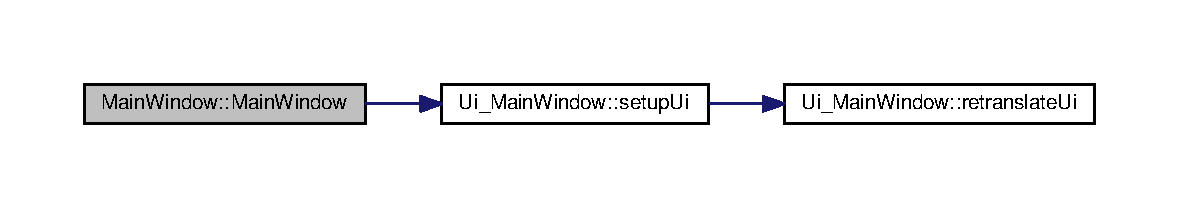
\includegraphics[width=350pt]{classMainWindow_a8b244be8b7b7db1b08de2a2acb9409db_cgraph}
\end{center}
\end{figure}


\hypertarget{classMainWindow_ae98d00a93bc118200eeef9f9bba1dba7}{\index{Main\-Window@{Main\-Window}!$\sim$\-Main\-Window@{$\sim$\-Main\-Window}}
\index{$\sim$\-Main\-Window@{$\sim$\-Main\-Window}!MainWindow@{Main\-Window}}
\subsubsection[{$\sim$\-Main\-Window}]{\setlength{\rightskip}{0pt plus 5cm}Main\-Window\-::$\sim$\-Main\-Window (
\begin{DoxyParamCaption}
{}
\end{DoxyParamCaption}
)}}\label{classMainWindow_ae98d00a93bc118200eeef9f9bba1dba7}
Destructor der \hyperlink{classMainWindow}{Main\-Window} Klasse. 

The documentation for this class was generated from the following files\-:\begin{DoxyCompactItemize}
\item 
\hyperlink{mainwindow_8h}{mainwindow.\-h}\item 
\hyperlink{mainwindow_8cpp}{mainwindow.\-cpp}\end{DoxyCompactItemize}

\hypertarget{classUi_1_1newGame}{\section{Ui\-:\-:new\-Game Class Reference}
\label{classUi_1_1newGame}\index{Ui\-::new\-Game@{Ui\-::new\-Game}}
}


{\ttfamily \#include $<$ui\-\_\-newgame.\-h$>$}



Inheritance diagram for Ui\-:\-:new\-Game\-:\nopagebreak
\begin{figure}[H]
\begin{center}
\leavevmode
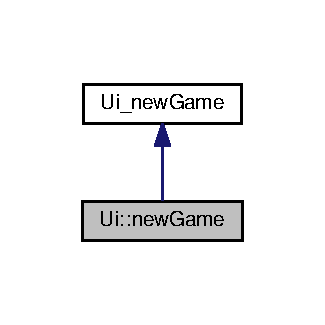
\includegraphics[width=156pt]{classUi_1_1newGame__inherit__graph}
\end{center}
\end{figure}


Collaboration diagram for Ui\-:\-:new\-Game\-:\nopagebreak
\begin{figure}[H]
\begin{center}
\leavevmode
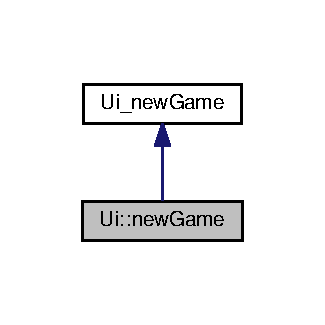
\includegraphics[width=156pt]{classUi_1_1newGame__coll__graph}
\end{center}
\end{figure}
\subsection*{Additional Inherited Members}


The documentation for this class was generated from the following file\-:\begin{DoxyCompactItemize}
\item 
\hyperlink{ui__newgame_8h}{ui\-\_\-newgame.\-h}\end{DoxyCompactItemize}

\hypertarget{classnewGame}{\section{new\-Game Class Reference}
\label{classnewGame}\index{new\-Game@{new\-Game}}
}


{\ttfamily \#include $<$newgame.\-h$>$}



Inheritance diagram for new\-Game\-:\nopagebreak
\begin{figure}[H]
\begin{center}
\leavevmode
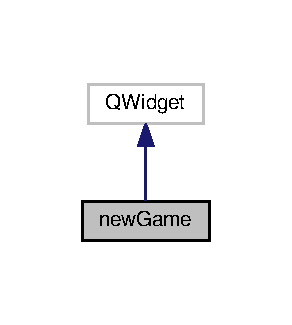
\includegraphics[width=140pt]{classnewGame__inherit__graph}
\end{center}
\end{figure}


Collaboration diagram for new\-Game\-:\nopagebreak
\begin{figure}[H]
\begin{center}
\leavevmode
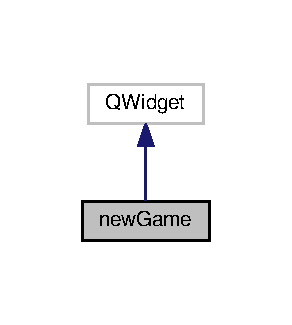
\includegraphics[width=140pt]{classnewGame__coll__graph}
\end{center}
\end{figure}
\subsection*{Public Member Functions}
\begin{DoxyCompactItemize}
\item 
\hyperlink{classnewGame_ae1e2ce2bd0fa9e708ad26492a60d61e0}{new\-Game} (Q\-Widget $\ast$parent=0, Q\-Stacked\-Widget $\ast$the\-Sites=0)
\item 
\hyperlink{classnewGame_a90b523a2249c54255d529c4cb3473e94}{$\sim$new\-Game} ()
\end{DoxyCompactItemize}


\subsection{Detailed Description}
Die New\-Game-\/\-Klasse ist ein Widget, welches das User\-Interface zum erstellen eines neuen Reversispiels bereitstellt. 

\subsection{Constructor \& Destructor Documentation}
\hypertarget{classnewGame_ae1e2ce2bd0fa9e708ad26492a60d61e0}{\index{new\-Game@{new\-Game}!new\-Game@{new\-Game}}
\index{new\-Game@{new\-Game}!newGame@{new\-Game}}
\subsubsection[{new\-Game}]{\setlength{\rightskip}{0pt plus 5cm}new\-Game\-::new\-Game (
\begin{DoxyParamCaption}
\item[{Q\-Widget $\ast$}]{parent = {\ttfamily 0}, }
\item[{Q\-Stacked\-Widget $\ast$}]{the\-Sites = {\ttfamily 0}}
\end{DoxyParamCaption}
)\hspace{0.3cm}{\ttfamily [explicit]}}}\label{classnewGame_ae1e2ce2bd0fa9e708ad26492a60d61e0}
Konstruktor fuer ein new\-Game-\/\-Widget.


\begin{DoxyParams}{Parameters}
{\em parent} & Die Angabe des Parentwidgets. \\
\hline
{\em the\-Sites} & Die Angabe der zu erreichenden Widgets. \\
\hline
\end{DoxyParams}


Here is the call graph for this function\-:\nopagebreak
\begin{figure}[H]
\begin{center}
\leavevmode
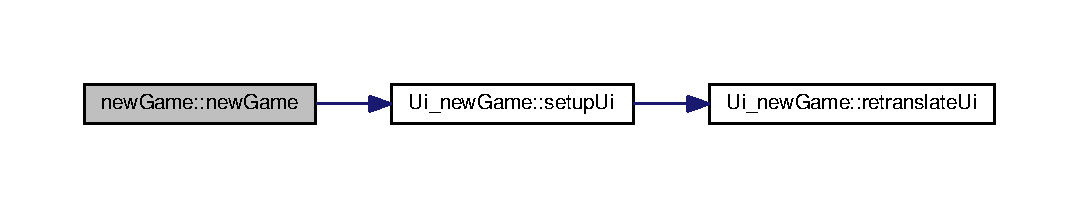
\includegraphics[width=350pt]{classnewGame_ae1e2ce2bd0fa9e708ad26492a60d61e0_cgraph}
\end{center}
\end{figure}


\hypertarget{classnewGame_a90b523a2249c54255d529c4cb3473e94}{\index{new\-Game@{new\-Game}!$\sim$new\-Game@{$\sim$new\-Game}}
\index{$\sim$new\-Game@{$\sim$new\-Game}!newGame@{new\-Game}}
\subsubsection[{$\sim$new\-Game}]{\setlength{\rightskip}{0pt plus 5cm}new\-Game\-::$\sim$new\-Game (
\begin{DoxyParamCaption}
{}
\end{DoxyParamCaption}
)}}\label{classnewGame_a90b523a2249c54255d529c4cb3473e94}
Destruktor der \hyperlink{classnewGame}{new\-Game} Klasse. 

The documentation for this class was generated from the following files\-:\begin{DoxyCompactItemize}
\item 
\hyperlink{newgame_8h}{newgame.\-h}\item 
\hyperlink{newgame_8cpp}{newgame.\-cpp}\end{DoxyCompactItemize}

\hypertarget{classOpenGLGame}{\section{Open\-G\-L\-Game Class Reference}
\label{classOpenGLGame}\index{Open\-G\-L\-Game@{Open\-G\-L\-Game}}
}


{\ttfamily \#include $<$openglgame.\-h$>$}



Inheritance diagram for Open\-G\-L\-Game\-:\nopagebreak
\begin{figure}[H]
\begin{center}
\leavevmode
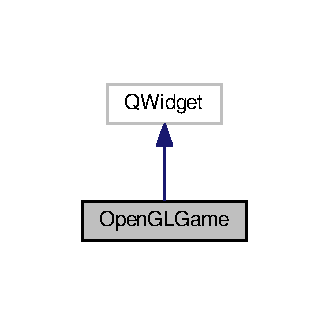
\includegraphics[width=158pt]{classOpenGLGame__inherit__graph}
\end{center}
\end{figure}


Collaboration diagram for Open\-G\-L\-Game\-:\nopagebreak
\begin{figure}[H]
\begin{center}
\leavevmode
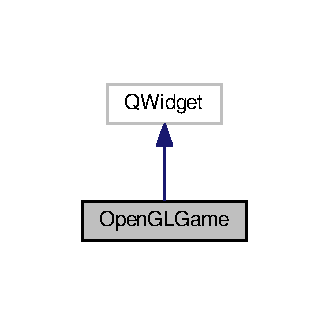
\includegraphics[width=158pt]{classOpenGLGame__coll__graph}
\end{center}
\end{figure}
\subsection*{Public Member Functions}
\begin{DoxyCompactItemize}
\item 
\hyperlink{classOpenGLGame_a9082f6e7cad74cd49dab386bf14dc185}{Open\-G\-L\-Game} (Q\-Widget $\ast$parent=0, Q\-Stacked\-Widget $\ast$the\-Sites=0, Q\-String spielername1=\char`\"{}Spieler 1\char`\"{}, Q\-String spielername2=\char`\"{}Spieler 2\char`\"{}, bool spieler1black=true)
\item 
\hyperlink{classOpenGLGame_a20705f1f3f495f65f2879681a20eb43b}{$\sim$\-Open\-G\-L\-Game} ()
\end{DoxyCompactItemize}


\subsection{Detailed Description}
Die \hyperlink{classOpenGLGame}{Open\-G\-L\-Game} Widget Klasse, stellt das Fenster fuer ein Reversi-\/\-G\-L\-Widget bereit. 

\subsection{Constructor \& Destructor Documentation}
\hypertarget{classOpenGLGame_a9082f6e7cad74cd49dab386bf14dc185}{\index{Open\-G\-L\-Game@{Open\-G\-L\-Game}!Open\-G\-L\-Game@{Open\-G\-L\-Game}}
\index{Open\-G\-L\-Game@{Open\-G\-L\-Game}!OpenGLGame@{Open\-G\-L\-Game}}
\subsubsection[{Open\-G\-L\-Game}]{\setlength{\rightskip}{0pt plus 5cm}Open\-G\-L\-Game\-::\-Open\-G\-L\-Game (
\begin{DoxyParamCaption}
\item[{Q\-Widget $\ast$}]{parent = {\ttfamily 0}, }
\item[{Q\-Stacked\-Widget $\ast$}]{the\-Sites = {\ttfamily 0}, }
\item[{Q\-String}]{spielername1 = {\ttfamily \char`\"{}Spieler~1\char`\"{}}, }
\item[{Q\-String}]{spielername2 = {\ttfamily \char`\"{}Spieler~2\char`\"{}}, }
\item[{bool}]{spieler1black = {\ttfamily true}}
\end{DoxyParamCaption}
)\hspace{0.3cm}{\ttfamily [explicit]}}}\label{classOpenGLGame_a9082f6e7cad74cd49dab386bf14dc185}
Konstruktor fuer ein Open\-Gl\-Game-\/\-Widget. Gibt die Spielernamen und welcher \hyperlink{classSpieler}{Spieler} startet an das \hyperlink{classGLWidget}{G\-L\-Widget} weiter.


\begin{DoxyParams}{Parameters}
{\em parent} & Die Angabe vom Eltern\-Widget. \\
\hline
{\em the\-Sites} & Alle Widgets, zu welchen navigiert werden kann. \\
\hline
{\em spielername1} & Die Angabe des Spielernamens. \\
\hline
{\em spielername2} & Die Angabe des Spielernamens. \\
\hline
{\em spieler1black} & Die Angabe welcher \hyperlink{classSpieler}{Spieler} die schwarzen Spielsteine besitzt. \\
\hline
\end{DoxyParams}


Here is the call graph for this function\-:\nopagebreak
\begin{figure}[H]
\begin{center}
\leavevmode
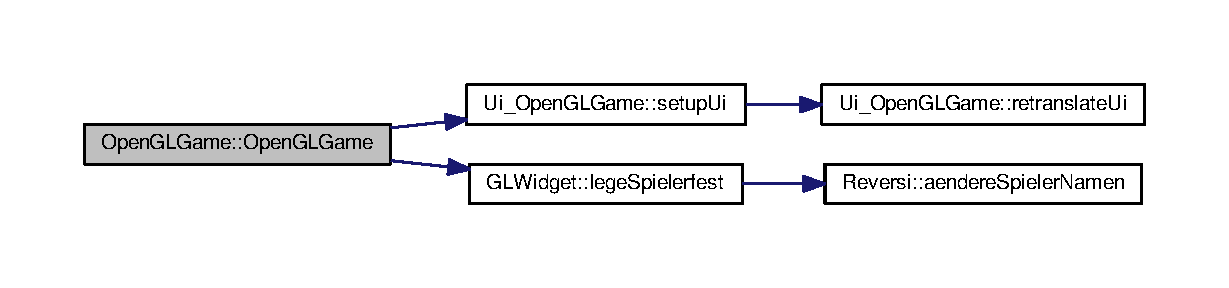
\includegraphics[width=350pt]{classOpenGLGame_a9082f6e7cad74cd49dab386bf14dc185_cgraph}
\end{center}
\end{figure}


\hypertarget{classOpenGLGame_a20705f1f3f495f65f2879681a20eb43b}{\index{Open\-G\-L\-Game@{Open\-G\-L\-Game}!$\sim$\-Open\-G\-L\-Game@{$\sim$\-Open\-G\-L\-Game}}
\index{$\sim$\-Open\-G\-L\-Game@{$\sim$\-Open\-G\-L\-Game}!OpenGLGame@{Open\-G\-L\-Game}}
\subsubsection[{$\sim$\-Open\-G\-L\-Game}]{\setlength{\rightskip}{0pt plus 5cm}Open\-G\-L\-Game\-::$\sim$\-Open\-G\-L\-Game (
\begin{DoxyParamCaption}
{}
\end{DoxyParamCaption}
)}}\label{classOpenGLGame_a20705f1f3f495f65f2879681a20eb43b}
Destruktor des Open\-G\-L\-Game-\/\-Objekts. 

The documentation for this class was generated from the following files\-:\begin{DoxyCompactItemize}
\item 
\hyperlink{openglgame_8h}{openglgame.\-h}\item 
\hyperlink{openglgame_8cpp}{openglgame.\-cpp}\end{DoxyCompactItemize}

\hypertarget{classUi_1_1OpenGLGame}{\section{Ui\-:\-:Open\-G\-L\-Game Class Reference}
\label{classUi_1_1OpenGLGame}\index{Ui\-::\-Open\-G\-L\-Game@{Ui\-::\-Open\-G\-L\-Game}}
}


{\ttfamily \#include $<$ui\-\_\-openglgame.\-h$>$}



Inheritance diagram for Ui\-:\-:Open\-G\-L\-Game\-:\nopagebreak
\begin{figure}[H]
\begin{center}
\leavevmode
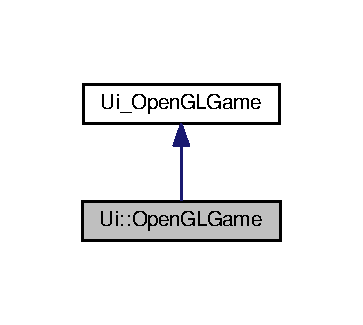
\includegraphics[width=174pt]{classUi_1_1OpenGLGame__inherit__graph}
\end{center}
\end{figure}


Collaboration diagram for Ui\-:\-:Open\-G\-L\-Game\-:\nopagebreak
\begin{figure}[H]
\begin{center}
\leavevmode
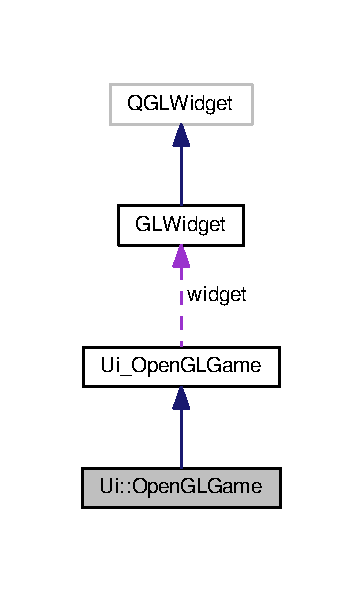
\includegraphics[width=174pt]{classUi_1_1OpenGLGame__coll__graph}
\end{center}
\end{figure}
\subsection*{Additional Inherited Members}


The documentation for this class was generated from the following file\-:\begin{DoxyCompactItemize}
\item 
\hyperlink{ui__openglgame_8h}{ui\-\_\-openglgame.\-h}\end{DoxyCompactItemize}

\hypertarget{classReversi}{\section{Reversi Class Reference}
\label{classReversi}\index{Reversi@{Reversi}}
}


{\ttfamily \#include $<$reversi.\-h$>$}



Inheritance diagram for Reversi\-:\nopagebreak
\begin{figure}[H]
\begin{center}
\leavevmode
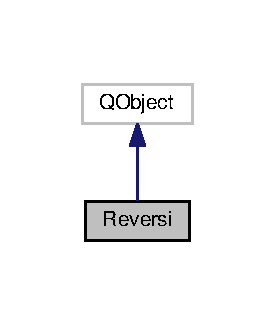
\includegraphics[width=132pt]{classReversi__inherit__graph}
\end{center}
\end{figure}


Collaboration diagram for Reversi\-:\nopagebreak
\begin{figure}[H]
\begin{center}
\leavevmode
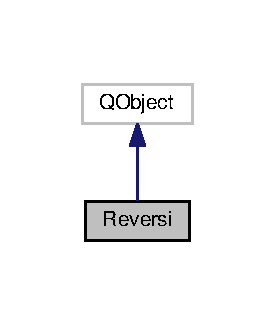
\includegraphics[width=132pt]{classReversi__coll__graph}
\end{center}
\end{figure}
\subsection*{Public Slots}
\begin{DoxyCompactItemize}
\item 
void \hyperlink{classReversi_a87d94f3c3325867453b5008b45829bd8}{setze\-Spielstein} (int angabe\-X, int angabe\-Y)
\item 
void \hyperlink{classReversi_a3e8988d0d227389d09673d4b5968a922}{next\-Turn} ()
\end{DoxyCompactItemize}
\subsection*{Signals}
\begin{DoxyCompactItemize}
\item 
void \hyperlink{classReversi_a23b22c8f180004e0df26478219bd9b93}{spiel\-Veraenderung} ()
\item 
void \hyperlink{classReversi_a619606ac8e7e930a5701d6f44730771c}{spiel\-Ende} (Q\-String gewinner\-Name)
\item 
void \hyperlink{classReversi_ad4baa37d88dbe7b4ddd8791943137537}{local\-Move} ()
\end{DoxyCompactItemize}
\subsection*{Public Member Functions}
\begin{DoxyCompactItemize}
\item 
\hyperlink{classReversi_a3a9ba93d8fa9ca6eb84c6a80e3068fac}{Reversi} (Q\-String spieler\-Name1=\char`\"{}Spieler 1\char`\"{}, Q\-String spieler\-Name2=\char`\"{}Spieler 2\char`\"{})
\item 
\hyperlink{classReversi_afd006e4fdacdedc4a3bb34fe6f1d1940}{$\sim$\-Reversi} ()
\item 
void \hyperlink{classReversi_a9606774d86257a0eee737fdd19d396dc}{start} ()
\item 
\hyperlink{classSpielbrett}{Spielbrett} $\ast$ \hyperlink{classReversi_af2c9e7f784cdd40097fdb81debc69c0a}{liefere\-Spielbrett} ()
\item 
\hyperlink{classSpieler}{Spieler} $\ast$ \hyperlink{classReversi_ac34759e93dc42daeadc694c7f438161f}{liefere\-Spieler} (int angabe\-I\-D)
\item 
\hyperlink{classSpieler}{Spieler} $\ast$$\ast$ \hyperlink{classReversi_a3473c04b4663baa9b9731e9b9cd8c09f}{liefere\-Alle\-Spieler} ()
\item 
vector$<$ \hyperlink{classSpielzug}{Spielzug} $>$ \hyperlink{classReversi_a552ef8aea3cadce41ed8de8c610eb795}{liefere\-Spielzuege} ()
\item 
vector$<$ \hyperlink{classSpielzug}{Spielzug} $>$ \hyperlink{classReversi_a0e0285172b42340b0dc90837840f19c2}{liefere\-Erlaubte\-Spielzuege} ()
\item 
int \hyperlink{classReversi_a7ab1778f35a7335ab8522d81610e8d1f}{liefere\-Aktuellen\-Spieler} ()
\item 
void \hyperlink{classReversi_ad6befc3b432e95f5afb11e1cd8890225}{aendere\-Spieler\-Namen} (Q\-String spieler1\-Name, Q\-String spieler2\-Name)
\end{DoxyCompactItemize}


\subsection{Detailed Description}
Diese Klasse repraesentiert das Reversi-\/\-Spiel. 

\subsection{Constructor \& Destructor Documentation}
\hypertarget{classReversi_a3a9ba93d8fa9ca6eb84c6a80e3068fac}{\index{Reversi@{Reversi}!Reversi@{Reversi}}
\index{Reversi@{Reversi}!Reversi@{Reversi}}
\subsubsection[{Reversi}]{\setlength{\rightskip}{0pt plus 5cm}Reversi\-::\-Reversi (
\begin{DoxyParamCaption}
\item[{Q\-String}]{spieler\-Name1 = {\ttfamily \char`\"{}Spieler~1\char`\"{}}, }
\item[{Q\-String}]{spieler\-Name2 = {\ttfamily \char`\"{}Spieler~2\char`\"{}}}
\end{DoxyParamCaption}
)}}\label{classReversi_a3a9ba93d8fa9ca6eb84c6a80e3068fac}
Konstruiert ein Objekt vom Typ \hyperlink{classReversi}{Reversi} mit Hilfe der Angabe der beiden Spielernamen. Dabei werden alle Reversi-\/\-Start Optionen festgelegt. z.\-B. Erlaubte Spielzuege der beiden \hyperlink{classSpieler}{Spieler}, sowie die Namen und Anzahl der Spielzuege etc...


\begin{DoxyParams}{Parameters}
{\em spieler\-Name1} & \\
\hline
{\em spieler\-Name2} & \\
\hline
\end{DoxyParams}
\hypertarget{classReversi_afd006e4fdacdedc4a3bb34fe6f1d1940}{\index{Reversi@{Reversi}!$\sim$\-Reversi@{$\sim$\-Reversi}}
\index{$\sim$\-Reversi@{$\sim$\-Reversi}!Reversi@{Reversi}}
\subsubsection[{$\sim$\-Reversi}]{\setlength{\rightskip}{0pt plus 5cm}Reversi\-::$\sim$\-Reversi (
\begin{DoxyParamCaption}
{}
\end{DoxyParamCaption}
)}}\label{classReversi_afd006e4fdacdedc4a3bb34fe6f1d1940}
Destruktor fuer die Reversi-\/\-Klasse. 

\subsection{Member Function Documentation}
\hypertarget{classReversi_ad6befc3b432e95f5afb11e1cd8890225}{\index{Reversi@{Reversi}!aendere\-Spieler\-Namen@{aendere\-Spieler\-Namen}}
\index{aendere\-Spieler\-Namen@{aendere\-Spieler\-Namen}!Reversi@{Reversi}}
\subsubsection[{aendere\-Spieler\-Namen}]{\setlength{\rightskip}{0pt plus 5cm}void Reversi\-::aendere\-Spieler\-Namen (
\begin{DoxyParamCaption}
\item[{Q\-String}]{spieler1\-Name, }
\item[{Q\-String}]{spieler2\-Name}
\end{DoxyParamCaption}
)}}\label{classReversi_ad6befc3b432e95f5afb11e1cd8890225}
Aendert die Namen beider \hyperlink{classSpieler}{Spieler}, mit der Hilfe der Angabe der neuen Spielernamen.


\begin{DoxyParams}{Parameters}
{\em spieler1\-Name} & Die Angabe des Spielernamens. \\
\hline
{\em spieler2\-Name} & Die Angabe des Spielernamens. \\
\hline
\end{DoxyParams}
\hypertarget{classReversi_a7ab1778f35a7335ab8522d81610e8d1f}{\index{Reversi@{Reversi}!liefere\-Aktuellen\-Spieler@{liefere\-Aktuellen\-Spieler}}
\index{liefere\-Aktuellen\-Spieler@{liefere\-Aktuellen\-Spieler}!Reversi@{Reversi}}
\subsubsection[{liefere\-Aktuellen\-Spieler}]{\setlength{\rightskip}{0pt plus 5cm}int Reversi\-::liefere\-Aktuellen\-Spieler (
\begin{DoxyParamCaption}
{}
\end{DoxyParamCaption}
)}}\label{classReversi_a7ab1778f35a7335ab8522d81610e8d1f}
Liefert den aktuellen \hyperlink{classSpieler}{Spieler} als I\-D.

\begin{DoxyReturn}{Returns}
Die I\-D des aktuellen Spielers. 
\end{DoxyReturn}
\hypertarget{classReversi_a3473c04b4663baa9b9731e9b9cd8c09f}{\index{Reversi@{Reversi}!liefere\-Alle\-Spieler@{liefere\-Alle\-Spieler}}
\index{liefere\-Alle\-Spieler@{liefere\-Alle\-Spieler}!Reversi@{Reversi}}
\subsubsection[{liefere\-Alle\-Spieler}]{\setlength{\rightskip}{0pt plus 5cm}{\bf Spieler} $\ast$$\ast$ Reversi\-::liefere\-Alle\-Spieler (
\begin{DoxyParamCaption}
{}
\end{DoxyParamCaption}
)}}\label{classReversi_a3473c04b4663baa9b9731e9b9cd8c09f}
Liefert alle \hyperlink{classSpieler}{Spieler} des Spiels.

\begin{DoxyReturn}{Returns}
Alle \hyperlink{classSpieler}{Spieler} des Spiels. 
\end{DoxyReturn}
\hypertarget{classReversi_a0e0285172b42340b0dc90837840f19c2}{\index{Reversi@{Reversi}!liefere\-Erlaubte\-Spielzuege@{liefere\-Erlaubte\-Spielzuege}}
\index{liefere\-Erlaubte\-Spielzuege@{liefere\-Erlaubte\-Spielzuege}!Reversi@{Reversi}}
\subsubsection[{liefere\-Erlaubte\-Spielzuege}]{\setlength{\rightskip}{0pt plus 5cm}vector$<$ {\bf Spielzug} $>$ Reversi\-::liefere\-Erlaubte\-Spielzuege (
\begin{DoxyParamCaption}
{}
\end{DoxyParamCaption}
)}}\label{classReversi_a0e0285172b42340b0dc90837840f19c2}
Liefert die erlaubten Spielzuege.

\begin{DoxyReturn}{Returns}
Die erlaubten Spielzuege. 
\end{DoxyReturn}
\hypertarget{classReversi_af2c9e7f784cdd40097fdb81debc69c0a}{\index{Reversi@{Reversi}!liefere\-Spielbrett@{liefere\-Spielbrett}}
\index{liefere\-Spielbrett@{liefere\-Spielbrett}!Reversi@{Reversi}}
\subsubsection[{liefere\-Spielbrett}]{\setlength{\rightskip}{0pt plus 5cm}{\bf Spielbrett} $\ast$ Reversi\-::liefere\-Spielbrett (
\begin{DoxyParamCaption}
{}
\end{DoxyParamCaption}
)}}\label{classReversi_af2c9e7f784cdd40097fdb81debc69c0a}
Liefert das Spielfeld-\/\-Objekt.

\begin{DoxyReturn}{Returns}
Das Spielfeld-\/\-Objekt. 
\end{DoxyReturn}
\hypertarget{classReversi_ac34759e93dc42daeadc694c7f438161f}{\index{Reversi@{Reversi}!liefere\-Spieler@{liefere\-Spieler}}
\index{liefere\-Spieler@{liefere\-Spieler}!Reversi@{Reversi}}
\subsubsection[{liefere\-Spieler}]{\setlength{\rightskip}{0pt plus 5cm}{\bf Spieler} $\ast$ Reversi\-::liefere\-Spieler (
\begin{DoxyParamCaption}
\item[{int}]{angabe\-I\-D}
\end{DoxyParamCaption}
)}}\label{classReversi_ac34759e93dc42daeadc694c7f438161f}
Liefert den einen \hyperlink{classSpieler}{Spieler}, mit Hilfe der Angabe seiner I\-D.


\begin{DoxyParams}{Parameters}
{\em angabe\-I\-D} & Die Angabe der I\-D des Spielers. \\
\hline
\end{DoxyParams}
\begin{DoxyReturn}{Returns}
\hyperlink{classSpieler}{Spieler}, mit angegebener I\-D. 
\end{DoxyReturn}
\hypertarget{classReversi_a552ef8aea3cadce41ed8de8c610eb795}{\index{Reversi@{Reversi}!liefere\-Spielzuege@{liefere\-Spielzuege}}
\index{liefere\-Spielzuege@{liefere\-Spielzuege}!Reversi@{Reversi}}
\subsubsection[{liefere\-Spielzuege}]{\setlength{\rightskip}{0pt plus 5cm}vector$<$ {\bf Spielzug} $>$ Reversi\-::liefere\-Spielzuege (
\begin{DoxyParamCaption}
{}
\end{DoxyParamCaption}
)}}\label{classReversi_a552ef8aea3cadce41ed8de8c610eb795}
Liefert allegetaetigten Spielzuege.

\begin{DoxyReturn}{Returns}
Alle getaetigten Spielzuege. 
\end{DoxyReturn}
\hypertarget{classReversi_ad4baa37d88dbe7b4ddd8791943137537}{\index{Reversi@{Reversi}!local\-Move@{local\-Move}}
\index{local\-Move@{local\-Move}!Reversi@{Reversi}}
\subsubsection[{local\-Move}]{\setlength{\rightskip}{0pt plus 5cm}void Reversi\-::local\-Move (
\begin{DoxyParamCaption}
{}
\end{DoxyParamCaption}
)\hspace{0.3cm}{\ttfamily [signal]}}}\label{classReversi_ad4baa37d88dbe7b4ddd8791943137537}
Sendet ein Signal, wenn ein \hyperlink{classSpielzug}{Spielzug} akzeptiert wurde. \hypertarget{classReversi_a3e8988d0d227389d09673d4b5968a922}{\index{Reversi@{Reversi}!next\-Turn@{next\-Turn}}
\index{next\-Turn@{next\-Turn}!Reversi@{Reversi}}
\subsubsection[{next\-Turn}]{\setlength{\rightskip}{0pt plus 5cm}void Reversi\-::next\-Turn (
\begin{DoxyParamCaption}
{}
\end{DoxyParamCaption}
)\hspace{0.3cm}{\ttfamily [slot]}}}\label{classReversi_a3e8988d0d227389d09673d4b5968a922}
Prueft das Spiel auf ein Ende. Wenn dieses nicht erreicht ist, wird der naechste Zug eingeleitet. \hypertarget{classReversi_a87d94f3c3325867453b5008b45829bd8}{\index{Reversi@{Reversi}!setze\-Spielstein@{setze\-Spielstein}}
\index{setze\-Spielstein@{setze\-Spielstein}!Reversi@{Reversi}}
\subsubsection[{setze\-Spielstein}]{\setlength{\rightskip}{0pt plus 5cm}void Reversi\-::setze\-Spielstein (
\begin{DoxyParamCaption}
\item[{int}]{angabe\-X, }
\item[{int}]{angabe\-Y}
\end{DoxyParamCaption}
)\hspace{0.3cm}{\ttfamily [slot]}}}\label{classReversi_a87d94f3c3325867453b5008b45829bd8}
Setzt einen Spielstein auf das \hyperlink{classSpielbrett}{Spielbrett}.


\begin{DoxyParams}{Parameters}
{\em angabe\-X} & Die Angabe der X-\/\-Koordinate. \\
\hline
{\em angabe\-Y} & Die Angabe der Y-\/\-Koordinate. \\
\hline
\end{DoxyParams}
\hypertarget{classReversi_a619606ac8e7e930a5701d6f44730771c}{\index{Reversi@{Reversi}!spiel\-Ende@{spiel\-Ende}}
\index{spiel\-Ende@{spiel\-Ende}!Reversi@{Reversi}}
\subsubsection[{spiel\-Ende}]{\setlength{\rightskip}{0pt plus 5cm}void Reversi\-::spiel\-Ende (
\begin{DoxyParamCaption}
\item[{Q\-String}]{gewinner\-Name}
\end{DoxyParamCaption}
)\hspace{0.3cm}{\ttfamily [signal]}}}\label{classReversi_a619606ac8e7e930a5701d6f44730771c}
Sendet ein Signal wenn das Spiel zuende ist. \hypertarget{classReversi_a23b22c8f180004e0df26478219bd9b93}{\index{Reversi@{Reversi}!spiel\-Veraenderung@{spiel\-Veraenderung}}
\index{spiel\-Veraenderung@{spiel\-Veraenderung}!Reversi@{Reversi}}
\subsubsection[{spiel\-Veraenderung}]{\setlength{\rightskip}{0pt plus 5cm}void Reversi\-::spiel\-Veraenderung (
\begin{DoxyParamCaption}
{}
\end{DoxyParamCaption}
)\hspace{0.3cm}{\ttfamily [signal]}}}\label{classReversi_a23b22c8f180004e0df26478219bd9b93}
Sendet ein Signal, wenn sich an dem Spiel eine Veraendeung ergibt. \hypertarget{classReversi_a9606774d86257a0eee737fdd19d396dc}{\index{Reversi@{Reversi}!start@{start}}
\index{start@{start}!Reversi@{Reversi}}
\subsubsection[{start}]{\setlength{\rightskip}{0pt plus 5cm}void Reversi\-::start (
\begin{DoxyParamCaption}
{}
\end{DoxyParamCaption}
)}}\label{classReversi_a9606774d86257a0eee737fdd19d396dc}


The documentation for this class was generated from the following files\-:\begin{DoxyCompactItemize}
\item 
\hyperlink{reversi_8h}{reversi.\-h}\item 
\hyperlink{reversi_8cpp}{reversi.\-cpp}\end{DoxyCompactItemize}

\hypertarget{classSpielbrett}{\section{Spielbrett Class Reference}
\label{classSpielbrett}\index{Spielbrett@{Spielbrett}}
}


{\ttfamily \#include $<$spielbrett.\-h$>$}

\subsection*{Public Member Functions}
\begin{DoxyCompactItemize}
\item 
\hyperlink{classSpielbrett_ad1030668197b68a9db4626ae52fb5392}{Spielbrett} ()
\item 
bool \hyperlink{classSpielbrett_a1a4f79a33ee43258499cae2040093f46}{setze\-Spielstein} (\hyperlink{DEFINE_8h_af7777a498318335ea89b85bdc0d1651f}{Spieler\-Farbe} angabe\-Farbe, int angabe\-X, int angabe\-Y)
\item 
bool \hyperlink{classSpielbrett_ac8d008e1bd3471f99a5d25ceb1bf5caa}{setze\-Gueltigen\-Spielzug} (int angabe\-X, int angabe\-Y)
\item 
bool \hyperlink{classSpielbrett_a4ea6649406b8bc45ab9772b9f0a9f0a8}{drehe\-Spielstein} (int angabe\-X, int angabe\-Y)
\item 
void \hyperlink{classSpielbrett_aad45932000bdb82cc1c58c4dbce08045}{entferne\-Alle\-Drehungen} ()
\item 
void \hyperlink{classSpielbrett_a33d8b89cbb4266c522b950d58f180ad0}{entferne\-Alle\-Erlaubten\-Zuege} ()
\item 
void \hyperlink{classSpielbrett_ae561de28444766bf74705f7fc1d396f2}{setze\-Animation} (bool angabe\-Animation)
\item 
bool \hyperlink{classSpielbrett_a973e4e3f43906428d50479001c08aae5}{liefere\-Animation} ()
\item 
\hyperlink{DEFINE_8h_a38d3a135c8443ff29d22fa0756476c5b}{Feld\-Eigenschaft} \hyperlink{classSpielbrett_aa16a4e86f849602fd6868cc6772c46c2}{liefere\-Feldeigenschaft} (int angabe\-X, int angabe\-Y)
\item 
\hyperlink{DEFINE_8h_af7777a498318335ea89b85bdc0d1651f}{Spieler\-Farbe} \hyperlink{classSpielbrett_a361157137c7c7cda4e06f568131c8fc9}{liefere\-Farbe} (int angabe\-X, int angabe\-Y)
\item 
bool \hyperlink{classSpielbrett_a9ff04ceff05cfd689057788f8df4774f}{liefere\-Drehung} (int angabe\-X, int angabe\-Y)
\end{DoxyCompactItemize}


\subsection{Detailed Description}
Diese Klasse repraesentiert ein quadratisches \hyperlink{classSpielbrett}{Spielbrett}, welches aus 8 $\ast$ 8 quadratischen Feldern besteht. 

\subsection{Constructor \& Destructor Documentation}
\hypertarget{classSpielbrett_ad1030668197b68a9db4626ae52fb5392}{\index{Spielbrett@{Spielbrett}!Spielbrett@{Spielbrett}}
\index{Spielbrett@{Spielbrett}!Spielbrett@{Spielbrett}}
\subsubsection[{Spielbrett}]{\setlength{\rightskip}{0pt plus 5cm}Spielbrett\-::\-Spielbrett (
\begin{DoxyParamCaption}
{}
\end{DoxyParamCaption}
)}}\label{classSpielbrett_ad1030668197b68a9db4626ae52fb5392}
Konstruiert ein Objekt \hyperlink{classSpielbrett}{Spielbrett}, mit den Startoptionen von \hyperlink{classReversi}{Reversi}. 

\subsection{Member Function Documentation}
\hypertarget{classSpielbrett_a4ea6649406b8bc45ab9772b9f0a9f0a8}{\index{Spielbrett@{Spielbrett}!drehe\-Spielstein@{drehe\-Spielstein}}
\index{drehe\-Spielstein@{drehe\-Spielstein}!Spielbrett@{Spielbrett}}
\subsubsection[{drehe\-Spielstein}]{\setlength{\rightskip}{0pt plus 5cm}bool Spielbrett\-::drehe\-Spielstein (
\begin{DoxyParamCaption}
\item[{int}]{angabe\-X, }
\item[{int}]{angabe\-Y}
\end{DoxyParamCaption}
)}}\label{classSpielbrett_a4ea6649406b8bc45ab9772b9f0a9f0a8}
Wechselt mit der Hilfe der Angabe von X-\/ und Y-\/\-Koordinate die Farbe eines Spielsteins.


\begin{DoxyParams}{Parameters}
{\em angabe\-X} & Angabe der X-\/\-Koordinate. \\
\hline
{\em angabe\-Y} & Angabe der Y-\/\-Koordinate. \\
\hline
\end{DoxyParams}
\begin{DoxyReturn}{Returns}
True wenn erfolgreich $\vert$ False wenn nicht moeglich. 
\end{DoxyReturn}


Here is the call graph for this function\-:\nopagebreak
\begin{figure}[H]
\begin{center}
\leavevmode
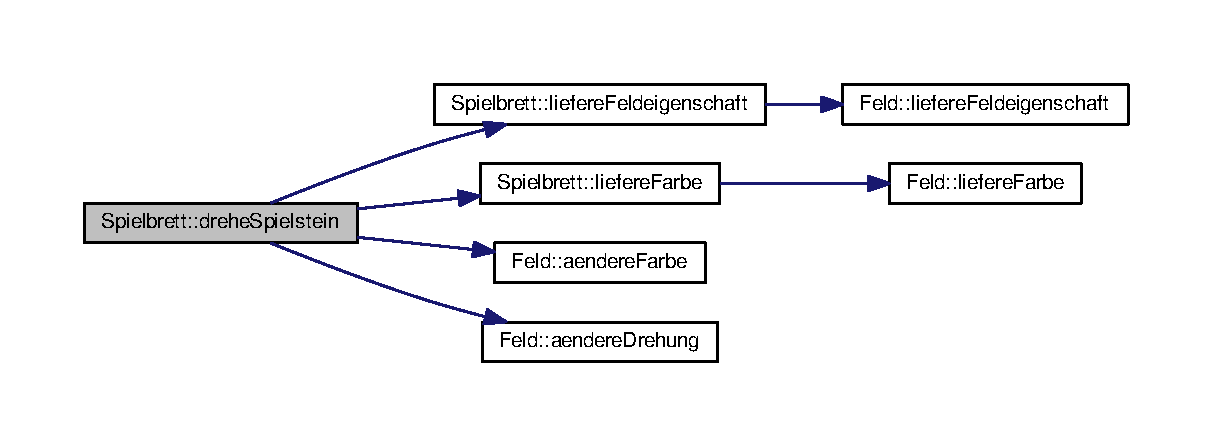
\includegraphics[width=350pt]{classSpielbrett_a4ea6649406b8bc45ab9772b9f0a9f0a8_cgraph}
\end{center}
\end{figure}


\hypertarget{classSpielbrett_aad45932000bdb82cc1c58c4dbce08045}{\index{Spielbrett@{Spielbrett}!entferne\-Alle\-Drehungen@{entferne\-Alle\-Drehungen}}
\index{entferne\-Alle\-Drehungen@{entferne\-Alle\-Drehungen}!Spielbrett@{Spielbrett}}
\subsubsection[{entferne\-Alle\-Drehungen}]{\setlength{\rightskip}{0pt plus 5cm}void Spielbrett\-::entferne\-Alle\-Drehungen (
\begin{DoxyParamCaption}
{}
\end{DoxyParamCaption}
)}}\label{classSpielbrett_aad45932000bdb82cc1c58c4dbce08045}
Entfernt alle festgelegten Drehungen aller Spielfelder des Spielbretts. 

Here is the call graph for this function\-:\nopagebreak
\begin{figure}[H]
\begin{center}
\leavevmode
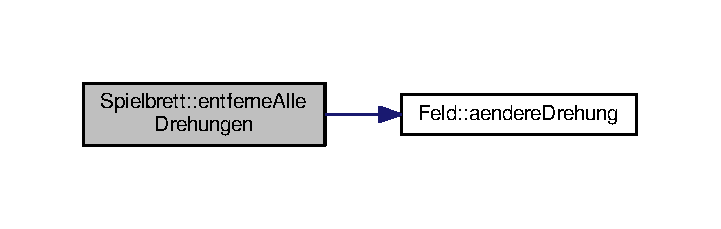
\includegraphics[width=346pt]{classSpielbrett_aad45932000bdb82cc1c58c4dbce08045_cgraph}
\end{center}
\end{figure}


\hypertarget{classSpielbrett_a33d8b89cbb4266c522b950d58f180ad0}{\index{Spielbrett@{Spielbrett}!entferne\-Alle\-Erlaubten\-Zuege@{entferne\-Alle\-Erlaubten\-Zuege}}
\index{entferne\-Alle\-Erlaubten\-Zuege@{entferne\-Alle\-Erlaubten\-Zuege}!Spielbrett@{Spielbrett}}
\subsubsection[{entferne\-Alle\-Erlaubten\-Zuege}]{\setlength{\rightskip}{0pt plus 5cm}void Spielbrett\-::entferne\-Alle\-Erlaubten\-Zuege (
\begin{DoxyParamCaption}
{}
\end{DoxyParamCaption}
)}}\label{classSpielbrett_a33d8b89cbb4266c522b950d58f180ad0}
Entfernt alle erlaubten Spielzuege von den einzelnen Spielfeldern und ersetzt diese durch \char`\"{}leer\char`\"{}. 

Here is the call graph for this function\-:\nopagebreak
\begin{figure}[H]
\begin{center}
\leavevmode
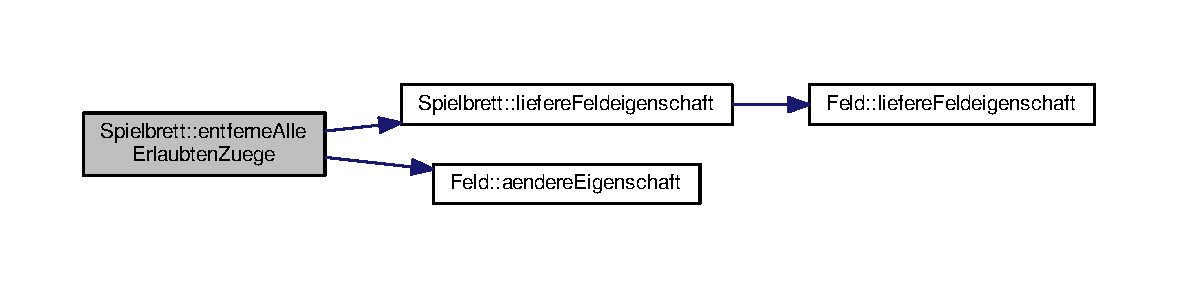
\includegraphics[width=350pt]{classSpielbrett_a33d8b89cbb4266c522b950d58f180ad0_cgraph}
\end{center}
\end{figure}


\hypertarget{classSpielbrett_a973e4e3f43906428d50479001c08aae5}{\index{Spielbrett@{Spielbrett}!liefere\-Animation@{liefere\-Animation}}
\index{liefere\-Animation@{liefere\-Animation}!Spielbrett@{Spielbrett}}
\subsubsection[{liefere\-Animation}]{\setlength{\rightskip}{0pt plus 5cm}bool Spielbrett\-::liefere\-Animation (
\begin{DoxyParamCaption}
{}
\end{DoxyParamCaption}
)}}\label{classSpielbrett_a973e4e3f43906428d50479001c08aae5}
Liefert die Animation(boolscher Wert) des Spielbretts.

\begin{DoxyReturn}{Returns}
Die Animation des Spielbretts als bool. 
\end{DoxyReturn}
\hypertarget{classSpielbrett_a9ff04ceff05cfd689057788f8df4774f}{\index{Spielbrett@{Spielbrett}!liefere\-Drehung@{liefere\-Drehung}}
\index{liefere\-Drehung@{liefere\-Drehung}!Spielbrett@{Spielbrett}}
\subsubsection[{liefere\-Drehung}]{\setlength{\rightskip}{0pt plus 5cm}bool Spielbrett\-::liefere\-Drehung (
\begin{DoxyParamCaption}
\item[{int}]{angabe\-X, }
\item[{int}]{angabe\-Y}
\end{DoxyParamCaption}
)}}\label{classSpielbrett_a9ff04ceff05cfd689057788f8df4774f}
Liefert die Drehung(ob der Stein an dieser Position gedreht wird) eines Feldes auf dem \hyperlink{classSpielbrett}{Spielbrett}.


\begin{DoxyParams}{Parameters}
{\em angabe\-X} & Die Angabe der X-\/\-Koordinate. \\
\hline
{\em angabe\-Y} & Die Angabe der Y-\/\-Koordinate. \\
\hline
\end{DoxyParams}
\begin{DoxyReturn}{Returns}
Die Drehung des Feldes mit der Position von X und Y. 
\end{DoxyReturn}


Here is the call graph for this function\-:\nopagebreak
\begin{figure}[H]
\begin{center}
\leavevmode
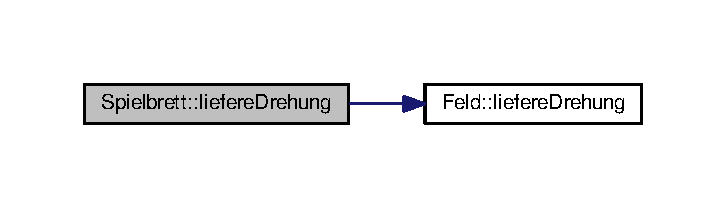
\includegraphics[width=348pt]{classSpielbrett_a9ff04ceff05cfd689057788f8df4774f_cgraph}
\end{center}
\end{figure}


\hypertarget{classSpielbrett_a361157137c7c7cda4e06f568131c8fc9}{\index{Spielbrett@{Spielbrett}!liefere\-Farbe@{liefere\-Farbe}}
\index{liefere\-Farbe@{liefere\-Farbe}!Spielbrett@{Spielbrett}}
\subsubsection[{liefere\-Farbe}]{\setlength{\rightskip}{0pt plus 5cm}{\bf Spieler\-Farbe} Spielbrett\-::liefere\-Farbe (
\begin{DoxyParamCaption}
\item[{int}]{angabe\-X, }
\item[{int}]{angabe\-Y}
\end{DoxyParamCaption}
)}}\label{classSpielbrett_a361157137c7c7cda4e06f568131c8fc9}
Liefert die Farbe eines Feldes auf dem \hyperlink{classSpielbrett}{Spielbrett}.


\begin{DoxyParams}{Parameters}
{\em angabe\-X} & Die Angabe der X-\/\-Koordinate. \\
\hline
{\em angabe\-Y} & Die Angabe der Y-\/\-Koordinate. \\
\hline
\end{DoxyParams}
\begin{DoxyReturn}{Returns}
Die Farbe des Feldes mit der Position von X und Y. 
\end{DoxyReturn}


Here is the call graph for this function\-:\nopagebreak
\begin{figure}[H]
\begin{center}
\leavevmode
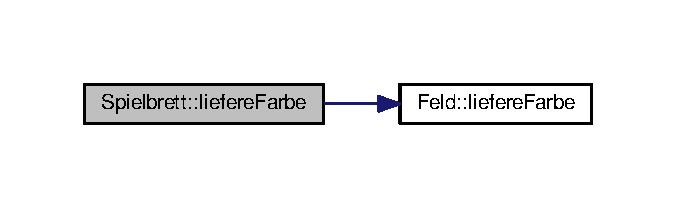
\includegraphics[width=324pt]{classSpielbrett_a361157137c7c7cda4e06f568131c8fc9_cgraph}
\end{center}
\end{figure}


\hypertarget{classSpielbrett_aa16a4e86f849602fd6868cc6772c46c2}{\index{Spielbrett@{Spielbrett}!liefere\-Feldeigenschaft@{liefere\-Feldeigenschaft}}
\index{liefere\-Feldeigenschaft@{liefere\-Feldeigenschaft}!Spielbrett@{Spielbrett}}
\subsubsection[{liefere\-Feldeigenschaft}]{\setlength{\rightskip}{0pt plus 5cm}{\bf Feld\-Eigenschaft} Spielbrett\-::liefere\-Feldeigenschaft (
\begin{DoxyParamCaption}
\item[{int}]{angabe\-X, }
\item[{int}]{angabe\-Y}
\end{DoxyParamCaption}
)}}\label{classSpielbrett_aa16a4e86f849602fd6868cc6772c46c2}
Liefert die Eigenschaft eines Feldes auf dem \hyperlink{classSpielbrett}{Spielbrett}.


\begin{DoxyParams}{Parameters}
{\em angabe\-X} & Die Angabe der X-\/\-Koordinate. \\
\hline
{\em angabe\-Y} & Die Angabe der Y-\/\-Koordinate. \\
\hline
\end{DoxyParams}
\begin{DoxyReturn}{Returns}
Die Feldeigenschaft des Feldes mit der Position von X und Y. 
\end{DoxyReturn}


Here is the call graph for this function\-:\nopagebreak
\begin{figure}[H]
\begin{center}
\leavevmode
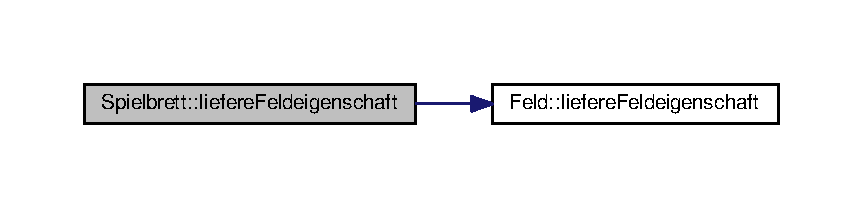
\includegraphics[width=350pt]{classSpielbrett_aa16a4e86f849602fd6868cc6772c46c2_cgraph}
\end{center}
\end{figure}


\hypertarget{classSpielbrett_ae561de28444766bf74705f7fc1d396f2}{\index{Spielbrett@{Spielbrett}!setze\-Animation@{setze\-Animation}}
\index{setze\-Animation@{setze\-Animation}!Spielbrett@{Spielbrett}}
\subsubsection[{setze\-Animation}]{\setlength{\rightskip}{0pt plus 5cm}void Spielbrett\-::setze\-Animation (
\begin{DoxyParamCaption}
\item[{bool}]{angabe\-Animation}
\end{DoxyParamCaption}
)}}\label{classSpielbrett_ae561de28444766bf74705f7fc1d396f2}
Setzt die Animation des Spielbretts.


\begin{DoxyParams}{Parameters}
{\em angabe\-Animation} & Angabe der Animation als boolschen Wert. \\
\hline
\end{DoxyParams}
\hypertarget{classSpielbrett_ac8d008e1bd3471f99a5d25ceb1bf5caa}{\index{Spielbrett@{Spielbrett}!setze\-Gueltigen\-Spielzug@{setze\-Gueltigen\-Spielzug}}
\index{setze\-Gueltigen\-Spielzug@{setze\-Gueltigen\-Spielzug}!Spielbrett@{Spielbrett}}
\subsubsection[{setze\-Gueltigen\-Spielzug}]{\setlength{\rightskip}{0pt plus 5cm}bool Spielbrett\-::setze\-Gueltigen\-Spielzug (
\begin{DoxyParamCaption}
\item[{int}]{angabe\-X, }
\item[{int}]{angabe\-Y}
\end{DoxyParamCaption}
)}}\label{classSpielbrett_ac8d008e1bd3471f99a5d25ceb1bf5caa}
Setzt mit der Hilfe der Angabe von X-\/ und Y-\/\-Koordinate einen gueltigen \hyperlink{classSpielzug}{Spielzug} fest.


\begin{DoxyParams}{Parameters}
{\em angabe\-X} & Angabe der X-\/\-Koordinate. \\
\hline
{\em angabe\-Y} & Angabe der Y-\/\-Koordinate. \\
\hline
\end{DoxyParams}
\begin{DoxyReturn}{Returns}
True wenn erfolgreich festgelegt $\vert$ False wenn nicht moeglich. 
\end{DoxyReturn}


Here is the call graph for this function\-:\nopagebreak
\begin{figure}[H]
\begin{center}
\leavevmode
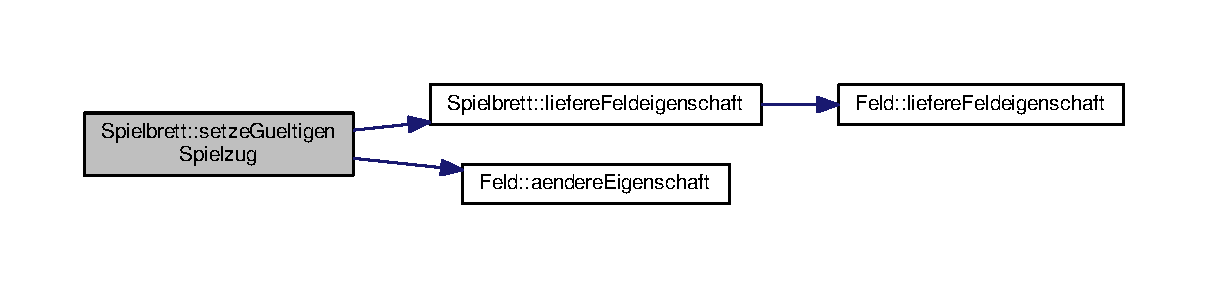
\includegraphics[width=350pt]{classSpielbrett_ac8d008e1bd3471f99a5d25ceb1bf5caa_cgraph}
\end{center}
\end{figure}


\hypertarget{classSpielbrett_a1a4f79a33ee43258499cae2040093f46}{\index{Spielbrett@{Spielbrett}!setze\-Spielstein@{setze\-Spielstein}}
\index{setze\-Spielstein@{setze\-Spielstein}!Spielbrett@{Spielbrett}}
\subsubsection[{setze\-Spielstein}]{\setlength{\rightskip}{0pt plus 5cm}bool Spielbrett\-::setze\-Spielstein (
\begin{DoxyParamCaption}
\item[{{\bf Spieler\-Farbe}}]{angabe\-Farbe, }
\item[{int}]{angabe\-X, }
\item[{int}]{angabe\-Y}
\end{DoxyParamCaption}
)}}\label{classSpielbrett_a1a4f79a33ee43258499cae2040093f46}
Setzt einen Spielstein an eine Position des Spielbretts. 
\begin{DoxyParams}{Parameters}
{\em angabe\-Farbe} & Angabe der Farbe des Spielsteins. \\
\hline
{\em angabe\-X} & Angabe der X-\/\-Koordinate. \\
\hline
{\em angabe\-Y} & Angabe der Y-\/\-Koordinate. \\
\hline
\end{DoxyParams}
\begin{DoxyReturn}{Returns}
True wenn setzten erfolgreich $\vert$ False wenn nicht erlaubt. 
\end{DoxyReturn}


Here is the call graph for this function\-:\nopagebreak
\begin{figure}[H]
\begin{center}
\leavevmode
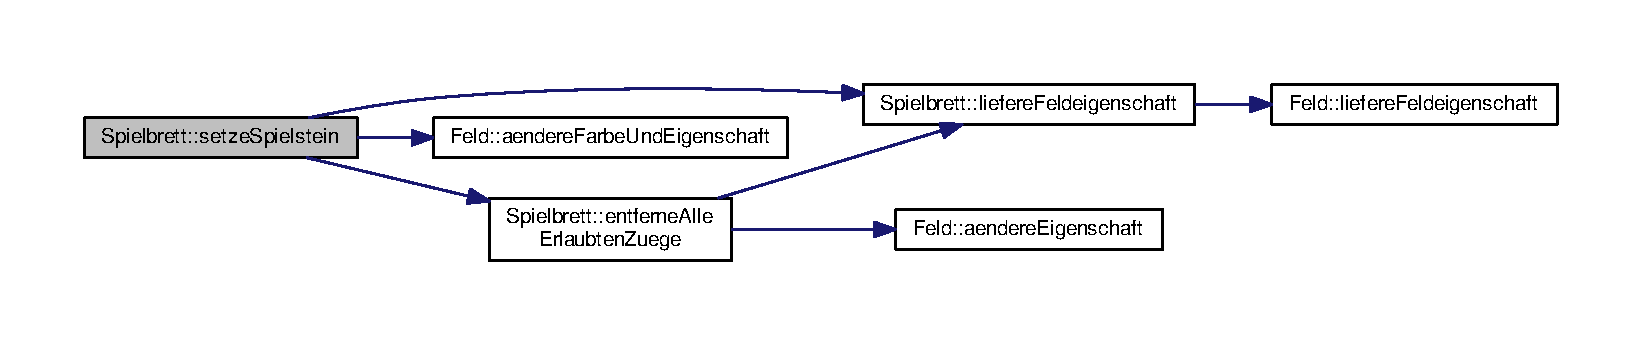
\includegraphics[width=350pt]{classSpielbrett_a1a4f79a33ee43258499cae2040093f46_cgraph}
\end{center}
\end{figure}




The documentation for this class was generated from the following files\-:\begin{DoxyCompactItemize}
\item 
\hyperlink{spielbrett_8h}{spielbrett.\-h}\item 
\hyperlink{spielbrett_8cpp}{spielbrett.\-cpp}\end{DoxyCompactItemize}

\hypertarget{classSpieler}{\section{Spieler Class Reference}
\label{classSpieler}\index{Spieler@{Spieler}}
}


{\ttfamily \#include $<$spieler.\-h$>$}

\subsection*{Public Member Functions}
\begin{DoxyCompactItemize}
\item 
\hyperlink{classSpieler_aa7e36bd9766673980d37fc93514b709c}{Spieler} (int angabe\-I\-D, Q\-String angabe\-Name, \hyperlink{DEFINE_8h_af7777a498318335ea89b85bdc0d1651f}{Spieler\-Farbe} angabe\-Farbe)
\item 
Q\-String \hyperlink{classSpieler_ab98f6cd34355abdbacfe90fd4f29c828}{liefere\-Name} ()
\item 
int \hyperlink{classSpieler_a57b383a331cb0c483a98a0bd39d489fc}{liefere\-Spieler\-I\-D} ()
\item 
\hyperlink{DEFINE_8h_af7777a498318335ea89b85bdc0d1651f}{Spieler\-Farbe} \hyperlink{classSpieler_a215f804783a3ebb96a1ceda8ffb1fc32}{liefere\-Spieler\-Farbe} ()
\item 
int \hyperlink{classSpieler_a8f7175f91c3b27f2da17b6c2056fd78f}{liefere\-Punkte} ()
\item 
void \hyperlink{classSpieler_affffa216287f59762c812be82d291945}{setze\-Anzahl\-Zurueck} ()
\item 
void \hyperlink{classSpieler_a572ac9e1dc7ced68f7093d2a804c1795}{erhoehe\-Anzahl\-Erlaubt} ()
\item 
int \hyperlink{classSpieler_a4d911d9721c64bca5f50ef0424863517}{liefere\-Anzahl\-Erlaubt} ()
\item 
void \hyperlink{classSpieler_a7208f0e7168efad1dda334ef7f394092}{aendere\-Name} (Q\-String angabe\-Name)
\item 
void \hyperlink{classSpieler_a8429133e40c2cc08592748e96795b3b6}{aendere\-Punkte} (int angabe\-Punkte)
\item 
void \hyperlink{classSpieler_ad98ec95472e5dc130b5c436c98469171}{aendere\-Spieler\-Farbe} (\hyperlink{DEFINE_8h_af7777a498318335ea89b85bdc0d1651f}{Spieler\-Farbe} angabe\-Farbe)
\item 
void \hyperlink{classSpieler_a5e56b6bf328dd8bbc9df0305add0e5e6}{aendere\-Spieler\-I\-D} (int angabe\-I\-D)
\end{DoxyCompactItemize}


\subsection{Detailed Description}
Diese Klasse repraesentiert einen \hyperlink{classSpieler}{Spieler}. 

\subsection{Constructor \& Destructor Documentation}
\hypertarget{classSpieler_aa7e36bd9766673980d37fc93514b709c}{\index{Spieler@{Spieler}!Spieler@{Spieler}}
\index{Spieler@{Spieler}!Spieler@{Spieler}}
\subsubsection[{Spieler}]{\setlength{\rightskip}{0pt plus 5cm}Spieler\-::\-Spieler (
\begin{DoxyParamCaption}
\item[{int}]{angabe\-I\-D, }
\item[{Q\-String}]{angabe\-Name, }
\item[{{\bf Spieler\-Farbe}}]{angabe\-Farbe}
\end{DoxyParamCaption}
)}}\label{classSpieler_aa7e36bd9766673980d37fc93514b709c}
Konstruiert ein Objekt vom Typ \hyperlink{classSpieler}{Spieler} mit hilfe der Angabe von der Spieler\-I\-D, des Namens und der Spielerfarbe.


\begin{DoxyParams}{Parameters}
{\em angabe\-I\-D} & Die Spieler\-I\-D als Int-\/\-Wert. \\
\hline
{\em angabe\-Name} & Angabe des Spielernamens. \\
\hline
{\em angabe\-Farbe} & Angabe der Spielerfarbe. \\
\hline
\end{DoxyParams}


\subsection{Member Function Documentation}
\hypertarget{classSpieler_a7208f0e7168efad1dda334ef7f394092}{\index{Spieler@{Spieler}!aendere\-Name@{aendere\-Name}}
\index{aendere\-Name@{aendere\-Name}!Spieler@{Spieler}}
\subsubsection[{aendere\-Name}]{\setlength{\rightskip}{0pt plus 5cm}void Spieler\-::aendere\-Name (
\begin{DoxyParamCaption}
\item[{Q\-String}]{angabe\-Name}
\end{DoxyParamCaption}
)}}\label{classSpieler_a7208f0e7168efad1dda334ef7f394092}
Aendert den Namen des Spielers.


\begin{DoxyParams}{Parameters}
{\em angabe\-Name} & Der neue Name fuer den \hyperlink{classSpieler}{Spieler}. \\
\hline
\end{DoxyParams}
\hypertarget{classSpieler_a8429133e40c2cc08592748e96795b3b6}{\index{Spieler@{Spieler}!aendere\-Punkte@{aendere\-Punkte}}
\index{aendere\-Punkte@{aendere\-Punkte}!Spieler@{Spieler}}
\subsubsection[{aendere\-Punkte}]{\setlength{\rightskip}{0pt plus 5cm}void Spieler\-::aendere\-Punkte (
\begin{DoxyParamCaption}
\item[{int}]{angabe\-Punkte}
\end{DoxyParamCaption}
)}}\label{classSpieler_a8429133e40c2cc08592748e96795b3b6}
Aendert den Punktestand des Spielers.


\begin{DoxyParams}{Parameters}
{\em angabe\-Punkte} & Der neue Punktestand des Spielers. \\
\hline
\end{DoxyParams}
\hypertarget{classSpieler_ad98ec95472e5dc130b5c436c98469171}{\index{Spieler@{Spieler}!aendere\-Spieler\-Farbe@{aendere\-Spieler\-Farbe}}
\index{aendere\-Spieler\-Farbe@{aendere\-Spieler\-Farbe}!Spieler@{Spieler}}
\subsubsection[{aendere\-Spieler\-Farbe}]{\setlength{\rightskip}{0pt plus 5cm}void Spieler\-::aendere\-Spieler\-Farbe (
\begin{DoxyParamCaption}
\item[{{\bf Spieler\-Farbe}}]{angabe\-Farbe}
\end{DoxyParamCaption}
)}}\label{classSpieler_ad98ec95472e5dc130b5c436c98469171}
Aendert die Farbe des Spielers.


\begin{DoxyParams}{Parameters}
{\em angabe\-Farbe} & Die neue Spielerfarbe. \\
\hline
\end{DoxyParams}
\hypertarget{classSpieler_a5e56b6bf328dd8bbc9df0305add0e5e6}{\index{Spieler@{Spieler}!aendere\-Spieler\-I\-D@{aendere\-Spieler\-I\-D}}
\index{aendere\-Spieler\-I\-D@{aendere\-Spieler\-I\-D}!Spieler@{Spieler}}
\subsubsection[{aendere\-Spieler\-I\-D}]{\setlength{\rightskip}{0pt plus 5cm}void Spieler\-::aendere\-Spieler\-I\-D (
\begin{DoxyParamCaption}
\item[{int}]{angabe\-I\-D}
\end{DoxyParamCaption}
)}}\label{classSpieler_a5e56b6bf328dd8bbc9df0305add0e5e6}
Aendert die I\-D des Spielers.


\begin{DoxyParams}{Parameters}
{\em angabe\-I\-D} & Die neue I\-D des Spielers. \\
\hline
\end{DoxyParams}
\hypertarget{classSpieler_a572ac9e1dc7ced68f7093d2a804c1795}{\index{Spieler@{Spieler}!erhoehe\-Anzahl\-Erlaubt@{erhoehe\-Anzahl\-Erlaubt}}
\index{erhoehe\-Anzahl\-Erlaubt@{erhoehe\-Anzahl\-Erlaubt}!Spieler@{Spieler}}
\subsubsection[{erhoehe\-Anzahl\-Erlaubt}]{\setlength{\rightskip}{0pt plus 5cm}void Spieler\-::erhoehe\-Anzahl\-Erlaubt (
\begin{DoxyParamCaption}
{}
\end{DoxyParamCaption}
)}}\label{classSpieler_a572ac9e1dc7ced68f7093d2a804c1795}
Erhoeht die Anzahl der erlaubten Spielzuege um 1. \hypertarget{classSpieler_a4d911d9721c64bca5f50ef0424863517}{\index{Spieler@{Spieler}!liefere\-Anzahl\-Erlaubt@{liefere\-Anzahl\-Erlaubt}}
\index{liefere\-Anzahl\-Erlaubt@{liefere\-Anzahl\-Erlaubt}!Spieler@{Spieler}}
\subsubsection[{liefere\-Anzahl\-Erlaubt}]{\setlength{\rightskip}{0pt plus 5cm}int Spieler\-::liefere\-Anzahl\-Erlaubt (
\begin{DoxyParamCaption}
{}
\end{DoxyParamCaption}
)}}\label{classSpieler_a4d911d9721c64bca5f50ef0424863517}
Liefert die Anzahl der erlaubten Spielzuege als Int-\/\-Wert.

\begin{DoxyReturn}{Returns}
Die Anzahl der erlaubten Spielzuege als Int-\/\-Wert. 
\end{DoxyReturn}
\hypertarget{classSpieler_ab98f6cd34355abdbacfe90fd4f29c828}{\index{Spieler@{Spieler}!liefere\-Name@{liefere\-Name}}
\index{liefere\-Name@{liefere\-Name}!Spieler@{Spieler}}
\subsubsection[{liefere\-Name}]{\setlength{\rightskip}{0pt plus 5cm}Q\-String Spieler\-::liefere\-Name (
\begin{DoxyParamCaption}
{}
\end{DoxyParamCaption}
)}}\label{classSpieler_ab98f6cd34355abdbacfe90fd4f29c828}
Liefert den Namen des Spielers als Q\-String.

\begin{DoxyReturn}{Returns}
Den Namen des Spielers als Q\-String. 
\end{DoxyReturn}
\hypertarget{classSpieler_a8f7175f91c3b27f2da17b6c2056fd78f}{\index{Spieler@{Spieler}!liefere\-Punkte@{liefere\-Punkte}}
\index{liefere\-Punkte@{liefere\-Punkte}!Spieler@{Spieler}}
\subsubsection[{liefere\-Punkte}]{\setlength{\rightskip}{0pt plus 5cm}int Spieler\-::liefere\-Punkte (
\begin{DoxyParamCaption}
{}
\end{DoxyParamCaption}
)}}\label{classSpieler_a8f7175f91c3b27f2da17b6c2056fd78f}
Liefert den Punktestand des einzelnen Spielers als Int-\/\-Wert.

\begin{DoxyReturn}{Returns}
Liefert den Punktestand des Spielers als Int-\/\-Wert. 
\end{DoxyReturn}
\hypertarget{classSpieler_a215f804783a3ebb96a1ceda8ffb1fc32}{\index{Spieler@{Spieler}!liefere\-Spieler\-Farbe@{liefere\-Spieler\-Farbe}}
\index{liefere\-Spieler\-Farbe@{liefere\-Spieler\-Farbe}!Spieler@{Spieler}}
\subsubsection[{liefere\-Spieler\-Farbe}]{\setlength{\rightskip}{0pt plus 5cm}{\bf Spieler\-Farbe} Spieler\-::liefere\-Spieler\-Farbe (
\begin{DoxyParamCaption}
{}
\end{DoxyParamCaption}
)}}\label{classSpieler_a215f804783a3ebb96a1ceda8ffb1fc32}
Liefert die Farbe des Spielers.

\begin{DoxyReturn}{Returns}
Die Farbe des Spielers. 
\end{DoxyReturn}
\hypertarget{classSpieler_a57b383a331cb0c483a98a0bd39d489fc}{\index{Spieler@{Spieler}!liefere\-Spieler\-I\-D@{liefere\-Spieler\-I\-D}}
\index{liefere\-Spieler\-I\-D@{liefere\-Spieler\-I\-D}!Spieler@{Spieler}}
\subsubsection[{liefere\-Spieler\-I\-D}]{\setlength{\rightskip}{0pt plus 5cm}int Spieler\-::liefere\-Spieler\-I\-D (
\begin{DoxyParamCaption}
{}
\end{DoxyParamCaption}
)}}\label{classSpieler_a57b383a331cb0c483a98a0bd39d489fc}
Liefert die I\-D des Spielers als Int-\/\-Wert.

\begin{DoxyReturn}{Returns}
Die I\-D des Spielers als Int-\/\-Wert. 
\end{DoxyReturn}
\hypertarget{classSpieler_affffa216287f59762c812be82d291945}{\index{Spieler@{Spieler}!setze\-Anzahl\-Zurueck@{setze\-Anzahl\-Zurueck}}
\index{setze\-Anzahl\-Zurueck@{setze\-Anzahl\-Zurueck}!Spieler@{Spieler}}
\subsubsection[{setze\-Anzahl\-Zurueck}]{\setlength{\rightskip}{0pt plus 5cm}void Spieler\-::setze\-Anzahl\-Zurueck (
\begin{DoxyParamCaption}
{}
\end{DoxyParamCaption}
)}}\label{classSpieler_affffa216287f59762c812be82d291945}
Setzt die Anzahl der Spielzuege fuer diesen \hyperlink{classSpieler}{Spieler} auf 0. 

The documentation for this class was generated from the following files\-:\begin{DoxyCompactItemize}
\item 
\hyperlink{spieler_8h}{spieler.\-h}\item 
\hyperlink{spieler_8cpp}{spieler.\-cpp}\end{DoxyCompactItemize}

\hypertarget{classUi_1_1SpielLaden}{\section{Ui\-:\-:Spiel\-Laden Class Reference}
\label{classUi_1_1SpielLaden}\index{Ui\-::\-Spiel\-Laden@{Ui\-::\-Spiel\-Laden}}
}


{\ttfamily \#include $<$ui\-\_\-spielladen.\-h$>$}



Inheritance diagram for Ui\-:\-:Spiel\-Laden\-:\nopagebreak
\begin{figure}[H]
\begin{center}
\leavevmode
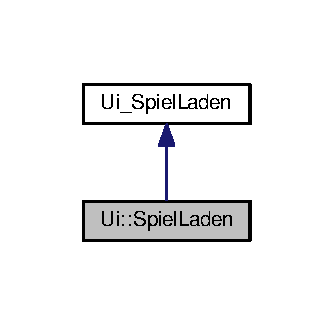
\includegraphics[width=160pt]{classUi_1_1SpielLaden__inherit__graph}
\end{center}
\end{figure}


Collaboration diagram for Ui\-:\-:Spiel\-Laden\-:\nopagebreak
\begin{figure}[H]
\begin{center}
\leavevmode
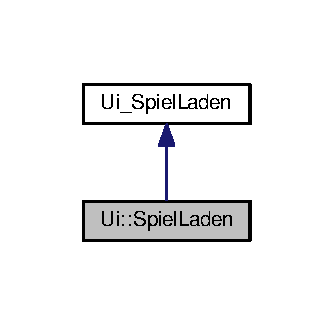
\includegraphics[width=160pt]{classUi_1_1SpielLaden__coll__graph}
\end{center}
\end{figure}
\subsection*{Additional Inherited Members}


The documentation for this class was generated from the following file\-:\begin{DoxyCompactItemize}
\item 
\hyperlink{ui__spielladen_8h}{ui\-\_\-spielladen.\-h}\end{DoxyCompactItemize}

\hypertarget{classSpielLaden}{\section{Spiel\-Laden Class Reference}
\label{classSpielLaden}\index{Spiel\-Laden@{Spiel\-Laden}}
}


{\ttfamily \#include $<$spielladen.\-h$>$}



Inheritance diagram for Spiel\-Laden\-:\nopagebreak
\begin{figure}[H]
\begin{center}
\leavevmode
\includegraphics[width=144pt]{classSpielLaden__inherit__graph}
\end{center}
\end{figure}


Collaboration diagram for Spiel\-Laden\-:\nopagebreak
\begin{figure}[H]
\begin{center}
\leavevmode
\includegraphics[width=144pt]{classSpielLaden__coll__graph}
\end{center}
\end{figure}
\subsection*{Public Member Functions}
\begin{DoxyCompactItemize}
\item 
\hyperlink{classSpielLaden_a6cfe1bcc4deb5c479ca64a3ea17a58fb}{Spiel\-Laden} (Q\-Widget $\ast$parent=0, Q\-Stacked\-Widget $\ast$the\-Sites=0)
\item 
\hyperlink{classSpielLaden_a31a23cf68a5c97cec43f29c9d717756f}{$\sim$\-Spiel\-Laden} ()
\end{DoxyCompactItemize}


\subsection{Detailed Description}
Das Widget \hyperlink{classSpielLaden}{Spiel\-Laden} stellt das User\-Interface zum Laden eines Spiel bereit. 

\subsection{Constructor \& Destructor Documentation}
\hypertarget{classSpielLaden_a6cfe1bcc4deb5c479ca64a3ea17a58fb}{\index{Spiel\-Laden@{Spiel\-Laden}!Spiel\-Laden@{Spiel\-Laden}}
\index{Spiel\-Laden@{Spiel\-Laden}!SpielLaden@{Spiel\-Laden}}
\subsubsection[{Spiel\-Laden}]{\setlength{\rightskip}{0pt plus 5cm}Spiel\-Laden\-::\-Spiel\-Laden (
\begin{DoxyParamCaption}
\item[{Q\-Widget $\ast$}]{parent = {\ttfamily 0}, }
\item[{Q\-Stacked\-Widget $\ast$}]{the\-Sites = {\ttfamily 0}}
\end{DoxyParamCaption}
)\hspace{0.3cm}{\ttfamily [explicit]}}}\label{classSpielLaden_a6cfe1bcc4deb5c479ca64a3ea17a58fb}
Konstruktor fuer die Spielladen-\/\-U\-I.


\begin{DoxyParams}{Parameters}
{\em parent} & Das Elternwidget. \\
\hline
{\em the\-Sites} & Alle zu erreichenden Widgets. \\
\hline
\end{DoxyParams}


Here is the call graph for this function\-:\nopagebreak
\begin{figure}[H]
\begin{center}
\leavevmode
\includegraphics[width=350pt]{classSpielLaden_a6cfe1bcc4deb5c479ca64a3ea17a58fb_cgraph}
\end{center}
\end{figure}


\hypertarget{classSpielLaden_a31a23cf68a5c97cec43f29c9d717756f}{\index{Spiel\-Laden@{Spiel\-Laden}!$\sim$\-Spiel\-Laden@{$\sim$\-Spiel\-Laden}}
\index{$\sim$\-Spiel\-Laden@{$\sim$\-Spiel\-Laden}!SpielLaden@{Spiel\-Laden}}
\subsubsection[{$\sim$\-Spiel\-Laden}]{\setlength{\rightskip}{0pt plus 5cm}Spiel\-Laden\-::$\sim$\-Spiel\-Laden (
\begin{DoxyParamCaption}
{}
\end{DoxyParamCaption}
)}}\label{classSpielLaden_a31a23cf68a5c97cec43f29c9d717756f}
Destruktor. 

The documentation for this class was generated from the following files\-:\begin{DoxyCompactItemize}
\item 
\hyperlink{spielladen_8h}{spielladen.\-h}\item 
\hyperlink{spielladen_8cpp}{spielladen.\-cpp}\end{DoxyCompactItemize}

\hypertarget{classSpielzug}{\section{Spielzug Class Reference}
\label{classSpielzug}\index{Spielzug@{Spielzug}}
}


{\ttfamily \#include $<$spielzug.\-h$>$}

\subsection*{Public Member Functions}
\begin{DoxyCompactItemize}
\item 
\hyperlink{classSpielzug_a7b7aad35bfc1043c525ccfc4c20e11ed}{Spielzug} ()
\item 
\hyperlink{classSpielzug_a89e6a868824fb8649a1a7d29df1243cd}{Spielzug} (\hyperlink{DEFINE_8h_af7777a498318335ea89b85bdc0d1651f}{Spieler\-Farbe} angabe\-Farbe, int angabe\-X, int angabe\-Y)
\item 
void \hyperlink{classSpielzug_ab0a39c9bdb4363adf8429d742206924d}{setze\-Zug\-Nummer} (int angabe\-Nummer)
\item 
void \hyperlink{classSpielzug_a7c9f2dfadd0cc1cc18f80047f9a9a52b}{setze\-X} (int angabe\-X)
\item 
void \hyperlink{classSpielzug_acd296673dd7225784b6362dd6b87adc2}{setze\-Y} (int angabe\-Y)
\item 
void \hyperlink{classSpielzug_a6fc38e0019c2cf6172a0fde10fd80f6d}{setze\-Farbe} (\hyperlink{DEFINE_8h_af7777a498318335ea89b85bdc0d1651f}{Spieler\-Farbe} angabe\-Farbe)
\item 
int \hyperlink{classSpielzug_a2864a33ceefc5059c2fe2b72d37caf26}{liefere\-Spielzugnummer} ()
\item 
\hyperlink{DEFINE_8h_af7777a498318335ea89b85bdc0d1651f}{Spieler\-Farbe} \hyperlink{classSpielzug_a4631d54708350591492b9c0a48e52dd4}{liefere\-Farbe} ()
\item 
int \hyperlink{classSpielzug_ad6fecfb5347477854c29a96b7aced58f}{liefere\-X\-Koordinate} ()
\item 
int \hyperlink{classSpielzug_a0952a01306c666d25ba4f5275875fe1a}{liefere\-Y\-Koordinate} ()
\end{DoxyCompactItemize}


\subsection{Detailed Description}
Diese Klasse repraesentiert einen Reversi-\/\-Spielzug. 

\subsection{Constructor \& Destructor Documentation}
\hypertarget{classSpielzug_a7b7aad35bfc1043c525ccfc4c20e11ed}{\index{Spielzug@{Spielzug}!Spielzug@{Spielzug}}
\index{Spielzug@{Spielzug}!Spielzug@{Spielzug}}
\subsubsection[{Spielzug}]{\setlength{\rightskip}{0pt plus 5cm}Spielzug\-::\-Spielzug (
\begin{DoxyParamCaption}
{}
\end{DoxyParamCaption}
)}}\label{classSpielzug_a7b7aad35bfc1043c525ccfc4c20e11ed}
Default-\/\-Konstruktor fuer einen \hyperlink{classSpielzug}{Spielzug}. X und Y werden auf -\/1 gesetzt, die Farbe wird mit white initialisiert und die Spielzugnummer mit 0. \hypertarget{classSpielzug_a89e6a868824fb8649a1a7d29df1243cd}{\index{Spielzug@{Spielzug}!Spielzug@{Spielzug}}
\index{Spielzug@{Spielzug}!Spielzug@{Spielzug}}
\subsubsection[{Spielzug}]{\setlength{\rightskip}{0pt plus 5cm}Spielzug\-::\-Spielzug (
\begin{DoxyParamCaption}
\item[{{\bf Spieler\-Farbe}}]{angabe\-Farbe, }
\item[{int}]{angabe\-X, }
\item[{int}]{angabe\-Y}
\end{DoxyParamCaption}
)}}\label{classSpielzug_a89e6a868824fb8649a1a7d29df1243cd}
Konstriert ein Objekt vom Typ \hyperlink{classSpielzug}{Spielzug} mit Hilfe der Angabe der Farbe, sowie des x und y Wertes.


\begin{DoxyParams}{Parameters}
{\em angabe\-Farbe} & Angabe der Farbe. \\
\hline
{\em angabe\-X} & Angabe des X-\/\-Wertes. \\
\hline
{\em angabe\-Y} & Angabe des Y-\/\-Wertes. \\
\hline
\end{DoxyParams}


\subsection{Member Function Documentation}
\hypertarget{classSpielzug_a4631d54708350591492b9c0a48e52dd4}{\index{Spielzug@{Spielzug}!liefere\-Farbe@{liefere\-Farbe}}
\index{liefere\-Farbe@{liefere\-Farbe}!Spielzug@{Spielzug}}
\subsubsection[{liefere\-Farbe}]{\setlength{\rightskip}{0pt plus 5cm}{\bf Spieler\-Farbe} Spielzug\-::liefere\-Farbe (
\begin{DoxyParamCaption}
{}
\end{DoxyParamCaption}
)}}\label{classSpielzug_a4631d54708350591492b9c0a48e52dd4}
Liefert die Farbe des Spielzugs.

\begin{DoxyReturn}{Returns}
Die Farbe des Spielzugs. 
\end{DoxyReturn}
\hypertarget{classSpielzug_a2864a33ceefc5059c2fe2b72d37caf26}{\index{Spielzug@{Spielzug}!liefere\-Spielzugnummer@{liefere\-Spielzugnummer}}
\index{liefere\-Spielzugnummer@{liefere\-Spielzugnummer}!Spielzug@{Spielzug}}
\subsubsection[{liefere\-Spielzugnummer}]{\setlength{\rightskip}{0pt plus 5cm}int Spielzug\-::liefere\-Spielzugnummer (
\begin{DoxyParamCaption}
{}
\end{DoxyParamCaption}
)}}\label{classSpielzug_a2864a33ceefc5059c2fe2b72d37caf26}
Liefert die Spielzugnummer.

\begin{DoxyReturn}{Returns}
Die Spielzugnummer. 
\end{DoxyReturn}
\hypertarget{classSpielzug_ad6fecfb5347477854c29a96b7aced58f}{\index{Spielzug@{Spielzug}!liefere\-X\-Koordinate@{liefere\-X\-Koordinate}}
\index{liefere\-X\-Koordinate@{liefere\-X\-Koordinate}!Spielzug@{Spielzug}}
\subsubsection[{liefere\-X\-Koordinate}]{\setlength{\rightskip}{0pt plus 5cm}int Spielzug\-::liefere\-X\-Koordinate (
\begin{DoxyParamCaption}
{}
\end{DoxyParamCaption}
)}}\label{classSpielzug_ad6fecfb5347477854c29a96b7aced58f}
Liefert die X-\/\-Koordinate des Spielzugs.

\begin{DoxyReturn}{Returns}
Die X-\/\-Koordinate des Spielzugs. 
\end{DoxyReturn}
\hypertarget{classSpielzug_a0952a01306c666d25ba4f5275875fe1a}{\index{Spielzug@{Spielzug}!liefere\-Y\-Koordinate@{liefere\-Y\-Koordinate}}
\index{liefere\-Y\-Koordinate@{liefere\-Y\-Koordinate}!Spielzug@{Spielzug}}
\subsubsection[{liefere\-Y\-Koordinate}]{\setlength{\rightskip}{0pt plus 5cm}int Spielzug\-::liefere\-Y\-Koordinate (
\begin{DoxyParamCaption}
{}
\end{DoxyParamCaption}
)}}\label{classSpielzug_a0952a01306c666d25ba4f5275875fe1a}
Liefert die Y-\/\-Koordinate des Spielzugs.

\begin{DoxyReturn}{Returns}
Die Y-\/\-Koordinate des Spielzugs. 
\end{DoxyReturn}
\hypertarget{classSpielzug_a6fc38e0019c2cf6172a0fde10fd80f6d}{\index{Spielzug@{Spielzug}!setze\-Farbe@{setze\-Farbe}}
\index{setze\-Farbe@{setze\-Farbe}!Spielzug@{Spielzug}}
\subsubsection[{setze\-Farbe}]{\setlength{\rightskip}{0pt plus 5cm}void Spielzug\-::setze\-Farbe (
\begin{DoxyParamCaption}
\item[{{\bf Spieler\-Farbe}}]{angabe\-Farbe}
\end{DoxyParamCaption}
)}}\label{classSpielzug_a6fc38e0019c2cf6172a0fde10fd80f6d}
Setzt die Farbe des Spielzugs.


\begin{DoxyParams}{Parameters}
{\em angabe\-Farbe} & Angabe des Spielzugs. \\
\hline
\end{DoxyParams}
\hypertarget{classSpielzug_a7c9f2dfadd0cc1cc18f80047f9a9a52b}{\index{Spielzug@{Spielzug}!setze\-X@{setze\-X}}
\index{setze\-X@{setze\-X}!Spielzug@{Spielzug}}
\subsubsection[{setze\-X}]{\setlength{\rightskip}{0pt plus 5cm}void Spielzug\-::setze\-X (
\begin{DoxyParamCaption}
\item[{int}]{angabe\-X}
\end{DoxyParamCaption}
)}}\label{classSpielzug_a7c9f2dfadd0cc1cc18f80047f9a9a52b}
Setzt den X-\/\-Wert des Spielzugs.


\begin{DoxyParams}{Parameters}
{\em angabe\-X} & Angabe des X-\/\-Werts als Int-\/\-Wert. \\
\hline
\end{DoxyParams}
\hypertarget{classSpielzug_acd296673dd7225784b6362dd6b87adc2}{\index{Spielzug@{Spielzug}!setze\-Y@{setze\-Y}}
\index{setze\-Y@{setze\-Y}!Spielzug@{Spielzug}}
\subsubsection[{setze\-Y}]{\setlength{\rightskip}{0pt plus 5cm}void Spielzug\-::setze\-Y (
\begin{DoxyParamCaption}
\item[{int}]{angabe\-Y}
\end{DoxyParamCaption}
)}}\label{classSpielzug_acd296673dd7225784b6362dd6b87adc2}
Setzt den Y-\/\-Wert des Spielzugs.


\begin{DoxyParams}{Parameters}
{\em angabe\-Y} & Angabe des Y-\/\-Werts als Int-\/\-Wert. \\
\hline
\end{DoxyParams}
\hypertarget{classSpielzug_ab0a39c9bdb4363adf8429d742206924d}{\index{Spielzug@{Spielzug}!setze\-Zug\-Nummer@{setze\-Zug\-Nummer}}
\index{setze\-Zug\-Nummer@{setze\-Zug\-Nummer}!Spielzug@{Spielzug}}
\subsubsection[{setze\-Zug\-Nummer}]{\setlength{\rightskip}{0pt plus 5cm}void Spielzug\-::setze\-Zug\-Nummer (
\begin{DoxyParamCaption}
\item[{int}]{angabe\-Nummer}
\end{DoxyParamCaption}
)}}\label{classSpielzug_ab0a39c9bdb4363adf8429d742206924d}
Setzt die Spielzugnummer.


\begin{DoxyParams}{Parameters}
{\em angabe\-Nummer} & Angabe der Spielzugnummer als Int-\/\-Wert. \\
\hline
\end{DoxyParams}


The documentation for this class was generated from the following files\-:\begin{DoxyCompactItemize}
\item 
\hyperlink{spielzug_8h}{spielzug.\-h}\item 
\hyperlink{spielzug_8cpp}{spielzug.\-cpp}\end{DoxyCompactItemize}

\hypertarget{classSpielzugListe}{\section{Spielzug\-Liste Class Reference}
\label{classSpielzugListe}\index{Spielzug\-Liste@{Spielzug\-Liste}}
}


{\ttfamily \#include $<$spielzugliste.\-h$>$}

\subsection*{Public Member Functions}
\begin{DoxyCompactItemize}
\item 
\hyperlink{classSpielzugListe_a2c1a6281507b6915e42658dbcd6ee4b3}{Spielzug\-Liste} ()
\item 
\hyperlink{classSpielzugListe_a1572de2f17f8ee3a82586701254c8cdb}{Spielzug\-Liste} (int angabe\-Spieler, vector$<$ \hyperlink{classSpielzug}{Spielzug} $>$ angabe\-Erlaubter\-Spielzuege, vector$<$ \hyperlink{classSpielzug}{Spielzug} $>$ angabe\-Gelegter\-Spielzuege)
\item 
void \hyperlink{classSpielzugListe_ab6bfef73458e7f9cb8d97910ee772768}{fuege\-Gelegten\-Spielzug\-Hinzu} (\hyperlink{classSpielzug}{Spielzug} angabe\-Spielzug)
\item 
void \hyperlink{classSpielzugListe_a1f5aa551cab505be627ddbe2517fa7d5}{speichere\-Erlaubte\-Zuege} (vector$<$ \hyperlink{classSpielzug}{Spielzug} $>$ angabe\-Spielzuege)
\item 
void \hyperlink{classSpielzugListe_a8ce17aeece8a1f2c524345d619a355aa}{setze\-Aktuellen\-Spieler} (int angabe\-Spieler\-I\-D)
\item 
int \hyperlink{classSpielzugListe_aaef345f916807f02a2a3e02d19a0a0c8}{liefere\-Aktuellen\-Spieler} ()
\item 
vector$<$ \hyperlink{classSpielzug}{Spielzug} $>$ \hyperlink{classSpielzugListe_a8f78fdbaafe326674840813abb93e65e}{liefere\-Gelegte\-Spielsteine} ()
\item 
vector$<$ \hyperlink{classSpielzug}{Spielzug} $>$ \hyperlink{classSpielzugListe_ae8e860519b639d84ae3b108695afcb34}{liefere\-Erlaubte\-Spielzuege} ()
\item 
int \hyperlink{classSpielzugListe_add035f29dd46a529d7e8bb52815bd2ee}{liefere\-Anzahl\-Gelegter\-Spielsteine} ()
\item 
int \hyperlink{classSpielzugListe_a8a80a622dcde2bfd5d9008e7802820c3}{liefere\-Anzahl\-Erlaubter\-Spielzuege} ()
\item 
\hyperlink{classSpielzug}{Spielzug} \hyperlink{classSpielzugListe_aba3deda010487b0d9b00ac7bbbb2883f}{liefere\-Erlaubten\-Spielzug} (int angabe\-Spielzug\-I\-D)
\item 
\hyperlink{classSpielzug}{Spielzug} \hyperlink{classSpielzugListe_a8c7a7f424bb546c1b9dda98616054f78}{liefere\-Gelegten\-Spielzug} (int angabe\-Spielzug\-I\-D)
\end{DoxyCompactItemize}


\subsection{Detailed Description}
Diese Klasse repraesentiert eine Liste von Spielzuegen. 

\subsection{Constructor \& Destructor Documentation}
\hypertarget{classSpielzugListe_a2c1a6281507b6915e42658dbcd6ee4b3}{\index{Spielzug\-Liste@{Spielzug\-Liste}!Spielzug\-Liste@{Spielzug\-Liste}}
\index{Spielzug\-Liste@{Spielzug\-Liste}!SpielzugListe@{Spielzug\-Liste}}
\subsubsection[{Spielzug\-Liste}]{\setlength{\rightskip}{0pt plus 5cm}Spielzug\-Liste\-::\-Spielzug\-Liste (
\begin{DoxyParamCaption}
{}
\end{DoxyParamCaption}
)}}\label{classSpielzugListe_a2c1a6281507b6915e42658dbcd6ee4b3}
Default-\/\-Konstruktor fuer eine \hyperlink{classSpielzugListe}{Spielzug\-Liste}. Setzt den aktuellen \hyperlink{classSpieler}{Spieler} auf -\/1 und legt leere Vectoren fuer die erlaubten und gelegten Spielzuege an. \hypertarget{classSpielzugListe_a1572de2f17f8ee3a82586701254c8cdb}{\index{Spielzug\-Liste@{Spielzug\-Liste}!Spielzug\-Liste@{Spielzug\-Liste}}
\index{Spielzug\-Liste@{Spielzug\-Liste}!SpielzugListe@{Spielzug\-Liste}}
\subsubsection[{Spielzug\-Liste}]{\setlength{\rightskip}{0pt plus 5cm}Spielzug\-Liste\-::\-Spielzug\-Liste (
\begin{DoxyParamCaption}
\item[{int}]{angabe\-Spieler, }
\item[{vector$<$ {\bf Spielzug} $>$}]{angabe\-Erlaubter\-Spielzuege, }
\item[{vector$<$ {\bf Spielzug} $>$}]{angabe\-Gelegter\-Spielzuege}
\end{DoxyParamCaption}
)}}\label{classSpielzugListe_a1572de2f17f8ee3a82586701254c8cdb}
Konstriert ein Objekt vom Typ \hyperlink{classSpielzugListe}{Spielzug\-Liste} mit Hilfe der Angabe vom Aktuellen \hyperlink{classSpieler}{Spieler}, den erlaubten Zuegen und den bereits vollzogenen Spielzuegen.


\begin{DoxyParams}{Parameters}
{\em angabe\-Spieler} & Angabe des Aktuellen Spielers. \\
\hline
{\em angabe\-Erlaubter\-Spielzuege} & Angabe der fuer den aktuellen \hyperlink{classSpieler}{Spieler} erlaubten Zuege. \\
\hline
{\em angabe\-Gelegter\-Spielzuege} & Angabe der bereits getaetigten Spielzuege. \\
\hline
\end{DoxyParams}


\subsection{Member Function Documentation}
\hypertarget{classSpielzugListe_ab6bfef73458e7f9cb8d97910ee772768}{\index{Spielzug\-Liste@{Spielzug\-Liste}!fuege\-Gelegten\-Spielzug\-Hinzu@{fuege\-Gelegten\-Spielzug\-Hinzu}}
\index{fuege\-Gelegten\-Spielzug\-Hinzu@{fuege\-Gelegten\-Spielzug\-Hinzu}!SpielzugListe@{Spielzug\-Liste}}
\subsubsection[{fuege\-Gelegten\-Spielzug\-Hinzu}]{\setlength{\rightskip}{0pt plus 5cm}void Spielzug\-Liste\-::fuege\-Gelegten\-Spielzug\-Hinzu (
\begin{DoxyParamCaption}
\item[{{\bf Spielzug}}]{angabe\-Spielzug}
\end{DoxyParamCaption}
)}}\label{classSpielzugListe_ab6bfef73458e7f9cb8d97910ee772768}
Fuegt einen getaetigten \hyperlink{classSpielzug}{Spielzug} hinzu.


\begin{DoxyParams}{Parameters}
{\em angabe\-Spielzug} & Angabe des getaetigten \hyperlink{classSpielzug}{Spielzug}. \\
\hline
\end{DoxyParams}
\hypertarget{classSpielzugListe_aaef345f916807f02a2a3e02d19a0a0c8}{\index{Spielzug\-Liste@{Spielzug\-Liste}!liefere\-Aktuellen\-Spieler@{liefere\-Aktuellen\-Spieler}}
\index{liefere\-Aktuellen\-Spieler@{liefere\-Aktuellen\-Spieler}!SpielzugListe@{Spielzug\-Liste}}
\subsubsection[{liefere\-Aktuellen\-Spieler}]{\setlength{\rightskip}{0pt plus 5cm}int Spielzug\-Liste\-::liefere\-Aktuellen\-Spieler (
\begin{DoxyParamCaption}
{}
\end{DoxyParamCaption}
)}}\label{classSpielzugListe_aaef345f916807f02a2a3e02d19a0a0c8}
Liefert den aktuellen \hyperlink{classSpieler}{Spieler} als Int-\/\-Wert.

\begin{DoxyReturn}{Returns}
Den aktuellen \hyperlink{classSpieler}{Spieler} als Int-\/\-Wert. 
\end{DoxyReturn}
\hypertarget{classSpielzugListe_a8a80a622dcde2bfd5d9008e7802820c3}{\index{Spielzug\-Liste@{Spielzug\-Liste}!liefere\-Anzahl\-Erlaubter\-Spielzuege@{liefere\-Anzahl\-Erlaubter\-Spielzuege}}
\index{liefere\-Anzahl\-Erlaubter\-Spielzuege@{liefere\-Anzahl\-Erlaubter\-Spielzuege}!SpielzugListe@{Spielzug\-Liste}}
\subsubsection[{liefere\-Anzahl\-Erlaubter\-Spielzuege}]{\setlength{\rightskip}{0pt plus 5cm}int Spielzug\-Liste\-::liefere\-Anzahl\-Erlaubter\-Spielzuege (
\begin{DoxyParamCaption}
{}
\end{DoxyParamCaption}
)}}\label{classSpielzugListe_a8a80a622dcde2bfd5d9008e7802820c3}
Liefert die Anzahl der erlaubten Spielzuege.

\begin{DoxyReturn}{Returns}
Die Anzahl der erlaubten Spielzuege. 
\end{DoxyReturn}
\hypertarget{classSpielzugListe_add035f29dd46a529d7e8bb52815bd2ee}{\index{Spielzug\-Liste@{Spielzug\-Liste}!liefere\-Anzahl\-Gelegter\-Spielsteine@{liefere\-Anzahl\-Gelegter\-Spielsteine}}
\index{liefere\-Anzahl\-Gelegter\-Spielsteine@{liefere\-Anzahl\-Gelegter\-Spielsteine}!SpielzugListe@{Spielzug\-Liste}}
\subsubsection[{liefere\-Anzahl\-Gelegter\-Spielsteine}]{\setlength{\rightskip}{0pt plus 5cm}int Spielzug\-Liste\-::liefere\-Anzahl\-Gelegter\-Spielsteine (
\begin{DoxyParamCaption}
{}
\end{DoxyParamCaption}
)}}\label{classSpielzugListe_add035f29dd46a529d7e8bb52815bd2ee}
Liefert die Anzahl der gelegten Spielzuege.

\begin{DoxyReturn}{Returns}
Die Anzahl der gelegten Spielzuege. 
\end{DoxyReturn}
\hypertarget{classSpielzugListe_aba3deda010487b0d9b00ac7bbbb2883f}{\index{Spielzug\-Liste@{Spielzug\-Liste}!liefere\-Erlaubten\-Spielzug@{liefere\-Erlaubten\-Spielzug}}
\index{liefere\-Erlaubten\-Spielzug@{liefere\-Erlaubten\-Spielzug}!SpielzugListe@{Spielzug\-Liste}}
\subsubsection[{liefere\-Erlaubten\-Spielzug}]{\setlength{\rightskip}{0pt plus 5cm}{\bf Spielzug} Spielzug\-Liste\-::liefere\-Erlaubten\-Spielzug (
\begin{DoxyParamCaption}
\item[{int}]{angabe\-Spielzug\-I\-D}
\end{DoxyParamCaption}
)}}\label{classSpielzugListe_aba3deda010487b0d9b00ac7bbbb2883f}
Liefert einen bestimmten erlaubten \hyperlink{classSpielzug}{Spielzug} mit Hilfe der Angabe der Spielzug-\/\-I\-D.


\begin{DoxyParams}{Parameters}
{\em angabe\-Spielzug\-I\-D} & Angabe der Spielzug-\/\-I\-D als Int-\/\-Wert. \\
\hline
\end{DoxyParams}
\begin{DoxyReturn}{Returns}
Den \hyperlink{classSpielzug}{Spielzug}, mit der Spielzug-\/\-I\-D. 
\end{DoxyReturn}
\hypertarget{classSpielzugListe_ae8e860519b639d84ae3b108695afcb34}{\index{Spielzug\-Liste@{Spielzug\-Liste}!liefere\-Erlaubte\-Spielzuege@{liefere\-Erlaubte\-Spielzuege}}
\index{liefere\-Erlaubte\-Spielzuege@{liefere\-Erlaubte\-Spielzuege}!SpielzugListe@{Spielzug\-Liste}}
\subsubsection[{liefere\-Erlaubte\-Spielzuege}]{\setlength{\rightskip}{0pt plus 5cm}vector$<$ {\bf Spielzug} $>$ Spielzug\-Liste\-::liefere\-Erlaubte\-Spielzuege (
\begin{DoxyParamCaption}
{}
\end{DoxyParamCaption}
)}}\label{classSpielzugListe_ae8e860519b639d84ae3b108695afcb34}
Liefert die erlaubten Spielzuege.

\begin{DoxyReturn}{Returns}
Die erlaubten Spielzuege als Vector. 
\end{DoxyReturn}
\hypertarget{classSpielzugListe_a8c7a7f424bb546c1b9dda98616054f78}{\index{Spielzug\-Liste@{Spielzug\-Liste}!liefere\-Gelegten\-Spielzug@{liefere\-Gelegten\-Spielzug}}
\index{liefere\-Gelegten\-Spielzug@{liefere\-Gelegten\-Spielzug}!SpielzugListe@{Spielzug\-Liste}}
\subsubsection[{liefere\-Gelegten\-Spielzug}]{\setlength{\rightskip}{0pt plus 5cm}{\bf Spielzug} Spielzug\-Liste\-::liefere\-Gelegten\-Spielzug (
\begin{DoxyParamCaption}
\item[{int}]{angabe\-Spielzug\-I\-D}
\end{DoxyParamCaption}
)}}\label{classSpielzugListe_a8c7a7f424bb546c1b9dda98616054f78}
Liefert einen bestimmten bereits gelegten \hyperlink{classSpielzug}{Spielzug} mit Hilfe der Angabe der Spielzug-\/\-I\-D.


\begin{DoxyParams}{Parameters}
{\em angabe\-Spielzug\-I\-D} & Angabe der Spielzug-\/\-I\-D als Int-\/\-Wert. \\
\hline
\end{DoxyParams}
\begin{DoxyReturn}{Returns}
Den \hyperlink{classSpielzug}{Spielzug}, mit der Spielzug-\/\-I\-D. 
\end{DoxyReturn}
\hypertarget{classSpielzugListe_a8f78fdbaafe326674840813abb93e65e}{\index{Spielzug\-Liste@{Spielzug\-Liste}!liefere\-Gelegte\-Spielsteine@{liefere\-Gelegte\-Spielsteine}}
\index{liefere\-Gelegte\-Spielsteine@{liefere\-Gelegte\-Spielsteine}!SpielzugListe@{Spielzug\-Liste}}
\subsubsection[{liefere\-Gelegte\-Spielsteine}]{\setlength{\rightskip}{0pt plus 5cm}vector$<$ {\bf Spielzug} $>$ Spielzug\-Liste\-::liefere\-Gelegte\-Spielsteine (
\begin{DoxyParamCaption}
{}
\end{DoxyParamCaption}
)}}\label{classSpielzugListe_a8f78fdbaafe326674840813abb93e65e}
Liefert die Liste der bereits gelegten Spielzuege.

\begin{DoxyReturn}{Returns}
Die Liste der gelegten Spielzuege als Vector. 
\end{DoxyReturn}
\hypertarget{classSpielzugListe_a8ce17aeece8a1f2c524345d619a355aa}{\index{Spielzug\-Liste@{Spielzug\-Liste}!setze\-Aktuellen\-Spieler@{setze\-Aktuellen\-Spieler}}
\index{setze\-Aktuellen\-Spieler@{setze\-Aktuellen\-Spieler}!SpielzugListe@{Spielzug\-Liste}}
\subsubsection[{setze\-Aktuellen\-Spieler}]{\setlength{\rightskip}{0pt plus 5cm}void Spielzug\-Liste\-::setze\-Aktuellen\-Spieler (
\begin{DoxyParamCaption}
\item[{int}]{angabe\-Spieler\-I\-D}
\end{DoxyParamCaption}
)}}\label{classSpielzugListe_a8ce17aeece8a1f2c524345d619a355aa}
Legt den aktuellen \hyperlink{classSpieler}{Spieler} fest.


\begin{DoxyParams}{Parameters}
{\em angabe\-Spieler\-I\-D} & Angabe des aktuellen Spielers als Int-\/\-Wert. \\
\hline
\end{DoxyParams}
\hypertarget{classSpielzugListe_a1f5aa551cab505be627ddbe2517fa7d5}{\index{Spielzug\-Liste@{Spielzug\-Liste}!speichere\-Erlaubte\-Zuege@{speichere\-Erlaubte\-Zuege}}
\index{speichere\-Erlaubte\-Zuege@{speichere\-Erlaubte\-Zuege}!SpielzugListe@{Spielzug\-Liste}}
\subsubsection[{speichere\-Erlaubte\-Zuege}]{\setlength{\rightskip}{0pt plus 5cm}void Spielzug\-Liste\-::speichere\-Erlaubte\-Zuege (
\begin{DoxyParamCaption}
\item[{vector$<$ {\bf Spielzug} $>$}]{angabe\-Spielzuege}
\end{DoxyParamCaption}
)}}\label{classSpielzugListe_a1f5aa551cab505be627ddbe2517fa7d5}
Setzt die erlaubten Spielzuege.


\begin{DoxyParams}{Parameters}
{\em angabe\-Spielzuege} & Angabe der erlaubten Spielzuege. \\
\hline
\end{DoxyParams}


The documentation for this class was generated from the following files\-:\begin{DoxyCompactItemize}
\item 
\hyperlink{spielzugliste_8h}{spielzugliste.\-h}\item 
\hyperlink{spielzugliste_8cpp}{spielzugliste.\-cpp}\end{DoxyCompactItemize}

\hypertarget{classUi__Credits}{\section{Ui\-\_\-\-Credits Class Reference}
\label{classUi__Credits}\index{Ui\-\_\-\-Credits@{Ui\-\_\-\-Credits}}
}


{\ttfamily \#include $<$ui\-\_\-credits.\-h$>$}



Inheritance diagram for Ui\-\_\-\-Credits\-:\nopagebreak
\begin{figure}[H]
\begin{center}
\leavevmode
\includegraphics[width=144pt]{classUi__Credits__inherit__graph}
\end{center}
\end{figure}
\subsection*{Public Member Functions}
\begin{DoxyCompactItemize}
\item 
void \hyperlink{classUi__Credits_a6bfca1eceb04ccf96dac510645927d75}{setup\-Ui} (Q\-Widget $\ast$\hyperlink{classCredits}{Credits})
\item 
void \hyperlink{classUi__Credits_a56009ef93e216786c8386b062eeb5a92}{retranslate\-Ui} (Q\-Widget $\ast$\hyperlink{classCredits}{Credits})
\end{DoxyCompactItemize}
\subsection*{Public Attributes}
\begin{DoxyCompactItemize}
\item 
Q\-Grid\-Layout $\ast$ \hyperlink{classUi__Credits_a931689782ca1a0acbf9fbe3f8edc5739}{grid\-Layout}
\item 
Q\-Spacer\-Item $\ast$ \hyperlink{classUi__Credits_affbd440aaa12fdfad979f8b2e31e7a46}{horizontal\-Spacer}
\item 
Q\-Spacer\-Item $\ast$ \hyperlink{classUi__Credits_a0c8248996adebed0712930abf3cafaf7}{horizontal\-Spacer\-\_\-3}
\item 
Q\-Spacer\-Item $\ast$ \hyperlink{classUi__Credits_a5934efa42af89b106190c54140193eca}{horizontal\-Spacer\-\_\-6}
\item 
Q\-Spacer\-Item $\ast$ \hyperlink{classUi__Credits_a3b972dcff836aa9c3bbed108158562f5}{horizontal\-Spacer\-\_\-10}
\item 
Q\-Spacer\-Item $\ast$ \hyperlink{classUi__Credits_a8fe922af97d73838d761606eab56cb80}{vertical\-Spacer}
\item 
Q\-Spacer\-Item $\ast$ \hyperlink{classUi__Credits_a9c073e4331ba2f413e46016a98520f1d}{horizontal\-Spacer\-\_\-9}
\item 
Q\-Spacer\-Item $\ast$ \hyperlink{classUi__Credits_af68ec8e0f4b7c88ac4b79c0043c4fe14}{vertical\-Spacer\-\_\-3}
\item 
Q\-Spacer\-Item $\ast$ \hyperlink{classUi__Credits_a7e4a3d261f8713d8ae018071d7d575e9}{horizontal\-Spacer\-\_\-8}
\item 
Q\-Spacer\-Item $\ast$ \hyperlink{classUi__Credits_a55a724f96062fbf536d8262019aa57c7}{horizontal\-Spacer\-\_\-7}
\item 
Q\-Spacer\-Item $\ast$ \hyperlink{classUi__Credits_ab15079bd50d1b48d183ee9b56b2401ed}{horizontal\-Spacer\-\_\-4}
\item 
Q\-Spacer\-Item $\ast$ \hyperlink{classUi__Credits_a4b2adb97f25fff31827396df4551da99}{horizontal\-Spacer\-\_\-2}
\item 
Q\-Splitter $\ast$ \hyperlink{classUi__Credits_a4b1b5439cb32cd9cc7b01954357d68f8}{splitter}
\item 
Q\-Label $\ast$ \hyperlink{classUi__Credits_a00840b0c2e5cec4427ce33cbf3278d76}{label\-\_\-4}
\item 
Q\-Label $\ast$ \hyperlink{classUi__Credits_af6195bbddf09929e4594f42ab430553b}{label}
\item 
Q\-Label $\ast$ \hyperlink{classUi__Credits_a59731ab0c47c44cea06be11b6b461b7a}{label\-\_\-2}
\item 
Q\-Label $\ast$ \hyperlink{classUi__Credits_ac7db3ccf0042a03c4c217b65c516424a}{label\-\_\-3}
\item 
Q\-Push\-Button $\ast$ \hyperlink{classUi__Credits_a2547ad85bfd6de3b24cf0735617603b5}{back\-Button}
\item 
Q\-Spacer\-Item $\ast$ \hyperlink{classUi__Credits_abaa2364899bd149b6bb07369fcc3664e}{vertical\-Spacer\-\_\-4}
\item 
Q\-Spacer\-Item $\ast$ \hyperlink{classUi__Credits_a8f38e6a9a8a593af43fca65d7e71d038}{horizontal\-Spacer\-\_\-5}
\item 
Q\-Spacer\-Item $\ast$ \hyperlink{classUi__Credits_a8c7673110ee4215319bf1d23f087d27b}{vertical\-Spacer\-\_\-5}
\item 
Q\-Spacer\-Item $\ast$ \hyperlink{classUi__Credits_a2b352beb7121e2ae1dd77ac9edea2440}{vertical\-Spacer\-\_\-6}
\end{DoxyCompactItemize}


\subsection{Member Function Documentation}
\hypertarget{classUi__Credits_a56009ef93e216786c8386b062eeb5a92}{\index{Ui\-\_\-\-Credits@{Ui\-\_\-\-Credits}!retranslate\-Ui@{retranslate\-Ui}}
\index{retranslate\-Ui@{retranslate\-Ui}!Ui_Credits@{Ui\-\_\-\-Credits}}
\subsubsection[{retranslate\-Ui}]{\setlength{\rightskip}{0pt plus 5cm}void Ui\-\_\-\-Credits\-::retranslate\-Ui (
\begin{DoxyParamCaption}
\item[{Q\-Widget $\ast$}]{Credits}
\end{DoxyParamCaption}
)\hspace{0.3cm}{\ttfamily [inline]}}}\label{classUi__Credits_a56009ef93e216786c8386b062eeb5a92}
\hypertarget{classUi__Credits_a6bfca1eceb04ccf96dac510645927d75}{\index{Ui\-\_\-\-Credits@{Ui\-\_\-\-Credits}!setup\-Ui@{setup\-Ui}}
\index{setup\-Ui@{setup\-Ui}!Ui_Credits@{Ui\-\_\-\-Credits}}
\subsubsection[{setup\-Ui}]{\setlength{\rightskip}{0pt plus 5cm}void Ui\-\_\-\-Credits\-::setup\-Ui (
\begin{DoxyParamCaption}
\item[{Q\-Widget $\ast$}]{Credits}
\end{DoxyParamCaption}
)\hspace{0.3cm}{\ttfamily [inline]}}}\label{classUi__Credits_a6bfca1eceb04ccf96dac510645927d75}


Here is the call graph for this function\-:\nopagebreak
\begin{figure}[H]
\begin{center}
\leavevmode
\includegraphics[width=346pt]{classUi__Credits_a6bfca1eceb04ccf96dac510645927d75_cgraph}
\end{center}
\end{figure}




\subsection{Member Data Documentation}
\hypertarget{classUi__Credits_a2547ad85bfd6de3b24cf0735617603b5}{\index{Ui\-\_\-\-Credits@{Ui\-\_\-\-Credits}!back\-Button@{back\-Button}}
\index{back\-Button@{back\-Button}!Ui_Credits@{Ui\-\_\-\-Credits}}
\subsubsection[{back\-Button}]{\setlength{\rightskip}{0pt plus 5cm}Q\-Push\-Button$\ast$ Ui\-\_\-\-Credits\-::back\-Button}}\label{classUi__Credits_a2547ad85bfd6de3b24cf0735617603b5}
\hypertarget{classUi__Credits_a931689782ca1a0acbf9fbe3f8edc5739}{\index{Ui\-\_\-\-Credits@{Ui\-\_\-\-Credits}!grid\-Layout@{grid\-Layout}}
\index{grid\-Layout@{grid\-Layout}!Ui_Credits@{Ui\-\_\-\-Credits}}
\subsubsection[{grid\-Layout}]{\setlength{\rightskip}{0pt plus 5cm}Q\-Grid\-Layout$\ast$ Ui\-\_\-\-Credits\-::grid\-Layout}}\label{classUi__Credits_a931689782ca1a0acbf9fbe3f8edc5739}
\hypertarget{classUi__Credits_affbd440aaa12fdfad979f8b2e31e7a46}{\index{Ui\-\_\-\-Credits@{Ui\-\_\-\-Credits}!horizontal\-Spacer@{horizontal\-Spacer}}
\index{horizontal\-Spacer@{horizontal\-Spacer}!Ui_Credits@{Ui\-\_\-\-Credits}}
\subsubsection[{horizontal\-Spacer}]{\setlength{\rightskip}{0pt plus 5cm}Q\-Spacer\-Item$\ast$ Ui\-\_\-\-Credits\-::horizontal\-Spacer}}\label{classUi__Credits_affbd440aaa12fdfad979f8b2e31e7a46}
\hypertarget{classUi__Credits_a3b972dcff836aa9c3bbed108158562f5}{\index{Ui\-\_\-\-Credits@{Ui\-\_\-\-Credits}!horizontal\-Spacer\-\_\-10@{horizontal\-Spacer\-\_\-10}}
\index{horizontal\-Spacer\-\_\-10@{horizontal\-Spacer\-\_\-10}!Ui_Credits@{Ui\-\_\-\-Credits}}
\subsubsection[{horizontal\-Spacer\-\_\-10}]{\setlength{\rightskip}{0pt plus 5cm}Q\-Spacer\-Item$\ast$ Ui\-\_\-\-Credits\-::horizontal\-Spacer\-\_\-10}}\label{classUi__Credits_a3b972dcff836aa9c3bbed108158562f5}
\hypertarget{classUi__Credits_a4b2adb97f25fff31827396df4551da99}{\index{Ui\-\_\-\-Credits@{Ui\-\_\-\-Credits}!horizontal\-Spacer\-\_\-2@{horizontal\-Spacer\-\_\-2}}
\index{horizontal\-Spacer\-\_\-2@{horizontal\-Spacer\-\_\-2}!Ui_Credits@{Ui\-\_\-\-Credits}}
\subsubsection[{horizontal\-Spacer\-\_\-2}]{\setlength{\rightskip}{0pt plus 5cm}Q\-Spacer\-Item$\ast$ Ui\-\_\-\-Credits\-::horizontal\-Spacer\-\_\-2}}\label{classUi__Credits_a4b2adb97f25fff31827396df4551da99}
\hypertarget{classUi__Credits_a0c8248996adebed0712930abf3cafaf7}{\index{Ui\-\_\-\-Credits@{Ui\-\_\-\-Credits}!horizontal\-Spacer\-\_\-3@{horizontal\-Spacer\-\_\-3}}
\index{horizontal\-Spacer\-\_\-3@{horizontal\-Spacer\-\_\-3}!Ui_Credits@{Ui\-\_\-\-Credits}}
\subsubsection[{horizontal\-Spacer\-\_\-3}]{\setlength{\rightskip}{0pt plus 5cm}Q\-Spacer\-Item$\ast$ Ui\-\_\-\-Credits\-::horizontal\-Spacer\-\_\-3}}\label{classUi__Credits_a0c8248996adebed0712930abf3cafaf7}
\hypertarget{classUi__Credits_ab15079bd50d1b48d183ee9b56b2401ed}{\index{Ui\-\_\-\-Credits@{Ui\-\_\-\-Credits}!horizontal\-Spacer\-\_\-4@{horizontal\-Spacer\-\_\-4}}
\index{horizontal\-Spacer\-\_\-4@{horizontal\-Spacer\-\_\-4}!Ui_Credits@{Ui\-\_\-\-Credits}}
\subsubsection[{horizontal\-Spacer\-\_\-4}]{\setlength{\rightskip}{0pt plus 5cm}Q\-Spacer\-Item$\ast$ Ui\-\_\-\-Credits\-::horizontal\-Spacer\-\_\-4}}\label{classUi__Credits_ab15079bd50d1b48d183ee9b56b2401ed}
\hypertarget{classUi__Credits_a8f38e6a9a8a593af43fca65d7e71d038}{\index{Ui\-\_\-\-Credits@{Ui\-\_\-\-Credits}!horizontal\-Spacer\-\_\-5@{horizontal\-Spacer\-\_\-5}}
\index{horizontal\-Spacer\-\_\-5@{horizontal\-Spacer\-\_\-5}!Ui_Credits@{Ui\-\_\-\-Credits}}
\subsubsection[{horizontal\-Spacer\-\_\-5}]{\setlength{\rightskip}{0pt plus 5cm}Q\-Spacer\-Item$\ast$ Ui\-\_\-\-Credits\-::horizontal\-Spacer\-\_\-5}}\label{classUi__Credits_a8f38e6a9a8a593af43fca65d7e71d038}
\hypertarget{classUi__Credits_a5934efa42af89b106190c54140193eca}{\index{Ui\-\_\-\-Credits@{Ui\-\_\-\-Credits}!horizontal\-Spacer\-\_\-6@{horizontal\-Spacer\-\_\-6}}
\index{horizontal\-Spacer\-\_\-6@{horizontal\-Spacer\-\_\-6}!Ui_Credits@{Ui\-\_\-\-Credits}}
\subsubsection[{horizontal\-Spacer\-\_\-6}]{\setlength{\rightskip}{0pt plus 5cm}Q\-Spacer\-Item$\ast$ Ui\-\_\-\-Credits\-::horizontal\-Spacer\-\_\-6}}\label{classUi__Credits_a5934efa42af89b106190c54140193eca}
\hypertarget{classUi__Credits_a55a724f96062fbf536d8262019aa57c7}{\index{Ui\-\_\-\-Credits@{Ui\-\_\-\-Credits}!horizontal\-Spacer\-\_\-7@{horizontal\-Spacer\-\_\-7}}
\index{horizontal\-Spacer\-\_\-7@{horizontal\-Spacer\-\_\-7}!Ui_Credits@{Ui\-\_\-\-Credits}}
\subsubsection[{horizontal\-Spacer\-\_\-7}]{\setlength{\rightskip}{0pt plus 5cm}Q\-Spacer\-Item$\ast$ Ui\-\_\-\-Credits\-::horizontal\-Spacer\-\_\-7}}\label{classUi__Credits_a55a724f96062fbf536d8262019aa57c7}
\hypertarget{classUi__Credits_a7e4a3d261f8713d8ae018071d7d575e9}{\index{Ui\-\_\-\-Credits@{Ui\-\_\-\-Credits}!horizontal\-Spacer\-\_\-8@{horizontal\-Spacer\-\_\-8}}
\index{horizontal\-Spacer\-\_\-8@{horizontal\-Spacer\-\_\-8}!Ui_Credits@{Ui\-\_\-\-Credits}}
\subsubsection[{horizontal\-Spacer\-\_\-8}]{\setlength{\rightskip}{0pt plus 5cm}Q\-Spacer\-Item$\ast$ Ui\-\_\-\-Credits\-::horizontal\-Spacer\-\_\-8}}\label{classUi__Credits_a7e4a3d261f8713d8ae018071d7d575e9}
\hypertarget{classUi__Credits_a9c073e4331ba2f413e46016a98520f1d}{\index{Ui\-\_\-\-Credits@{Ui\-\_\-\-Credits}!horizontal\-Spacer\-\_\-9@{horizontal\-Spacer\-\_\-9}}
\index{horizontal\-Spacer\-\_\-9@{horizontal\-Spacer\-\_\-9}!Ui_Credits@{Ui\-\_\-\-Credits}}
\subsubsection[{horizontal\-Spacer\-\_\-9}]{\setlength{\rightskip}{0pt plus 5cm}Q\-Spacer\-Item$\ast$ Ui\-\_\-\-Credits\-::horizontal\-Spacer\-\_\-9}}\label{classUi__Credits_a9c073e4331ba2f413e46016a98520f1d}
\hypertarget{classUi__Credits_af6195bbddf09929e4594f42ab430553b}{\index{Ui\-\_\-\-Credits@{Ui\-\_\-\-Credits}!label@{label}}
\index{label@{label}!Ui_Credits@{Ui\-\_\-\-Credits}}
\subsubsection[{label}]{\setlength{\rightskip}{0pt plus 5cm}Q\-Label$\ast$ Ui\-\_\-\-Credits\-::label}}\label{classUi__Credits_af6195bbddf09929e4594f42ab430553b}
\hypertarget{classUi__Credits_a59731ab0c47c44cea06be11b6b461b7a}{\index{Ui\-\_\-\-Credits@{Ui\-\_\-\-Credits}!label\-\_\-2@{label\-\_\-2}}
\index{label\-\_\-2@{label\-\_\-2}!Ui_Credits@{Ui\-\_\-\-Credits}}
\subsubsection[{label\-\_\-2}]{\setlength{\rightskip}{0pt plus 5cm}Q\-Label$\ast$ Ui\-\_\-\-Credits\-::label\-\_\-2}}\label{classUi__Credits_a59731ab0c47c44cea06be11b6b461b7a}
\hypertarget{classUi__Credits_ac7db3ccf0042a03c4c217b65c516424a}{\index{Ui\-\_\-\-Credits@{Ui\-\_\-\-Credits}!label\-\_\-3@{label\-\_\-3}}
\index{label\-\_\-3@{label\-\_\-3}!Ui_Credits@{Ui\-\_\-\-Credits}}
\subsubsection[{label\-\_\-3}]{\setlength{\rightskip}{0pt plus 5cm}Q\-Label$\ast$ Ui\-\_\-\-Credits\-::label\-\_\-3}}\label{classUi__Credits_ac7db3ccf0042a03c4c217b65c516424a}
\hypertarget{classUi__Credits_a00840b0c2e5cec4427ce33cbf3278d76}{\index{Ui\-\_\-\-Credits@{Ui\-\_\-\-Credits}!label\-\_\-4@{label\-\_\-4}}
\index{label\-\_\-4@{label\-\_\-4}!Ui_Credits@{Ui\-\_\-\-Credits}}
\subsubsection[{label\-\_\-4}]{\setlength{\rightskip}{0pt plus 5cm}Q\-Label$\ast$ Ui\-\_\-\-Credits\-::label\-\_\-4}}\label{classUi__Credits_a00840b0c2e5cec4427ce33cbf3278d76}
\hypertarget{classUi__Credits_a4b1b5439cb32cd9cc7b01954357d68f8}{\index{Ui\-\_\-\-Credits@{Ui\-\_\-\-Credits}!splitter@{splitter}}
\index{splitter@{splitter}!Ui_Credits@{Ui\-\_\-\-Credits}}
\subsubsection[{splitter}]{\setlength{\rightskip}{0pt plus 5cm}Q\-Splitter$\ast$ Ui\-\_\-\-Credits\-::splitter}}\label{classUi__Credits_a4b1b5439cb32cd9cc7b01954357d68f8}
\hypertarget{classUi__Credits_a8fe922af97d73838d761606eab56cb80}{\index{Ui\-\_\-\-Credits@{Ui\-\_\-\-Credits}!vertical\-Spacer@{vertical\-Spacer}}
\index{vertical\-Spacer@{vertical\-Spacer}!Ui_Credits@{Ui\-\_\-\-Credits}}
\subsubsection[{vertical\-Spacer}]{\setlength{\rightskip}{0pt plus 5cm}Q\-Spacer\-Item$\ast$ Ui\-\_\-\-Credits\-::vertical\-Spacer}}\label{classUi__Credits_a8fe922af97d73838d761606eab56cb80}
\hypertarget{classUi__Credits_af68ec8e0f4b7c88ac4b79c0043c4fe14}{\index{Ui\-\_\-\-Credits@{Ui\-\_\-\-Credits}!vertical\-Spacer\-\_\-3@{vertical\-Spacer\-\_\-3}}
\index{vertical\-Spacer\-\_\-3@{vertical\-Spacer\-\_\-3}!Ui_Credits@{Ui\-\_\-\-Credits}}
\subsubsection[{vertical\-Spacer\-\_\-3}]{\setlength{\rightskip}{0pt plus 5cm}Q\-Spacer\-Item$\ast$ Ui\-\_\-\-Credits\-::vertical\-Spacer\-\_\-3}}\label{classUi__Credits_af68ec8e0f4b7c88ac4b79c0043c4fe14}
\hypertarget{classUi__Credits_abaa2364899bd149b6bb07369fcc3664e}{\index{Ui\-\_\-\-Credits@{Ui\-\_\-\-Credits}!vertical\-Spacer\-\_\-4@{vertical\-Spacer\-\_\-4}}
\index{vertical\-Spacer\-\_\-4@{vertical\-Spacer\-\_\-4}!Ui_Credits@{Ui\-\_\-\-Credits}}
\subsubsection[{vertical\-Spacer\-\_\-4}]{\setlength{\rightskip}{0pt plus 5cm}Q\-Spacer\-Item$\ast$ Ui\-\_\-\-Credits\-::vertical\-Spacer\-\_\-4}}\label{classUi__Credits_abaa2364899bd149b6bb07369fcc3664e}
\hypertarget{classUi__Credits_a8c7673110ee4215319bf1d23f087d27b}{\index{Ui\-\_\-\-Credits@{Ui\-\_\-\-Credits}!vertical\-Spacer\-\_\-5@{vertical\-Spacer\-\_\-5}}
\index{vertical\-Spacer\-\_\-5@{vertical\-Spacer\-\_\-5}!Ui_Credits@{Ui\-\_\-\-Credits}}
\subsubsection[{vertical\-Spacer\-\_\-5}]{\setlength{\rightskip}{0pt plus 5cm}Q\-Spacer\-Item$\ast$ Ui\-\_\-\-Credits\-::vertical\-Spacer\-\_\-5}}\label{classUi__Credits_a8c7673110ee4215319bf1d23f087d27b}
\hypertarget{classUi__Credits_a2b352beb7121e2ae1dd77ac9edea2440}{\index{Ui\-\_\-\-Credits@{Ui\-\_\-\-Credits}!vertical\-Spacer\-\_\-6@{vertical\-Spacer\-\_\-6}}
\index{vertical\-Spacer\-\_\-6@{vertical\-Spacer\-\_\-6}!Ui_Credits@{Ui\-\_\-\-Credits}}
\subsubsection[{vertical\-Spacer\-\_\-6}]{\setlength{\rightskip}{0pt plus 5cm}Q\-Spacer\-Item$\ast$ Ui\-\_\-\-Credits\-::vertical\-Spacer\-\_\-6}}\label{classUi__Credits_a2b352beb7121e2ae1dd77ac9edea2440}


The documentation for this class was generated from the following file\-:\begin{DoxyCompactItemize}
\item 
\hyperlink{ui__credits_8h}{ui\-\_\-credits.\-h}\end{DoxyCompactItemize}

\hypertarget{classUi__gewinner}{\section{Ui\-\_\-gewinner Class Reference}
\label{classUi__gewinner}\index{Ui\-\_\-gewinner@{Ui\-\_\-gewinner}}
}


{\ttfamily \#include $<$ui\-\_\-gewinner.\-h$>$}



Inheritance diagram for Ui\-\_\-gewinner\-:\nopagebreak
\begin{figure}[H]
\begin{center}
\leavevmode
\includegraphics[width=150pt]{classUi__gewinner__inherit__graph}
\end{center}
\end{figure}
\subsection*{Public Member Functions}
\begin{DoxyCompactItemize}
\item 
void \hyperlink{classUi__gewinner_a3687bc57327c58675cbc709c9aac46a6}{setup\-Ui} (Q\-Widget $\ast$\hyperlink{classgewinner}{gewinner})
\item 
void \hyperlink{classUi__gewinner_a6a5e5d7907379f043cb022acb63ae316}{retranslate\-Ui} (Q\-Widget $\ast$\hyperlink{classgewinner}{gewinner})
\end{DoxyCompactItemize}
\subsection*{Public Attributes}
\begin{DoxyCompactItemize}
\item 
Q\-Grid\-Layout $\ast$ \hyperlink{classUi__gewinner_a5fa03a2e27a9588060a283a779a65a58}{grid\-Layout}
\item 
Q\-V\-Box\-Layout $\ast$ \hyperlink{classUi__gewinner_aec0ff80f4e4eb96f73cd49075caeee25}{vertical\-Layout\-\_\-2}
\item 
Q\-V\-Box\-Layout $\ast$ \hyperlink{classUi__gewinner_a396f96da84e2c817a573ea653cf56090}{vertical\-Layout}
\item 
Q\-Spacer\-Item $\ast$ \hyperlink{classUi__gewinner_a1d1c3d0c24f7155e4c396ef6b3cdec55}{vertical\-Spacer\-\_\-5}
\item 
Q\-Label $\ast$ \hyperlink{classUi__gewinner_a4fbf4a6a07e338c3c533d78228089e5d}{label\-\_\-2}
\item 
Q\-Label $\ast$ \hyperlink{classUi__gewinner_ad62e038443d824f3cdd7b441f83b46eb}{sieger\-Name}
\item 
Q\-Label $\ast$ \hyperlink{classUi__gewinner_ab3ebd95d03d05884cc9c3c305f3231db}{label}
\item 
Q\-Spacer\-Item $\ast$ \hyperlink{classUi__gewinner_a3be237b715dad02b18b0d97589be8eb2}{vertical\-Spacer\-\_\-4}
\item 
Q\-Spacer\-Item $\ast$ \hyperlink{classUi__gewinner_a41890d071db44fc57cb6b7f7be994d88}{horizontal\-Spacer}
\item 
Q\-Spacer\-Item $\ast$ \hyperlink{classUi__gewinner_a3be0328d0d76637657a7a6407e911cb6}{vertical\-Spacer\-\_\-2}
\item 
Q\-Spacer\-Item $\ast$ \hyperlink{classUi__gewinner_a31eeaf8bb5e6f7c768d5b7814041f6b7}{vertical\-Spacer}
\item 
Q\-Push\-Button $\ast$ \hyperlink{classUi__gewinner_ac3ddecfc2295e4ddbbfe5e1672943ab4}{push\-Button\-\_\-2}
\item 
Q\-Spacer\-Item $\ast$ \hyperlink{classUi__gewinner_ad278ce9c684f545f19a793534fbf3212}{vertical\-Spacer\-\_\-3}
\end{DoxyCompactItemize}


\subsection{Member Function Documentation}
\hypertarget{classUi__gewinner_a6a5e5d7907379f043cb022acb63ae316}{\index{Ui\-\_\-gewinner@{Ui\-\_\-gewinner}!retranslate\-Ui@{retranslate\-Ui}}
\index{retranslate\-Ui@{retranslate\-Ui}!Ui_gewinner@{Ui\-\_\-gewinner}}
\subsubsection[{retranslate\-Ui}]{\setlength{\rightskip}{0pt plus 5cm}void Ui\-\_\-gewinner\-::retranslate\-Ui (
\begin{DoxyParamCaption}
\item[{Q\-Widget $\ast$}]{gewinner}
\end{DoxyParamCaption}
)\hspace{0.3cm}{\ttfamily [inline]}}}\label{classUi__gewinner_a6a5e5d7907379f043cb022acb63ae316}
\hypertarget{classUi__gewinner_a3687bc57327c58675cbc709c9aac46a6}{\index{Ui\-\_\-gewinner@{Ui\-\_\-gewinner}!setup\-Ui@{setup\-Ui}}
\index{setup\-Ui@{setup\-Ui}!Ui_gewinner@{Ui\-\_\-gewinner}}
\subsubsection[{setup\-Ui}]{\setlength{\rightskip}{0pt plus 5cm}void Ui\-\_\-gewinner\-::setup\-Ui (
\begin{DoxyParamCaption}
\item[{Q\-Widget $\ast$}]{gewinner}
\end{DoxyParamCaption}
)\hspace{0.3cm}{\ttfamily [inline]}}}\label{classUi__gewinner_a3687bc57327c58675cbc709c9aac46a6}


Here is the call graph for this function\-:\nopagebreak
\begin{figure}[H]
\begin{center}
\leavevmode
\includegraphics[width=350pt]{classUi__gewinner_a3687bc57327c58675cbc709c9aac46a6_cgraph}
\end{center}
\end{figure}




\subsection{Member Data Documentation}
\hypertarget{classUi__gewinner_a5fa03a2e27a9588060a283a779a65a58}{\index{Ui\-\_\-gewinner@{Ui\-\_\-gewinner}!grid\-Layout@{grid\-Layout}}
\index{grid\-Layout@{grid\-Layout}!Ui_gewinner@{Ui\-\_\-gewinner}}
\subsubsection[{grid\-Layout}]{\setlength{\rightskip}{0pt plus 5cm}Q\-Grid\-Layout$\ast$ Ui\-\_\-gewinner\-::grid\-Layout}}\label{classUi__gewinner_a5fa03a2e27a9588060a283a779a65a58}
\hypertarget{classUi__gewinner_a41890d071db44fc57cb6b7f7be994d88}{\index{Ui\-\_\-gewinner@{Ui\-\_\-gewinner}!horizontal\-Spacer@{horizontal\-Spacer}}
\index{horizontal\-Spacer@{horizontal\-Spacer}!Ui_gewinner@{Ui\-\_\-gewinner}}
\subsubsection[{horizontal\-Spacer}]{\setlength{\rightskip}{0pt plus 5cm}Q\-Spacer\-Item$\ast$ Ui\-\_\-gewinner\-::horizontal\-Spacer}}\label{classUi__gewinner_a41890d071db44fc57cb6b7f7be994d88}
\hypertarget{classUi__gewinner_ab3ebd95d03d05884cc9c3c305f3231db}{\index{Ui\-\_\-gewinner@{Ui\-\_\-gewinner}!label@{label}}
\index{label@{label}!Ui_gewinner@{Ui\-\_\-gewinner}}
\subsubsection[{label}]{\setlength{\rightskip}{0pt plus 5cm}Q\-Label$\ast$ Ui\-\_\-gewinner\-::label}}\label{classUi__gewinner_ab3ebd95d03d05884cc9c3c305f3231db}
\hypertarget{classUi__gewinner_a4fbf4a6a07e338c3c533d78228089e5d}{\index{Ui\-\_\-gewinner@{Ui\-\_\-gewinner}!label\-\_\-2@{label\-\_\-2}}
\index{label\-\_\-2@{label\-\_\-2}!Ui_gewinner@{Ui\-\_\-gewinner}}
\subsubsection[{label\-\_\-2}]{\setlength{\rightskip}{0pt plus 5cm}Q\-Label$\ast$ Ui\-\_\-gewinner\-::label\-\_\-2}}\label{classUi__gewinner_a4fbf4a6a07e338c3c533d78228089e5d}
\hypertarget{classUi__gewinner_ac3ddecfc2295e4ddbbfe5e1672943ab4}{\index{Ui\-\_\-gewinner@{Ui\-\_\-gewinner}!push\-Button\-\_\-2@{push\-Button\-\_\-2}}
\index{push\-Button\-\_\-2@{push\-Button\-\_\-2}!Ui_gewinner@{Ui\-\_\-gewinner}}
\subsubsection[{push\-Button\-\_\-2}]{\setlength{\rightskip}{0pt plus 5cm}Q\-Push\-Button$\ast$ Ui\-\_\-gewinner\-::push\-Button\-\_\-2}}\label{classUi__gewinner_ac3ddecfc2295e4ddbbfe5e1672943ab4}
\hypertarget{classUi__gewinner_ad62e038443d824f3cdd7b441f83b46eb}{\index{Ui\-\_\-gewinner@{Ui\-\_\-gewinner}!sieger\-Name@{sieger\-Name}}
\index{sieger\-Name@{sieger\-Name}!Ui_gewinner@{Ui\-\_\-gewinner}}
\subsubsection[{sieger\-Name}]{\setlength{\rightskip}{0pt plus 5cm}Q\-Label$\ast$ Ui\-\_\-gewinner\-::sieger\-Name}}\label{classUi__gewinner_ad62e038443d824f3cdd7b441f83b46eb}
\hypertarget{classUi__gewinner_a396f96da84e2c817a573ea653cf56090}{\index{Ui\-\_\-gewinner@{Ui\-\_\-gewinner}!vertical\-Layout@{vertical\-Layout}}
\index{vertical\-Layout@{vertical\-Layout}!Ui_gewinner@{Ui\-\_\-gewinner}}
\subsubsection[{vertical\-Layout}]{\setlength{\rightskip}{0pt plus 5cm}Q\-V\-Box\-Layout$\ast$ Ui\-\_\-gewinner\-::vertical\-Layout}}\label{classUi__gewinner_a396f96da84e2c817a573ea653cf56090}
\hypertarget{classUi__gewinner_aec0ff80f4e4eb96f73cd49075caeee25}{\index{Ui\-\_\-gewinner@{Ui\-\_\-gewinner}!vertical\-Layout\-\_\-2@{vertical\-Layout\-\_\-2}}
\index{vertical\-Layout\-\_\-2@{vertical\-Layout\-\_\-2}!Ui_gewinner@{Ui\-\_\-gewinner}}
\subsubsection[{vertical\-Layout\-\_\-2}]{\setlength{\rightskip}{0pt plus 5cm}Q\-V\-Box\-Layout$\ast$ Ui\-\_\-gewinner\-::vertical\-Layout\-\_\-2}}\label{classUi__gewinner_aec0ff80f4e4eb96f73cd49075caeee25}
\hypertarget{classUi__gewinner_a31eeaf8bb5e6f7c768d5b7814041f6b7}{\index{Ui\-\_\-gewinner@{Ui\-\_\-gewinner}!vertical\-Spacer@{vertical\-Spacer}}
\index{vertical\-Spacer@{vertical\-Spacer}!Ui_gewinner@{Ui\-\_\-gewinner}}
\subsubsection[{vertical\-Spacer}]{\setlength{\rightskip}{0pt plus 5cm}Q\-Spacer\-Item$\ast$ Ui\-\_\-gewinner\-::vertical\-Spacer}}\label{classUi__gewinner_a31eeaf8bb5e6f7c768d5b7814041f6b7}
\hypertarget{classUi__gewinner_a3be0328d0d76637657a7a6407e911cb6}{\index{Ui\-\_\-gewinner@{Ui\-\_\-gewinner}!vertical\-Spacer\-\_\-2@{vertical\-Spacer\-\_\-2}}
\index{vertical\-Spacer\-\_\-2@{vertical\-Spacer\-\_\-2}!Ui_gewinner@{Ui\-\_\-gewinner}}
\subsubsection[{vertical\-Spacer\-\_\-2}]{\setlength{\rightskip}{0pt plus 5cm}Q\-Spacer\-Item$\ast$ Ui\-\_\-gewinner\-::vertical\-Spacer\-\_\-2}}\label{classUi__gewinner_a3be0328d0d76637657a7a6407e911cb6}
\hypertarget{classUi__gewinner_ad278ce9c684f545f19a793534fbf3212}{\index{Ui\-\_\-gewinner@{Ui\-\_\-gewinner}!vertical\-Spacer\-\_\-3@{vertical\-Spacer\-\_\-3}}
\index{vertical\-Spacer\-\_\-3@{vertical\-Spacer\-\_\-3}!Ui_gewinner@{Ui\-\_\-gewinner}}
\subsubsection[{vertical\-Spacer\-\_\-3}]{\setlength{\rightskip}{0pt plus 5cm}Q\-Spacer\-Item$\ast$ Ui\-\_\-gewinner\-::vertical\-Spacer\-\_\-3}}\label{classUi__gewinner_ad278ce9c684f545f19a793534fbf3212}
\hypertarget{classUi__gewinner_a3be237b715dad02b18b0d97589be8eb2}{\index{Ui\-\_\-gewinner@{Ui\-\_\-gewinner}!vertical\-Spacer\-\_\-4@{vertical\-Spacer\-\_\-4}}
\index{vertical\-Spacer\-\_\-4@{vertical\-Spacer\-\_\-4}!Ui_gewinner@{Ui\-\_\-gewinner}}
\subsubsection[{vertical\-Spacer\-\_\-4}]{\setlength{\rightskip}{0pt plus 5cm}Q\-Spacer\-Item$\ast$ Ui\-\_\-gewinner\-::vertical\-Spacer\-\_\-4}}\label{classUi__gewinner_a3be237b715dad02b18b0d97589be8eb2}
\hypertarget{classUi__gewinner_a1d1c3d0c24f7155e4c396ef6b3cdec55}{\index{Ui\-\_\-gewinner@{Ui\-\_\-gewinner}!vertical\-Spacer\-\_\-5@{vertical\-Spacer\-\_\-5}}
\index{vertical\-Spacer\-\_\-5@{vertical\-Spacer\-\_\-5}!Ui_gewinner@{Ui\-\_\-gewinner}}
\subsubsection[{vertical\-Spacer\-\_\-5}]{\setlength{\rightskip}{0pt plus 5cm}Q\-Spacer\-Item$\ast$ Ui\-\_\-gewinner\-::vertical\-Spacer\-\_\-5}}\label{classUi__gewinner_a1d1c3d0c24f7155e4c396ef6b3cdec55}


The documentation for this class was generated from the following file\-:\begin{DoxyCompactItemize}
\item 
\hyperlink{ui__gewinner_8h}{ui\-\_\-gewinner.\-h}\end{DoxyCompactItemize}

\hypertarget{classUi__Hauptmenue}{\section{Ui\-\_\-\-Hauptmenue Class Reference}
\label{classUi__Hauptmenue}\index{Ui\-\_\-\-Hauptmenue@{Ui\-\_\-\-Hauptmenue}}
}


{\ttfamily \#include $<$ui\-\_\-hauptmenue.\-h$>$}



Inheritance diagram for Ui\-\_\-\-Hauptmenue\-:\nopagebreak
\begin{figure}[H]
\begin{center}
\leavevmode
\includegraphics[width=166pt]{classUi__Hauptmenue__inherit__graph}
\end{center}
\end{figure}
\subsection*{Public Member Functions}
\begin{DoxyCompactItemize}
\item 
void \hyperlink{classUi__Hauptmenue_a11efe98d9aa47edcaf88556426389984}{setup\-Ui} (Q\-Widget $\ast$\hyperlink{classHauptmenue}{Hauptmenue})
\item 
void \hyperlink{classUi__Hauptmenue_a12ba158e5fcfbb118f2fe7ad42ec125c}{retranslate\-Ui} (Q\-Widget $\ast$\hyperlink{classHauptmenue}{Hauptmenue})
\end{DoxyCompactItemize}
\subsection*{Public Attributes}
\begin{DoxyCompactItemize}
\item 
Q\-Form\-Layout $\ast$ \hyperlink{classUi__Hauptmenue_a85ff61d607b0597303197bd0d3761046}{form\-Layout}
\item 
Q\-Spacer\-Item $\ast$ \hyperlink{classUi__Hauptmenue_a49a9051523254188bf00ad9086998099}{vertical\-Spacer\-\_\-4}
\item 
Q\-Spacer\-Item $\ast$ \hyperlink{classUi__Hauptmenue_a12dac364a3e6ecd5e8a4c686a2c19ff8}{horizontal\-Spacer\-\_\-14}
\item 
Q\-Push\-Button $\ast$ \hyperlink{classUi__Hauptmenue_a1ba53453bc65f18d70d89ce1bb5e242b}{new\-Game\-Button}
\item 
Q\-Push\-Button $\ast$ \hyperlink{classUi__Hauptmenue_a9f1fdc0227d3ef11b7b7960a97b02f0d}{load\-Button}
\item 
Q\-Push\-Button $\ast$ \hyperlink{classUi__Hauptmenue_a177bc94a75741e57bed020238f6ac3d5}{credits\-Button}
\item 
Q\-Push\-Button $\ast$ \hyperlink{classUi__Hauptmenue_a8708beaede0fa073362609aee0ef02a5}{end\-Button}
\item 
Q\-Spacer\-Item $\ast$ \hyperlink{classUi__Hauptmenue_a5966eee0a1f08411c3437e41000a5a67}{horizontal\-Spacer\-\_\-8}
\item 
Q\-Spacer\-Item $\ast$ \hyperlink{classUi__Hauptmenue_a7ed9d53442254ca6b34ad7e9f9dfe7a3}{vertical\-Spacer\-\_\-5}
\end{DoxyCompactItemize}


\subsection{Member Function Documentation}
\hypertarget{classUi__Hauptmenue_a12ba158e5fcfbb118f2fe7ad42ec125c}{\index{Ui\-\_\-\-Hauptmenue@{Ui\-\_\-\-Hauptmenue}!retranslate\-Ui@{retranslate\-Ui}}
\index{retranslate\-Ui@{retranslate\-Ui}!Ui_Hauptmenue@{Ui\-\_\-\-Hauptmenue}}
\subsubsection[{retranslate\-Ui}]{\setlength{\rightskip}{0pt plus 5cm}void Ui\-\_\-\-Hauptmenue\-::retranslate\-Ui (
\begin{DoxyParamCaption}
\item[{Q\-Widget $\ast$}]{Hauptmenue}
\end{DoxyParamCaption}
)\hspace{0.3cm}{\ttfamily [inline]}}}\label{classUi__Hauptmenue_a12ba158e5fcfbb118f2fe7ad42ec125c}
\hypertarget{classUi__Hauptmenue_a11efe98d9aa47edcaf88556426389984}{\index{Ui\-\_\-\-Hauptmenue@{Ui\-\_\-\-Hauptmenue}!setup\-Ui@{setup\-Ui}}
\index{setup\-Ui@{setup\-Ui}!Ui_Hauptmenue@{Ui\-\_\-\-Hauptmenue}}
\subsubsection[{setup\-Ui}]{\setlength{\rightskip}{0pt plus 5cm}void Ui\-\_\-\-Hauptmenue\-::setup\-Ui (
\begin{DoxyParamCaption}
\item[{Q\-Widget $\ast$}]{Hauptmenue}
\end{DoxyParamCaption}
)\hspace{0.3cm}{\ttfamily [inline]}}}\label{classUi__Hauptmenue_a11efe98d9aa47edcaf88556426389984}


Here is the call graph for this function\-:\nopagebreak
\begin{figure}[H]
\begin{center}
\leavevmode
\includegraphics[width=350pt]{classUi__Hauptmenue_a11efe98d9aa47edcaf88556426389984_cgraph}
\end{center}
\end{figure}




\subsection{Member Data Documentation}
\hypertarget{classUi__Hauptmenue_a177bc94a75741e57bed020238f6ac3d5}{\index{Ui\-\_\-\-Hauptmenue@{Ui\-\_\-\-Hauptmenue}!credits\-Button@{credits\-Button}}
\index{credits\-Button@{credits\-Button}!Ui_Hauptmenue@{Ui\-\_\-\-Hauptmenue}}
\subsubsection[{credits\-Button}]{\setlength{\rightskip}{0pt plus 5cm}Q\-Push\-Button$\ast$ Ui\-\_\-\-Hauptmenue\-::credits\-Button}}\label{classUi__Hauptmenue_a177bc94a75741e57bed020238f6ac3d5}
\hypertarget{classUi__Hauptmenue_a8708beaede0fa073362609aee0ef02a5}{\index{Ui\-\_\-\-Hauptmenue@{Ui\-\_\-\-Hauptmenue}!end\-Button@{end\-Button}}
\index{end\-Button@{end\-Button}!Ui_Hauptmenue@{Ui\-\_\-\-Hauptmenue}}
\subsubsection[{end\-Button}]{\setlength{\rightskip}{0pt plus 5cm}Q\-Push\-Button$\ast$ Ui\-\_\-\-Hauptmenue\-::end\-Button}}\label{classUi__Hauptmenue_a8708beaede0fa073362609aee0ef02a5}
\hypertarget{classUi__Hauptmenue_a85ff61d607b0597303197bd0d3761046}{\index{Ui\-\_\-\-Hauptmenue@{Ui\-\_\-\-Hauptmenue}!form\-Layout@{form\-Layout}}
\index{form\-Layout@{form\-Layout}!Ui_Hauptmenue@{Ui\-\_\-\-Hauptmenue}}
\subsubsection[{form\-Layout}]{\setlength{\rightskip}{0pt plus 5cm}Q\-Form\-Layout$\ast$ Ui\-\_\-\-Hauptmenue\-::form\-Layout}}\label{classUi__Hauptmenue_a85ff61d607b0597303197bd0d3761046}
\hypertarget{classUi__Hauptmenue_a12dac364a3e6ecd5e8a4c686a2c19ff8}{\index{Ui\-\_\-\-Hauptmenue@{Ui\-\_\-\-Hauptmenue}!horizontal\-Spacer\-\_\-14@{horizontal\-Spacer\-\_\-14}}
\index{horizontal\-Spacer\-\_\-14@{horizontal\-Spacer\-\_\-14}!Ui_Hauptmenue@{Ui\-\_\-\-Hauptmenue}}
\subsubsection[{horizontal\-Spacer\-\_\-14}]{\setlength{\rightskip}{0pt plus 5cm}Q\-Spacer\-Item$\ast$ Ui\-\_\-\-Hauptmenue\-::horizontal\-Spacer\-\_\-14}}\label{classUi__Hauptmenue_a12dac364a3e6ecd5e8a4c686a2c19ff8}
\hypertarget{classUi__Hauptmenue_a5966eee0a1f08411c3437e41000a5a67}{\index{Ui\-\_\-\-Hauptmenue@{Ui\-\_\-\-Hauptmenue}!horizontal\-Spacer\-\_\-8@{horizontal\-Spacer\-\_\-8}}
\index{horizontal\-Spacer\-\_\-8@{horizontal\-Spacer\-\_\-8}!Ui_Hauptmenue@{Ui\-\_\-\-Hauptmenue}}
\subsubsection[{horizontal\-Spacer\-\_\-8}]{\setlength{\rightskip}{0pt plus 5cm}Q\-Spacer\-Item$\ast$ Ui\-\_\-\-Hauptmenue\-::horizontal\-Spacer\-\_\-8}}\label{classUi__Hauptmenue_a5966eee0a1f08411c3437e41000a5a67}
\hypertarget{classUi__Hauptmenue_a9f1fdc0227d3ef11b7b7960a97b02f0d}{\index{Ui\-\_\-\-Hauptmenue@{Ui\-\_\-\-Hauptmenue}!load\-Button@{load\-Button}}
\index{load\-Button@{load\-Button}!Ui_Hauptmenue@{Ui\-\_\-\-Hauptmenue}}
\subsubsection[{load\-Button}]{\setlength{\rightskip}{0pt plus 5cm}Q\-Push\-Button$\ast$ Ui\-\_\-\-Hauptmenue\-::load\-Button}}\label{classUi__Hauptmenue_a9f1fdc0227d3ef11b7b7960a97b02f0d}
\hypertarget{classUi__Hauptmenue_a1ba53453bc65f18d70d89ce1bb5e242b}{\index{Ui\-\_\-\-Hauptmenue@{Ui\-\_\-\-Hauptmenue}!new\-Game\-Button@{new\-Game\-Button}}
\index{new\-Game\-Button@{new\-Game\-Button}!Ui_Hauptmenue@{Ui\-\_\-\-Hauptmenue}}
\subsubsection[{new\-Game\-Button}]{\setlength{\rightskip}{0pt plus 5cm}Q\-Push\-Button$\ast$ Ui\-\_\-\-Hauptmenue\-::new\-Game\-Button}}\label{classUi__Hauptmenue_a1ba53453bc65f18d70d89ce1bb5e242b}
\hypertarget{classUi__Hauptmenue_a49a9051523254188bf00ad9086998099}{\index{Ui\-\_\-\-Hauptmenue@{Ui\-\_\-\-Hauptmenue}!vertical\-Spacer\-\_\-4@{vertical\-Spacer\-\_\-4}}
\index{vertical\-Spacer\-\_\-4@{vertical\-Spacer\-\_\-4}!Ui_Hauptmenue@{Ui\-\_\-\-Hauptmenue}}
\subsubsection[{vertical\-Spacer\-\_\-4}]{\setlength{\rightskip}{0pt plus 5cm}Q\-Spacer\-Item$\ast$ Ui\-\_\-\-Hauptmenue\-::vertical\-Spacer\-\_\-4}}\label{classUi__Hauptmenue_a49a9051523254188bf00ad9086998099}
\hypertarget{classUi__Hauptmenue_a7ed9d53442254ca6b34ad7e9f9dfe7a3}{\index{Ui\-\_\-\-Hauptmenue@{Ui\-\_\-\-Hauptmenue}!vertical\-Spacer\-\_\-5@{vertical\-Spacer\-\_\-5}}
\index{vertical\-Spacer\-\_\-5@{vertical\-Spacer\-\_\-5}!Ui_Hauptmenue@{Ui\-\_\-\-Hauptmenue}}
\subsubsection[{vertical\-Spacer\-\_\-5}]{\setlength{\rightskip}{0pt plus 5cm}Q\-Spacer\-Item$\ast$ Ui\-\_\-\-Hauptmenue\-::vertical\-Spacer\-\_\-5}}\label{classUi__Hauptmenue_a7ed9d53442254ca6b34ad7e9f9dfe7a3}


The documentation for this class was generated from the following file\-:\begin{DoxyCompactItemize}
\item 
\hyperlink{ui__hauptmenue_8h}{ui\-\_\-hauptmenue.\-h}\end{DoxyCompactItemize}

\hypertarget{classUi__MainWindow}{\section{Ui\-\_\-\-Main\-Window Class Reference}
\label{classUi__MainWindow}\index{Ui\-\_\-\-Main\-Window@{Ui\-\_\-\-Main\-Window}}
}


{\ttfamily \#include $<$ui\-\_\-mainwindow.\-h$>$}



Inheritance diagram for Ui\-\_\-\-Main\-Window\-:\nopagebreak
\begin{figure}[H]
\begin{center}
\leavevmode
\includegraphics[width=168pt]{classUi__MainWindow__inherit__graph}
\end{center}
\end{figure}
\subsection*{Public Member Functions}
\begin{DoxyCompactItemize}
\item 
void \hyperlink{classUi__MainWindow_acf4a0872c4c77d8f43a2ec66ed849b58}{setup\-Ui} (Q\-Main\-Window $\ast$\hyperlink{classMainWindow}{Main\-Window})
\item 
void \hyperlink{classUi__MainWindow_a097dd160c3534a204904cb374412c618}{retranslate\-Ui} (Q\-Main\-Window $\ast$\hyperlink{classMainWindow}{Main\-Window})
\end{DoxyCompactItemize}
\subsection*{Public Attributes}
\begin{DoxyCompactItemize}
\item 
Q\-Widget $\ast$ \hyperlink{classUi__MainWindow_a30075506c2116c3ed4ff25e07ae75f81}{central\-Widget}
\item 
Q\-Grid\-Layout $\ast$ \hyperlink{classUi__MainWindow_a525ed3c5fe0784ac502ee222fba4e205}{grid\-Layout}
\item 
Q\-Stacked\-Widget $\ast$ \hyperlink{classUi__MainWindow_a8d440a6df1de0bc57afcdda7476d8f19}{stacked\-Widget}
\item 
Q\-Widget $\ast$ \hyperlink{classUi__MainWindow_ad7d164376bef8649ee1f94697b859417}{page}
\item 
Q\-Widget $\ast$ \hyperlink{classUi__MainWindow_adcb6de4cebc6760fe319711f125010cc}{page\-\_\-2}
\item 
Q\-Menu\-Bar $\ast$ \hyperlink{classUi__MainWindow_a2be1c24ec9adfca18e1dcc951931457f}{menu\-Bar}
\item 
Q\-Tool\-Bar $\ast$ \hyperlink{classUi__MainWindow_ab84dc49349f514d7b7d3fe8e78de069b}{tool\-Bar}
\end{DoxyCompactItemize}


\subsection{Member Function Documentation}
\hypertarget{classUi__MainWindow_a097dd160c3534a204904cb374412c618}{\index{Ui\-\_\-\-Main\-Window@{Ui\-\_\-\-Main\-Window}!retranslate\-Ui@{retranslate\-Ui}}
\index{retranslate\-Ui@{retranslate\-Ui}!Ui_MainWindow@{Ui\-\_\-\-Main\-Window}}
\subsubsection[{retranslate\-Ui}]{\setlength{\rightskip}{0pt plus 5cm}void Ui\-\_\-\-Main\-Window\-::retranslate\-Ui (
\begin{DoxyParamCaption}
\item[{Q\-Main\-Window $\ast$}]{Main\-Window}
\end{DoxyParamCaption}
)\hspace{0.3cm}{\ttfamily [inline]}}}\label{classUi__MainWindow_a097dd160c3534a204904cb374412c618}
\hypertarget{classUi__MainWindow_acf4a0872c4c77d8f43a2ec66ed849b58}{\index{Ui\-\_\-\-Main\-Window@{Ui\-\_\-\-Main\-Window}!setup\-Ui@{setup\-Ui}}
\index{setup\-Ui@{setup\-Ui}!Ui_MainWindow@{Ui\-\_\-\-Main\-Window}}
\subsubsection[{setup\-Ui}]{\setlength{\rightskip}{0pt plus 5cm}void Ui\-\_\-\-Main\-Window\-::setup\-Ui (
\begin{DoxyParamCaption}
\item[{Q\-Main\-Window $\ast$}]{Main\-Window}
\end{DoxyParamCaption}
)\hspace{0.3cm}{\ttfamily [inline]}}}\label{classUi__MainWindow_acf4a0872c4c77d8f43a2ec66ed849b58}


Here is the call graph for this function\-:\nopagebreak
\begin{figure}[H]
\begin{center}
\leavevmode
\includegraphics[width=350pt]{classUi__MainWindow_acf4a0872c4c77d8f43a2ec66ed849b58_cgraph}
\end{center}
\end{figure}




\subsection{Member Data Documentation}
\hypertarget{classUi__MainWindow_a30075506c2116c3ed4ff25e07ae75f81}{\index{Ui\-\_\-\-Main\-Window@{Ui\-\_\-\-Main\-Window}!central\-Widget@{central\-Widget}}
\index{central\-Widget@{central\-Widget}!Ui_MainWindow@{Ui\-\_\-\-Main\-Window}}
\subsubsection[{central\-Widget}]{\setlength{\rightskip}{0pt plus 5cm}Q\-Widget$\ast$ Ui\-\_\-\-Main\-Window\-::central\-Widget}}\label{classUi__MainWindow_a30075506c2116c3ed4ff25e07ae75f81}
\hypertarget{classUi__MainWindow_a525ed3c5fe0784ac502ee222fba4e205}{\index{Ui\-\_\-\-Main\-Window@{Ui\-\_\-\-Main\-Window}!grid\-Layout@{grid\-Layout}}
\index{grid\-Layout@{grid\-Layout}!Ui_MainWindow@{Ui\-\_\-\-Main\-Window}}
\subsubsection[{grid\-Layout}]{\setlength{\rightskip}{0pt plus 5cm}Q\-Grid\-Layout$\ast$ Ui\-\_\-\-Main\-Window\-::grid\-Layout}}\label{classUi__MainWindow_a525ed3c5fe0784ac502ee222fba4e205}
\hypertarget{classUi__MainWindow_a2be1c24ec9adfca18e1dcc951931457f}{\index{Ui\-\_\-\-Main\-Window@{Ui\-\_\-\-Main\-Window}!menu\-Bar@{menu\-Bar}}
\index{menu\-Bar@{menu\-Bar}!Ui_MainWindow@{Ui\-\_\-\-Main\-Window}}
\subsubsection[{menu\-Bar}]{\setlength{\rightskip}{0pt plus 5cm}Q\-Menu\-Bar$\ast$ Ui\-\_\-\-Main\-Window\-::menu\-Bar}}\label{classUi__MainWindow_a2be1c24ec9adfca18e1dcc951931457f}
\hypertarget{classUi__MainWindow_ad7d164376bef8649ee1f94697b859417}{\index{Ui\-\_\-\-Main\-Window@{Ui\-\_\-\-Main\-Window}!page@{page}}
\index{page@{page}!Ui_MainWindow@{Ui\-\_\-\-Main\-Window}}
\subsubsection[{page}]{\setlength{\rightskip}{0pt plus 5cm}Q\-Widget$\ast$ Ui\-\_\-\-Main\-Window\-::page}}\label{classUi__MainWindow_ad7d164376bef8649ee1f94697b859417}
\hypertarget{classUi__MainWindow_adcb6de4cebc6760fe319711f125010cc}{\index{Ui\-\_\-\-Main\-Window@{Ui\-\_\-\-Main\-Window}!page\-\_\-2@{page\-\_\-2}}
\index{page\-\_\-2@{page\-\_\-2}!Ui_MainWindow@{Ui\-\_\-\-Main\-Window}}
\subsubsection[{page\-\_\-2}]{\setlength{\rightskip}{0pt plus 5cm}Q\-Widget$\ast$ Ui\-\_\-\-Main\-Window\-::page\-\_\-2}}\label{classUi__MainWindow_adcb6de4cebc6760fe319711f125010cc}
\hypertarget{classUi__MainWindow_a8d440a6df1de0bc57afcdda7476d8f19}{\index{Ui\-\_\-\-Main\-Window@{Ui\-\_\-\-Main\-Window}!stacked\-Widget@{stacked\-Widget}}
\index{stacked\-Widget@{stacked\-Widget}!Ui_MainWindow@{Ui\-\_\-\-Main\-Window}}
\subsubsection[{stacked\-Widget}]{\setlength{\rightskip}{0pt plus 5cm}Q\-Stacked\-Widget$\ast$ Ui\-\_\-\-Main\-Window\-::stacked\-Widget}}\label{classUi__MainWindow_a8d440a6df1de0bc57afcdda7476d8f19}
\hypertarget{classUi__MainWindow_ab84dc49349f514d7b7d3fe8e78de069b}{\index{Ui\-\_\-\-Main\-Window@{Ui\-\_\-\-Main\-Window}!tool\-Bar@{tool\-Bar}}
\index{tool\-Bar@{tool\-Bar}!Ui_MainWindow@{Ui\-\_\-\-Main\-Window}}
\subsubsection[{tool\-Bar}]{\setlength{\rightskip}{0pt plus 5cm}Q\-Tool\-Bar$\ast$ Ui\-\_\-\-Main\-Window\-::tool\-Bar}}\label{classUi__MainWindow_ab84dc49349f514d7b7d3fe8e78de069b}


The documentation for this class was generated from the following file\-:\begin{DoxyCompactItemize}
\item 
\hyperlink{ui__mainwindow_8h}{ui\-\_\-mainwindow.\-h}\end{DoxyCompactItemize}

\hypertarget{classUi__newGame}{\section{Ui\-\_\-new\-Game Class Reference}
\label{classUi__newGame}\index{Ui\-\_\-new\-Game@{Ui\-\_\-new\-Game}}
}


{\ttfamily \#include $<$ui\-\_\-newgame.\-h$>$}



Inheritance diagram for Ui\-\_\-new\-Game\-:\nopagebreak
\begin{figure}[H]
\begin{center}
\leavevmode
\includegraphics[width=156pt]{classUi__newGame__inherit__graph}
\end{center}
\end{figure}
\subsection*{Public Member Functions}
\begin{DoxyCompactItemize}
\item 
void \hyperlink{classUi__newGame_a459a03fafdb92eba1cd159894327f3a3}{setup\-Ui} (Q\-Widget $\ast$\hyperlink{classnewGame}{new\-Game})
\item 
void \hyperlink{classUi__newGame_a40429a3444ab2b7e34982c6213f36a3b}{retranslate\-Ui} (Q\-Widget $\ast$\hyperlink{classnewGame}{new\-Game})
\end{DoxyCompactItemize}
\subsection*{Public Attributes}
\begin{DoxyCompactItemize}
\item 
Q\-Grid\-Layout $\ast$ \hyperlink{classUi__newGame_af00c7fbe40d246c0a12423ff6639ce98}{grid\-Layout}
\item 
Q\-Spacer\-Item $\ast$ \hyperlink{classUi__newGame_a0c35a195fc9503f06f118b71f68831cf}{horizontal\-Spacer\-\_\-9}
\item 
Q\-Spacer\-Item $\ast$ \hyperlink{classUi__newGame_ae7dea93fd489e1f7e266a4a68175e8e2}{horizontal\-Spacer}
\item 
Q\-Spacer\-Item $\ast$ \hyperlink{classUi__newGame_ab395ed91ecc00e33014c9d55c610e450}{vertical\-Spacer\-\_\-3}
\item 
Q\-H\-Box\-Layout $\ast$ \hyperlink{classUi__newGame_a6be218dc85507a03922230cf7571ce67}{horizontal\-Layout}
\item 
Q\-Radio\-Button $\ast$ \hyperlink{classUi__newGame_ae37b86898ab8dc3227368498fb85beb9}{white\-Button}
\item 
Q\-Radio\-Button $\ast$ \hyperlink{classUi__newGame_aacee1777de6ba2eca962668346f66380}{black\-Button}
\item 
Q\-Spacer\-Item $\ast$ \hyperlink{classUi__newGame_a597ec7963aa74eee2c0230a61ff4d06c}{horizontal\-Spacer\-\_\-7}
\item 
Q\-Label $\ast$ \hyperlink{classUi__newGame_ac45543ecb6e7c3fb0d630608ee3dac22}{label\-\_\-3}
\item 
Q\-Text\-Edit $\ast$ \hyperlink{classUi__newGame_a8660b2a66fdf8add501763d794476860}{name\-Sp2}
\item 
Q\-Spacer\-Item $\ast$ \hyperlink{classUi__newGame_abd5d589a7259b90424424545d3bfb308}{vertical\-Spacer\-\_\-4}
\item 
Q\-Spacer\-Item $\ast$ \hyperlink{classUi__newGame_a80a553304075ff540fb89105fdbac0de}{horizontal\-Spacer\-\_\-12}
\item 
Q\-Spacer\-Item $\ast$ \hyperlink{classUi__newGame_a26a2936a291ca49003e2b8eead87d7c6}{horizontal\-Spacer\-\_\-10}
\item 
Q\-Spacer\-Item $\ast$ \hyperlink{classUi__newGame_a5925efee291b9b32995333af735007f4}{vertical\-Spacer}
\item 
Q\-Spacer\-Item $\ast$ \hyperlink{classUi__newGame_a06ede1551bdc4c487207c8fff9443d25}{horizontal\-Spacer\-\_\-13}
\item 
Q\-Spacer\-Item $\ast$ \hyperlink{classUi__newGame_aef5be25ae91eaa69257ba5908014e653}{horizontal\-Spacer\-\_\-5}
\item 
Q\-Spacer\-Item $\ast$ \hyperlink{classUi__newGame_a7754cc1e5beacbc19caeab96ca46956d}{vertical\-Spacer\-\_\-2}
\item 
Q\-Spacer\-Item $\ast$ \hyperlink{classUi__newGame_a6184926d06f233642f9dc2f2c48dedde}{horizontal\-Spacer\-\_\-3}
\item 
Q\-Spacer\-Item $\ast$ \hyperlink{classUi__newGame_a2506ba5bd3b4544eb26016ff328478e0}{horizontal\-Spacer\-\_\-4}
\item 
Q\-Spacer\-Item $\ast$ \hyperlink{classUi__newGame_a7e7b0deb5f2455d997959d435687ef19}{horizontal\-Spacer\-\_\-6}
\item 
Q\-Spacer\-Item $\ast$ \hyperlink{classUi__newGame_aa84abb9645df1ae12c1d42cf7a7dc4dc}{horizontal\-Spacer\-\_\-8}
\item 
Q\-Spacer\-Item $\ast$ \hyperlink{classUi__newGame_a5a75ee21e54947c037ab8c6d8cce484b}{horizontal\-Spacer\-\_\-11}
\item 
Q\-Spacer\-Item $\ast$ \hyperlink{classUi__newGame_a36d06500313857d8295236a04b7e2b0c}{horizontal\-Spacer\-\_\-14}
\item 
Q\-Spacer\-Item $\ast$ \hyperlink{classUi__newGame_a5946e4c83533cb09dbff3dcc02667365}{vertical\-Spacer\-\_\-6}
\item 
Q\-Label $\ast$ \hyperlink{classUi__newGame_a3e71303542049a7a9c24bef2de4e7391}{label\-\_\-4}
\item 
Q\-Spacer\-Item $\ast$ \hyperlink{classUi__newGame_af9aa543501ef7bc57fef8aab55aff640}{horizontal\-Spacer\-\_\-2}
\item 
Q\-Label $\ast$ \hyperlink{classUi__newGame_aa7c6a051d9909f9677e2a68894fcee3a}{label\-\_\-2}
\item 
Q\-Text\-Edit $\ast$ \hyperlink{classUi__newGame_a2cb4bf1c46b59268584f1fa07d295616}{name\-Sp1}
\item 
Q\-Label $\ast$ \hyperlink{classUi__newGame_ac7a6048d7467ebebd741bd6f69055b0f}{label}
\item 
Q\-Spacer\-Item $\ast$ \hyperlink{classUi__newGame_a06a2895bbb196b985b0b2e2ab4f497e3}{vertical\-Spacer\-\_\-5}
\item 
Q\-Spacer\-Item $\ast$ \hyperlink{classUi__newGame_a9afd60eaeea35e920ffe71b9f8a7a139}{horizontal\-Spacer\-\_\-15}
\item 
Q\-Push\-Button $\ast$ \hyperlink{classUi__newGame_aa1b7c795fc8671d7312b83f73f84c371}{back\-Button}
\item 
Q\-Push\-Button $\ast$ \hyperlink{classUi__newGame_a201c8bf9017a17f209189ed292073aeb}{start\-Button}
\item 
Q\-Spacer\-Item $\ast$ \hyperlink{classUi__newGame_a1d57e197dfab5615dd19cf28da670024}{vertical\-Spacer\-\_\-7}
\end{DoxyCompactItemize}


\subsection{Member Function Documentation}
\hypertarget{classUi__newGame_a40429a3444ab2b7e34982c6213f36a3b}{\index{Ui\-\_\-new\-Game@{Ui\-\_\-new\-Game}!retranslate\-Ui@{retranslate\-Ui}}
\index{retranslate\-Ui@{retranslate\-Ui}!Ui_newGame@{Ui\-\_\-new\-Game}}
\subsubsection[{retranslate\-Ui}]{\setlength{\rightskip}{0pt plus 5cm}void Ui\-\_\-new\-Game\-::retranslate\-Ui (
\begin{DoxyParamCaption}
\item[{Q\-Widget $\ast$}]{new\-Game}
\end{DoxyParamCaption}
)\hspace{0.3cm}{\ttfamily [inline]}}}\label{classUi__newGame_a40429a3444ab2b7e34982c6213f36a3b}
\hypertarget{classUi__newGame_a459a03fafdb92eba1cd159894327f3a3}{\index{Ui\-\_\-new\-Game@{Ui\-\_\-new\-Game}!setup\-Ui@{setup\-Ui}}
\index{setup\-Ui@{setup\-Ui}!Ui_newGame@{Ui\-\_\-new\-Game}}
\subsubsection[{setup\-Ui}]{\setlength{\rightskip}{0pt plus 5cm}void Ui\-\_\-new\-Game\-::setup\-Ui (
\begin{DoxyParamCaption}
\item[{Q\-Widget $\ast$}]{new\-Game}
\end{DoxyParamCaption}
)\hspace{0.3cm}{\ttfamily [inline]}}}\label{classUi__newGame_a459a03fafdb92eba1cd159894327f3a3}


Here is the call graph for this function\-:\nopagebreak
\begin{figure}[H]
\begin{center}
\leavevmode
\includegraphics[width=350pt]{classUi__newGame_a459a03fafdb92eba1cd159894327f3a3_cgraph}
\end{center}
\end{figure}




\subsection{Member Data Documentation}
\hypertarget{classUi__newGame_aa1b7c795fc8671d7312b83f73f84c371}{\index{Ui\-\_\-new\-Game@{Ui\-\_\-new\-Game}!back\-Button@{back\-Button}}
\index{back\-Button@{back\-Button}!Ui_newGame@{Ui\-\_\-new\-Game}}
\subsubsection[{back\-Button}]{\setlength{\rightskip}{0pt plus 5cm}Q\-Push\-Button$\ast$ Ui\-\_\-new\-Game\-::back\-Button}}\label{classUi__newGame_aa1b7c795fc8671d7312b83f73f84c371}
\hypertarget{classUi__newGame_aacee1777de6ba2eca962668346f66380}{\index{Ui\-\_\-new\-Game@{Ui\-\_\-new\-Game}!black\-Button@{black\-Button}}
\index{black\-Button@{black\-Button}!Ui_newGame@{Ui\-\_\-new\-Game}}
\subsubsection[{black\-Button}]{\setlength{\rightskip}{0pt plus 5cm}Q\-Radio\-Button$\ast$ Ui\-\_\-new\-Game\-::black\-Button}}\label{classUi__newGame_aacee1777de6ba2eca962668346f66380}
\hypertarget{classUi__newGame_af00c7fbe40d246c0a12423ff6639ce98}{\index{Ui\-\_\-new\-Game@{Ui\-\_\-new\-Game}!grid\-Layout@{grid\-Layout}}
\index{grid\-Layout@{grid\-Layout}!Ui_newGame@{Ui\-\_\-new\-Game}}
\subsubsection[{grid\-Layout}]{\setlength{\rightskip}{0pt plus 5cm}Q\-Grid\-Layout$\ast$ Ui\-\_\-new\-Game\-::grid\-Layout}}\label{classUi__newGame_af00c7fbe40d246c0a12423ff6639ce98}
\hypertarget{classUi__newGame_a6be218dc85507a03922230cf7571ce67}{\index{Ui\-\_\-new\-Game@{Ui\-\_\-new\-Game}!horizontal\-Layout@{horizontal\-Layout}}
\index{horizontal\-Layout@{horizontal\-Layout}!Ui_newGame@{Ui\-\_\-new\-Game}}
\subsubsection[{horizontal\-Layout}]{\setlength{\rightskip}{0pt plus 5cm}Q\-H\-Box\-Layout$\ast$ Ui\-\_\-new\-Game\-::horizontal\-Layout}}\label{classUi__newGame_a6be218dc85507a03922230cf7571ce67}
\hypertarget{classUi__newGame_ae7dea93fd489e1f7e266a4a68175e8e2}{\index{Ui\-\_\-new\-Game@{Ui\-\_\-new\-Game}!horizontal\-Spacer@{horizontal\-Spacer}}
\index{horizontal\-Spacer@{horizontal\-Spacer}!Ui_newGame@{Ui\-\_\-new\-Game}}
\subsubsection[{horizontal\-Spacer}]{\setlength{\rightskip}{0pt plus 5cm}Q\-Spacer\-Item$\ast$ Ui\-\_\-new\-Game\-::horizontal\-Spacer}}\label{classUi__newGame_ae7dea93fd489e1f7e266a4a68175e8e2}
\hypertarget{classUi__newGame_a26a2936a291ca49003e2b8eead87d7c6}{\index{Ui\-\_\-new\-Game@{Ui\-\_\-new\-Game}!horizontal\-Spacer\-\_\-10@{horizontal\-Spacer\-\_\-10}}
\index{horizontal\-Spacer\-\_\-10@{horizontal\-Spacer\-\_\-10}!Ui_newGame@{Ui\-\_\-new\-Game}}
\subsubsection[{horizontal\-Spacer\-\_\-10}]{\setlength{\rightskip}{0pt plus 5cm}Q\-Spacer\-Item$\ast$ Ui\-\_\-new\-Game\-::horizontal\-Spacer\-\_\-10}}\label{classUi__newGame_a26a2936a291ca49003e2b8eead87d7c6}
\hypertarget{classUi__newGame_a5a75ee21e54947c037ab8c6d8cce484b}{\index{Ui\-\_\-new\-Game@{Ui\-\_\-new\-Game}!horizontal\-Spacer\-\_\-11@{horizontal\-Spacer\-\_\-11}}
\index{horizontal\-Spacer\-\_\-11@{horizontal\-Spacer\-\_\-11}!Ui_newGame@{Ui\-\_\-new\-Game}}
\subsubsection[{horizontal\-Spacer\-\_\-11}]{\setlength{\rightskip}{0pt plus 5cm}Q\-Spacer\-Item$\ast$ Ui\-\_\-new\-Game\-::horizontal\-Spacer\-\_\-11}}\label{classUi__newGame_a5a75ee21e54947c037ab8c6d8cce484b}
\hypertarget{classUi__newGame_a80a553304075ff540fb89105fdbac0de}{\index{Ui\-\_\-new\-Game@{Ui\-\_\-new\-Game}!horizontal\-Spacer\-\_\-12@{horizontal\-Spacer\-\_\-12}}
\index{horizontal\-Spacer\-\_\-12@{horizontal\-Spacer\-\_\-12}!Ui_newGame@{Ui\-\_\-new\-Game}}
\subsubsection[{horizontal\-Spacer\-\_\-12}]{\setlength{\rightskip}{0pt plus 5cm}Q\-Spacer\-Item$\ast$ Ui\-\_\-new\-Game\-::horizontal\-Spacer\-\_\-12}}\label{classUi__newGame_a80a553304075ff540fb89105fdbac0de}
\hypertarget{classUi__newGame_a06ede1551bdc4c487207c8fff9443d25}{\index{Ui\-\_\-new\-Game@{Ui\-\_\-new\-Game}!horizontal\-Spacer\-\_\-13@{horizontal\-Spacer\-\_\-13}}
\index{horizontal\-Spacer\-\_\-13@{horizontal\-Spacer\-\_\-13}!Ui_newGame@{Ui\-\_\-new\-Game}}
\subsubsection[{horizontal\-Spacer\-\_\-13}]{\setlength{\rightskip}{0pt plus 5cm}Q\-Spacer\-Item$\ast$ Ui\-\_\-new\-Game\-::horizontal\-Spacer\-\_\-13}}\label{classUi__newGame_a06ede1551bdc4c487207c8fff9443d25}
\hypertarget{classUi__newGame_a36d06500313857d8295236a04b7e2b0c}{\index{Ui\-\_\-new\-Game@{Ui\-\_\-new\-Game}!horizontal\-Spacer\-\_\-14@{horizontal\-Spacer\-\_\-14}}
\index{horizontal\-Spacer\-\_\-14@{horizontal\-Spacer\-\_\-14}!Ui_newGame@{Ui\-\_\-new\-Game}}
\subsubsection[{horizontal\-Spacer\-\_\-14}]{\setlength{\rightskip}{0pt plus 5cm}Q\-Spacer\-Item$\ast$ Ui\-\_\-new\-Game\-::horizontal\-Spacer\-\_\-14}}\label{classUi__newGame_a36d06500313857d8295236a04b7e2b0c}
\hypertarget{classUi__newGame_a9afd60eaeea35e920ffe71b9f8a7a139}{\index{Ui\-\_\-new\-Game@{Ui\-\_\-new\-Game}!horizontal\-Spacer\-\_\-15@{horizontal\-Spacer\-\_\-15}}
\index{horizontal\-Spacer\-\_\-15@{horizontal\-Spacer\-\_\-15}!Ui_newGame@{Ui\-\_\-new\-Game}}
\subsubsection[{horizontal\-Spacer\-\_\-15}]{\setlength{\rightskip}{0pt plus 5cm}Q\-Spacer\-Item$\ast$ Ui\-\_\-new\-Game\-::horizontal\-Spacer\-\_\-15}}\label{classUi__newGame_a9afd60eaeea35e920ffe71b9f8a7a139}
\hypertarget{classUi__newGame_af9aa543501ef7bc57fef8aab55aff640}{\index{Ui\-\_\-new\-Game@{Ui\-\_\-new\-Game}!horizontal\-Spacer\-\_\-2@{horizontal\-Spacer\-\_\-2}}
\index{horizontal\-Spacer\-\_\-2@{horizontal\-Spacer\-\_\-2}!Ui_newGame@{Ui\-\_\-new\-Game}}
\subsubsection[{horizontal\-Spacer\-\_\-2}]{\setlength{\rightskip}{0pt plus 5cm}Q\-Spacer\-Item$\ast$ Ui\-\_\-new\-Game\-::horizontal\-Spacer\-\_\-2}}\label{classUi__newGame_af9aa543501ef7bc57fef8aab55aff640}
\hypertarget{classUi__newGame_a6184926d06f233642f9dc2f2c48dedde}{\index{Ui\-\_\-new\-Game@{Ui\-\_\-new\-Game}!horizontal\-Spacer\-\_\-3@{horizontal\-Spacer\-\_\-3}}
\index{horizontal\-Spacer\-\_\-3@{horizontal\-Spacer\-\_\-3}!Ui_newGame@{Ui\-\_\-new\-Game}}
\subsubsection[{horizontal\-Spacer\-\_\-3}]{\setlength{\rightskip}{0pt plus 5cm}Q\-Spacer\-Item$\ast$ Ui\-\_\-new\-Game\-::horizontal\-Spacer\-\_\-3}}\label{classUi__newGame_a6184926d06f233642f9dc2f2c48dedde}
\hypertarget{classUi__newGame_a2506ba5bd3b4544eb26016ff328478e0}{\index{Ui\-\_\-new\-Game@{Ui\-\_\-new\-Game}!horizontal\-Spacer\-\_\-4@{horizontal\-Spacer\-\_\-4}}
\index{horizontal\-Spacer\-\_\-4@{horizontal\-Spacer\-\_\-4}!Ui_newGame@{Ui\-\_\-new\-Game}}
\subsubsection[{horizontal\-Spacer\-\_\-4}]{\setlength{\rightskip}{0pt plus 5cm}Q\-Spacer\-Item$\ast$ Ui\-\_\-new\-Game\-::horizontal\-Spacer\-\_\-4}}\label{classUi__newGame_a2506ba5bd3b4544eb26016ff328478e0}
\hypertarget{classUi__newGame_aef5be25ae91eaa69257ba5908014e653}{\index{Ui\-\_\-new\-Game@{Ui\-\_\-new\-Game}!horizontal\-Spacer\-\_\-5@{horizontal\-Spacer\-\_\-5}}
\index{horizontal\-Spacer\-\_\-5@{horizontal\-Spacer\-\_\-5}!Ui_newGame@{Ui\-\_\-new\-Game}}
\subsubsection[{horizontal\-Spacer\-\_\-5}]{\setlength{\rightskip}{0pt plus 5cm}Q\-Spacer\-Item$\ast$ Ui\-\_\-new\-Game\-::horizontal\-Spacer\-\_\-5}}\label{classUi__newGame_aef5be25ae91eaa69257ba5908014e653}
\hypertarget{classUi__newGame_a7e7b0deb5f2455d997959d435687ef19}{\index{Ui\-\_\-new\-Game@{Ui\-\_\-new\-Game}!horizontal\-Spacer\-\_\-6@{horizontal\-Spacer\-\_\-6}}
\index{horizontal\-Spacer\-\_\-6@{horizontal\-Spacer\-\_\-6}!Ui_newGame@{Ui\-\_\-new\-Game}}
\subsubsection[{horizontal\-Spacer\-\_\-6}]{\setlength{\rightskip}{0pt plus 5cm}Q\-Spacer\-Item$\ast$ Ui\-\_\-new\-Game\-::horizontal\-Spacer\-\_\-6}}\label{classUi__newGame_a7e7b0deb5f2455d997959d435687ef19}
\hypertarget{classUi__newGame_a597ec7963aa74eee2c0230a61ff4d06c}{\index{Ui\-\_\-new\-Game@{Ui\-\_\-new\-Game}!horizontal\-Spacer\-\_\-7@{horizontal\-Spacer\-\_\-7}}
\index{horizontal\-Spacer\-\_\-7@{horizontal\-Spacer\-\_\-7}!Ui_newGame@{Ui\-\_\-new\-Game}}
\subsubsection[{horizontal\-Spacer\-\_\-7}]{\setlength{\rightskip}{0pt plus 5cm}Q\-Spacer\-Item$\ast$ Ui\-\_\-new\-Game\-::horizontal\-Spacer\-\_\-7}}\label{classUi__newGame_a597ec7963aa74eee2c0230a61ff4d06c}
\hypertarget{classUi__newGame_aa84abb9645df1ae12c1d42cf7a7dc4dc}{\index{Ui\-\_\-new\-Game@{Ui\-\_\-new\-Game}!horizontal\-Spacer\-\_\-8@{horizontal\-Spacer\-\_\-8}}
\index{horizontal\-Spacer\-\_\-8@{horizontal\-Spacer\-\_\-8}!Ui_newGame@{Ui\-\_\-new\-Game}}
\subsubsection[{horizontal\-Spacer\-\_\-8}]{\setlength{\rightskip}{0pt plus 5cm}Q\-Spacer\-Item$\ast$ Ui\-\_\-new\-Game\-::horizontal\-Spacer\-\_\-8}}\label{classUi__newGame_aa84abb9645df1ae12c1d42cf7a7dc4dc}
\hypertarget{classUi__newGame_a0c35a195fc9503f06f118b71f68831cf}{\index{Ui\-\_\-new\-Game@{Ui\-\_\-new\-Game}!horizontal\-Spacer\-\_\-9@{horizontal\-Spacer\-\_\-9}}
\index{horizontal\-Spacer\-\_\-9@{horizontal\-Spacer\-\_\-9}!Ui_newGame@{Ui\-\_\-new\-Game}}
\subsubsection[{horizontal\-Spacer\-\_\-9}]{\setlength{\rightskip}{0pt plus 5cm}Q\-Spacer\-Item$\ast$ Ui\-\_\-new\-Game\-::horizontal\-Spacer\-\_\-9}}\label{classUi__newGame_a0c35a195fc9503f06f118b71f68831cf}
\hypertarget{classUi__newGame_ac7a6048d7467ebebd741bd6f69055b0f}{\index{Ui\-\_\-new\-Game@{Ui\-\_\-new\-Game}!label@{label}}
\index{label@{label}!Ui_newGame@{Ui\-\_\-new\-Game}}
\subsubsection[{label}]{\setlength{\rightskip}{0pt plus 5cm}Q\-Label$\ast$ Ui\-\_\-new\-Game\-::label}}\label{classUi__newGame_ac7a6048d7467ebebd741bd6f69055b0f}
\hypertarget{classUi__newGame_aa7c6a051d9909f9677e2a68894fcee3a}{\index{Ui\-\_\-new\-Game@{Ui\-\_\-new\-Game}!label\-\_\-2@{label\-\_\-2}}
\index{label\-\_\-2@{label\-\_\-2}!Ui_newGame@{Ui\-\_\-new\-Game}}
\subsubsection[{label\-\_\-2}]{\setlength{\rightskip}{0pt plus 5cm}Q\-Label$\ast$ Ui\-\_\-new\-Game\-::label\-\_\-2}}\label{classUi__newGame_aa7c6a051d9909f9677e2a68894fcee3a}
\hypertarget{classUi__newGame_ac45543ecb6e7c3fb0d630608ee3dac22}{\index{Ui\-\_\-new\-Game@{Ui\-\_\-new\-Game}!label\-\_\-3@{label\-\_\-3}}
\index{label\-\_\-3@{label\-\_\-3}!Ui_newGame@{Ui\-\_\-new\-Game}}
\subsubsection[{label\-\_\-3}]{\setlength{\rightskip}{0pt plus 5cm}Q\-Label$\ast$ Ui\-\_\-new\-Game\-::label\-\_\-3}}\label{classUi__newGame_ac45543ecb6e7c3fb0d630608ee3dac22}
\hypertarget{classUi__newGame_a3e71303542049a7a9c24bef2de4e7391}{\index{Ui\-\_\-new\-Game@{Ui\-\_\-new\-Game}!label\-\_\-4@{label\-\_\-4}}
\index{label\-\_\-4@{label\-\_\-4}!Ui_newGame@{Ui\-\_\-new\-Game}}
\subsubsection[{label\-\_\-4}]{\setlength{\rightskip}{0pt plus 5cm}Q\-Label$\ast$ Ui\-\_\-new\-Game\-::label\-\_\-4}}\label{classUi__newGame_a3e71303542049a7a9c24bef2de4e7391}
\hypertarget{classUi__newGame_a2cb4bf1c46b59268584f1fa07d295616}{\index{Ui\-\_\-new\-Game@{Ui\-\_\-new\-Game}!name\-Sp1@{name\-Sp1}}
\index{name\-Sp1@{name\-Sp1}!Ui_newGame@{Ui\-\_\-new\-Game}}
\subsubsection[{name\-Sp1}]{\setlength{\rightskip}{0pt plus 5cm}Q\-Text\-Edit$\ast$ Ui\-\_\-new\-Game\-::name\-Sp1}}\label{classUi__newGame_a2cb4bf1c46b59268584f1fa07d295616}
\hypertarget{classUi__newGame_a8660b2a66fdf8add501763d794476860}{\index{Ui\-\_\-new\-Game@{Ui\-\_\-new\-Game}!name\-Sp2@{name\-Sp2}}
\index{name\-Sp2@{name\-Sp2}!Ui_newGame@{Ui\-\_\-new\-Game}}
\subsubsection[{name\-Sp2}]{\setlength{\rightskip}{0pt plus 5cm}Q\-Text\-Edit$\ast$ Ui\-\_\-new\-Game\-::name\-Sp2}}\label{classUi__newGame_a8660b2a66fdf8add501763d794476860}
\hypertarget{classUi__newGame_a201c8bf9017a17f209189ed292073aeb}{\index{Ui\-\_\-new\-Game@{Ui\-\_\-new\-Game}!start\-Button@{start\-Button}}
\index{start\-Button@{start\-Button}!Ui_newGame@{Ui\-\_\-new\-Game}}
\subsubsection[{start\-Button}]{\setlength{\rightskip}{0pt plus 5cm}Q\-Push\-Button$\ast$ Ui\-\_\-new\-Game\-::start\-Button}}\label{classUi__newGame_a201c8bf9017a17f209189ed292073aeb}
\hypertarget{classUi__newGame_a5925efee291b9b32995333af735007f4}{\index{Ui\-\_\-new\-Game@{Ui\-\_\-new\-Game}!vertical\-Spacer@{vertical\-Spacer}}
\index{vertical\-Spacer@{vertical\-Spacer}!Ui_newGame@{Ui\-\_\-new\-Game}}
\subsubsection[{vertical\-Spacer}]{\setlength{\rightskip}{0pt plus 5cm}Q\-Spacer\-Item$\ast$ Ui\-\_\-new\-Game\-::vertical\-Spacer}}\label{classUi__newGame_a5925efee291b9b32995333af735007f4}
\hypertarget{classUi__newGame_a7754cc1e5beacbc19caeab96ca46956d}{\index{Ui\-\_\-new\-Game@{Ui\-\_\-new\-Game}!vertical\-Spacer\-\_\-2@{vertical\-Spacer\-\_\-2}}
\index{vertical\-Spacer\-\_\-2@{vertical\-Spacer\-\_\-2}!Ui_newGame@{Ui\-\_\-new\-Game}}
\subsubsection[{vertical\-Spacer\-\_\-2}]{\setlength{\rightskip}{0pt plus 5cm}Q\-Spacer\-Item$\ast$ Ui\-\_\-new\-Game\-::vertical\-Spacer\-\_\-2}}\label{classUi__newGame_a7754cc1e5beacbc19caeab96ca46956d}
\hypertarget{classUi__newGame_ab395ed91ecc00e33014c9d55c610e450}{\index{Ui\-\_\-new\-Game@{Ui\-\_\-new\-Game}!vertical\-Spacer\-\_\-3@{vertical\-Spacer\-\_\-3}}
\index{vertical\-Spacer\-\_\-3@{vertical\-Spacer\-\_\-3}!Ui_newGame@{Ui\-\_\-new\-Game}}
\subsubsection[{vertical\-Spacer\-\_\-3}]{\setlength{\rightskip}{0pt plus 5cm}Q\-Spacer\-Item$\ast$ Ui\-\_\-new\-Game\-::vertical\-Spacer\-\_\-3}}\label{classUi__newGame_ab395ed91ecc00e33014c9d55c610e450}
\hypertarget{classUi__newGame_abd5d589a7259b90424424545d3bfb308}{\index{Ui\-\_\-new\-Game@{Ui\-\_\-new\-Game}!vertical\-Spacer\-\_\-4@{vertical\-Spacer\-\_\-4}}
\index{vertical\-Spacer\-\_\-4@{vertical\-Spacer\-\_\-4}!Ui_newGame@{Ui\-\_\-new\-Game}}
\subsubsection[{vertical\-Spacer\-\_\-4}]{\setlength{\rightskip}{0pt plus 5cm}Q\-Spacer\-Item$\ast$ Ui\-\_\-new\-Game\-::vertical\-Spacer\-\_\-4}}\label{classUi__newGame_abd5d589a7259b90424424545d3bfb308}
\hypertarget{classUi__newGame_a06a2895bbb196b985b0b2e2ab4f497e3}{\index{Ui\-\_\-new\-Game@{Ui\-\_\-new\-Game}!vertical\-Spacer\-\_\-5@{vertical\-Spacer\-\_\-5}}
\index{vertical\-Spacer\-\_\-5@{vertical\-Spacer\-\_\-5}!Ui_newGame@{Ui\-\_\-new\-Game}}
\subsubsection[{vertical\-Spacer\-\_\-5}]{\setlength{\rightskip}{0pt plus 5cm}Q\-Spacer\-Item$\ast$ Ui\-\_\-new\-Game\-::vertical\-Spacer\-\_\-5}}\label{classUi__newGame_a06a2895bbb196b985b0b2e2ab4f497e3}
\hypertarget{classUi__newGame_a5946e4c83533cb09dbff3dcc02667365}{\index{Ui\-\_\-new\-Game@{Ui\-\_\-new\-Game}!vertical\-Spacer\-\_\-6@{vertical\-Spacer\-\_\-6}}
\index{vertical\-Spacer\-\_\-6@{vertical\-Spacer\-\_\-6}!Ui_newGame@{Ui\-\_\-new\-Game}}
\subsubsection[{vertical\-Spacer\-\_\-6}]{\setlength{\rightskip}{0pt plus 5cm}Q\-Spacer\-Item$\ast$ Ui\-\_\-new\-Game\-::vertical\-Spacer\-\_\-6}}\label{classUi__newGame_a5946e4c83533cb09dbff3dcc02667365}
\hypertarget{classUi__newGame_a1d57e197dfab5615dd19cf28da670024}{\index{Ui\-\_\-new\-Game@{Ui\-\_\-new\-Game}!vertical\-Spacer\-\_\-7@{vertical\-Spacer\-\_\-7}}
\index{vertical\-Spacer\-\_\-7@{vertical\-Spacer\-\_\-7}!Ui_newGame@{Ui\-\_\-new\-Game}}
\subsubsection[{vertical\-Spacer\-\_\-7}]{\setlength{\rightskip}{0pt plus 5cm}Q\-Spacer\-Item$\ast$ Ui\-\_\-new\-Game\-::vertical\-Spacer\-\_\-7}}\label{classUi__newGame_a1d57e197dfab5615dd19cf28da670024}
\hypertarget{classUi__newGame_ae37b86898ab8dc3227368498fb85beb9}{\index{Ui\-\_\-new\-Game@{Ui\-\_\-new\-Game}!white\-Button@{white\-Button}}
\index{white\-Button@{white\-Button}!Ui_newGame@{Ui\-\_\-new\-Game}}
\subsubsection[{white\-Button}]{\setlength{\rightskip}{0pt plus 5cm}Q\-Radio\-Button$\ast$ Ui\-\_\-new\-Game\-::white\-Button}}\label{classUi__newGame_ae37b86898ab8dc3227368498fb85beb9}


The documentation for this class was generated from the following file\-:\begin{DoxyCompactItemize}
\item 
\hyperlink{ui__newgame_8h}{ui\-\_\-newgame.\-h}\end{DoxyCompactItemize}

\hypertarget{classUi__OpenGLGame}{\section{Ui\-\_\-\-Open\-G\-L\-Game Class Reference}
\label{classUi__OpenGLGame}\index{Ui\-\_\-\-Open\-G\-L\-Game@{Ui\-\_\-\-Open\-G\-L\-Game}}
}


{\ttfamily \#include $<$ui\-\_\-openglgame.\-h$>$}



Inheritance diagram for Ui\-\_\-\-Open\-G\-L\-Game\-:\nopagebreak
\begin{figure}[H]
\begin{center}
\leavevmode
\includegraphics[width=174pt]{classUi__OpenGLGame__inherit__graph}
\end{center}
\end{figure}


Collaboration diagram for Ui\-\_\-\-Open\-G\-L\-Game\-:\nopagebreak
\begin{figure}[H]
\begin{center}
\leavevmode
\includegraphics[width=174pt]{classUi__OpenGLGame__coll__graph}
\end{center}
\end{figure}
\subsection*{Public Member Functions}
\begin{DoxyCompactItemize}
\item 
void \hyperlink{classUi__OpenGLGame_a0a1f93aa9935d6ccf076548c88c7148c}{setup\-Ui} (Q\-Widget $\ast$\hyperlink{classOpenGLGame}{Open\-G\-L\-Game})
\item 
void \hyperlink{classUi__OpenGLGame_a0b0d78aa29b7225c7ec3b22ed62dad45}{retranslate\-Ui} (Q\-Widget $\ast$\hyperlink{classOpenGLGame}{Open\-G\-L\-Game})
\end{DoxyCompactItemize}
\subsection*{Public Attributes}
\begin{DoxyCompactItemize}
\item 
Q\-H\-Box\-Layout $\ast$ \hyperlink{classUi__OpenGLGame_a6914c010097fc4d54215a6b2ee09aeef}{horizontal\-Layout}
\item 
\hyperlink{classGLWidget}{G\-L\-Widget} $\ast$ \hyperlink{classUi__OpenGLGame_a81f982e88df9a2561692f93337d1d102}{widget}
\end{DoxyCompactItemize}


\subsection{Member Function Documentation}
\hypertarget{classUi__OpenGLGame_a0b0d78aa29b7225c7ec3b22ed62dad45}{\index{Ui\-\_\-\-Open\-G\-L\-Game@{Ui\-\_\-\-Open\-G\-L\-Game}!retranslate\-Ui@{retranslate\-Ui}}
\index{retranslate\-Ui@{retranslate\-Ui}!Ui_OpenGLGame@{Ui\-\_\-\-Open\-G\-L\-Game}}
\subsubsection[{retranslate\-Ui}]{\setlength{\rightskip}{0pt plus 5cm}void Ui\-\_\-\-Open\-G\-L\-Game\-::retranslate\-Ui (
\begin{DoxyParamCaption}
\item[{Q\-Widget $\ast$}]{Open\-G\-L\-Game}
\end{DoxyParamCaption}
)\hspace{0.3cm}{\ttfamily [inline]}}}\label{classUi__OpenGLGame_a0b0d78aa29b7225c7ec3b22ed62dad45}
\hypertarget{classUi__OpenGLGame_a0a1f93aa9935d6ccf076548c88c7148c}{\index{Ui\-\_\-\-Open\-G\-L\-Game@{Ui\-\_\-\-Open\-G\-L\-Game}!setup\-Ui@{setup\-Ui}}
\index{setup\-Ui@{setup\-Ui}!Ui_OpenGLGame@{Ui\-\_\-\-Open\-G\-L\-Game}}
\subsubsection[{setup\-Ui}]{\setlength{\rightskip}{0pt plus 5cm}void Ui\-\_\-\-Open\-G\-L\-Game\-::setup\-Ui (
\begin{DoxyParamCaption}
\item[{Q\-Widget $\ast$}]{Open\-G\-L\-Game}
\end{DoxyParamCaption}
)\hspace{0.3cm}{\ttfamily [inline]}}}\label{classUi__OpenGLGame_a0a1f93aa9935d6ccf076548c88c7148c}


Here is the call graph for this function\-:\nopagebreak
\begin{figure}[H]
\begin{center}
\leavevmode
\includegraphics[width=350pt]{classUi__OpenGLGame_a0a1f93aa9935d6ccf076548c88c7148c_cgraph}
\end{center}
\end{figure}




\subsection{Member Data Documentation}
\hypertarget{classUi__OpenGLGame_a6914c010097fc4d54215a6b2ee09aeef}{\index{Ui\-\_\-\-Open\-G\-L\-Game@{Ui\-\_\-\-Open\-G\-L\-Game}!horizontal\-Layout@{horizontal\-Layout}}
\index{horizontal\-Layout@{horizontal\-Layout}!Ui_OpenGLGame@{Ui\-\_\-\-Open\-G\-L\-Game}}
\subsubsection[{horizontal\-Layout}]{\setlength{\rightskip}{0pt plus 5cm}Q\-H\-Box\-Layout$\ast$ Ui\-\_\-\-Open\-G\-L\-Game\-::horizontal\-Layout}}\label{classUi__OpenGLGame_a6914c010097fc4d54215a6b2ee09aeef}
\hypertarget{classUi__OpenGLGame_a81f982e88df9a2561692f93337d1d102}{\index{Ui\-\_\-\-Open\-G\-L\-Game@{Ui\-\_\-\-Open\-G\-L\-Game}!widget@{widget}}
\index{widget@{widget}!Ui_OpenGLGame@{Ui\-\_\-\-Open\-G\-L\-Game}}
\subsubsection[{widget}]{\setlength{\rightskip}{0pt plus 5cm}{\bf G\-L\-Widget}$\ast$ Ui\-\_\-\-Open\-G\-L\-Game\-::widget}}\label{classUi__OpenGLGame_a81f982e88df9a2561692f93337d1d102}


The documentation for this class was generated from the following file\-:\begin{DoxyCompactItemize}
\item 
\hyperlink{ui__openglgame_8h}{ui\-\_\-openglgame.\-h}\end{DoxyCompactItemize}

\hypertarget{classUi__SpielLaden}{\section{Ui\-\_\-\-Spiel\-Laden Class Reference}
\label{classUi__SpielLaden}\index{Ui\-\_\-\-Spiel\-Laden@{Ui\-\_\-\-Spiel\-Laden}}
}


{\ttfamily \#include $<$ui\-\_\-spielladen.\-h$>$}



Inheritance diagram for Ui\-\_\-\-Spiel\-Laden\-:\nopagebreak
\begin{figure}[H]
\begin{center}
\leavevmode
\includegraphics[width=160pt]{classUi__SpielLaden__inherit__graph}
\end{center}
\end{figure}
\subsection*{Public Member Functions}
\begin{DoxyCompactItemize}
\item 
void \hyperlink{classUi__SpielLaden_adeb9bd7b62bce434b77b2b850eec4a0f}{setup\-Ui} (Q\-Widget $\ast$\hyperlink{classSpielLaden}{Spiel\-Laden})
\item 
void \hyperlink{classUi__SpielLaden_afb2c806b4430dc0cfd815d7de63c4f15}{retranslate\-Ui} (Q\-Widget $\ast$\hyperlink{classSpielLaden}{Spiel\-Laden})
\end{DoxyCompactItemize}
\subsection*{Public Attributes}
\begin{DoxyCompactItemize}
\item 
Q\-Grid\-Layout $\ast$ \hyperlink{classUi__SpielLaden_ad098c5fa7cc53100fb8a7b36b2652e42}{grid\-Layout}
\item 
Q\-Label $\ast$ \hyperlink{classUi__SpielLaden_a21871b9f6c93c357a57aea0d2c2bac9b}{label}
\item 
Q\-Spacer\-Item $\ast$ \hyperlink{classUi__SpielLaden_a3400e07c7ff6b79b40f7c9e07061e9e4}{vertical\-Spacer\-\_\-3}
\item 
Q\-Spacer\-Item $\ast$ \hyperlink{classUi__SpielLaden_ae78f02ff321a04a672d848e86adc2d11}{vertical\-Spacer\-\_\-2}
\item 
Q\-List\-Widget $\ast$ \hyperlink{classUi__SpielLaden_a54a93deade0f70fd402035593aa2dd76}{list\-Widget}
\item 
Q\-Spacer\-Item $\ast$ \hyperlink{classUi__SpielLaden_a6d0ae57a2471e4691f4f9824c28ee8a1}{vertical\-Spacer}
\item 
Q\-Push\-Button $\ast$ \hyperlink{classUi__SpielLaden_a1037033e2de6d16b84dbd67f5a004f6b}{back\-Button}
\item 
Q\-Spacer\-Item $\ast$ \hyperlink{classUi__SpielLaden_a2ede480b208ea6777ea78d4951f96de6}{horizontal\-Spacer}
\item 
Q\-Push\-Button $\ast$ \hyperlink{classUi__SpielLaden_a365b44595b07721d3aadb189a29fb88e}{load\-Button}
\item 
Q\-Spacer\-Item $\ast$ \hyperlink{classUi__SpielLaden_a14b1f6e8195a774ca6d44fefdddb2f30}{vertical\-Spacer\-\_\-4}
\item 
Q\-Spacer\-Item $\ast$ \hyperlink{classUi__SpielLaden_a5fbc0920408059f1d14de15ace1fe5bf}{vertical\-Spacer\-\_\-5}
\item 
Q\-Spacer\-Item $\ast$ \hyperlink{classUi__SpielLaden_a9db7e5483d2da926204b66a7313bf423}{vertical\-Spacer\-\_\-6}
\end{DoxyCompactItemize}


\subsection{Member Function Documentation}
\hypertarget{classUi__SpielLaden_afb2c806b4430dc0cfd815d7de63c4f15}{\index{Ui\-\_\-\-Spiel\-Laden@{Ui\-\_\-\-Spiel\-Laden}!retranslate\-Ui@{retranslate\-Ui}}
\index{retranslate\-Ui@{retranslate\-Ui}!Ui_SpielLaden@{Ui\-\_\-\-Spiel\-Laden}}
\subsubsection[{retranslate\-Ui}]{\setlength{\rightskip}{0pt plus 5cm}void Ui\-\_\-\-Spiel\-Laden\-::retranslate\-Ui (
\begin{DoxyParamCaption}
\item[{Q\-Widget $\ast$}]{Spiel\-Laden}
\end{DoxyParamCaption}
)\hspace{0.3cm}{\ttfamily [inline]}}}\label{classUi__SpielLaden_afb2c806b4430dc0cfd815d7de63c4f15}
\hypertarget{classUi__SpielLaden_adeb9bd7b62bce434b77b2b850eec4a0f}{\index{Ui\-\_\-\-Spiel\-Laden@{Ui\-\_\-\-Spiel\-Laden}!setup\-Ui@{setup\-Ui}}
\index{setup\-Ui@{setup\-Ui}!Ui_SpielLaden@{Ui\-\_\-\-Spiel\-Laden}}
\subsubsection[{setup\-Ui}]{\setlength{\rightskip}{0pt plus 5cm}void Ui\-\_\-\-Spiel\-Laden\-::setup\-Ui (
\begin{DoxyParamCaption}
\item[{Q\-Widget $\ast$}]{Spiel\-Laden}
\end{DoxyParamCaption}
)\hspace{0.3cm}{\ttfamily [inline]}}}\label{classUi__SpielLaden_adeb9bd7b62bce434b77b2b850eec4a0f}


Here is the call graph for this function\-:\nopagebreak
\begin{figure}[H]
\begin{center}
\leavevmode
\includegraphics[width=350pt]{classUi__SpielLaden_adeb9bd7b62bce434b77b2b850eec4a0f_cgraph}
\end{center}
\end{figure}




\subsection{Member Data Documentation}
\hypertarget{classUi__SpielLaden_a1037033e2de6d16b84dbd67f5a004f6b}{\index{Ui\-\_\-\-Spiel\-Laden@{Ui\-\_\-\-Spiel\-Laden}!back\-Button@{back\-Button}}
\index{back\-Button@{back\-Button}!Ui_SpielLaden@{Ui\-\_\-\-Spiel\-Laden}}
\subsubsection[{back\-Button}]{\setlength{\rightskip}{0pt plus 5cm}Q\-Push\-Button$\ast$ Ui\-\_\-\-Spiel\-Laden\-::back\-Button}}\label{classUi__SpielLaden_a1037033e2de6d16b84dbd67f5a004f6b}
\hypertarget{classUi__SpielLaden_ad098c5fa7cc53100fb8a7b36b2652e42}{\index{Ui\-\_\-\-Spiel\-Laden@{Ui\-\_\-\-Spiel\-Laden}!grid\-Layout@{grid\-Layout}}
\index{grid\-Layout@{grid\-Layout}!Ui_SpielLaden@{Ui\-\_\-\-Spiel\-Laden}}
\subsubsection[{grid\-Layout}]{\setlength{\rightskip}{0pt plus 5cm}Q\-Grid\-Layout$\ast$ Ui\-\_\-\-Spiel\-Laden\-::grid\-Layout}}\label{classUi__SpielLaden_ad098c5fa7cc53100fb8a7b36b2652e42}
\hypertarget{classUi__SpielLaden_a2ede480b208ea6777ea78d4951f96de6}{\index{Ui\-\_\-\-Spiel\-Laden@{Ui\-\_\-\-Spiel\-Laden}!horizontal\-Spacer@{horizontal\-Spacer}}
\index{horizontal\-Spacer@{horizontal\-Spacer}!Ui_SpielLaden@{Ui\-\_\-\-Spiel\-Laden}}
\subsubsection[{horizontal\-Spacer}]{\setlength{\rightskip}{0pt plus 5cm}Q\-Spacer\-Item$\ast$ Ui\-\_\-\-Spiel\-Laden\-::horizontal\-Spacer}}\label{classUi__SpielLaden_a2ede480b208ea6777ea78d4951f96de6}
\hypertarget{classUi__SpielLaden_a21871b9f6c93c357a57aea0d2c2bac9b}{\index{Ui\-\_\-\-Spiel\-Laden@{Ui\-\_\-\-Spiel\-Laden}!label@{label}}
\index{label@{label}!Ui_SpielLaden@{Ui\-\_\-\-Spiel\-Laden}}
\subsubsection[{label}]{\setlength{\rightskip}{0pt plus 5cm}Q\-Label$\ast$ Ui\-\_\-\-Spiel\-Laden\-::label}}\label{classUi__SpielLaden_a21871b9f6c93c357a57aea0d2c2bac9b}
\hypertarget{classUi__SpielLaden_a54a93deade0f70fd402035593aa2dd76}{\index{Ui\-\_\-\-Spiel\-Laden@{Ui\-\_\-\-Spiel\-Laden}!list\-Widget@{list\-Widget}}
\index{list\-Widget@{list\-Widget}!Ui_SpielLaden@{Ui\-\_\-\-Spiel\-Laden}}
\subsubsection[{list\-Widget}]{\setlength{\rightskip}{0pt plus 5cm}Q\-List\-Widget$\ast$ Ui\-\_\-\-Spiel\-Laden\-::list\-Widget}}\label{classUi__SpielLaden_a54a93deade0f70fd402035593aa2dd76}
\hypertarget{classUi__SpielLaden_a365b44595b07721d3aadb189a29fb88e}{\index{Ui\-\_\-\-Spiel\-Laden@{Ui\-\_\-\-Spiel\-Laden}!load\-Button@{load\-Button}}
\index{load\-Button@{load\-Button}!Ui_SpielLaden@{Ui\-\_\-\-Spiel\-Laden}}
\subsubsection[{load\-Button}]{\setlength{\rightskip}{0pt plus 5cm}Q\-Push\-Button$\ast$ Ui\-\_\-\-Spiel\-Laden\-::load\-Button}}\label{classUi__SpielLaden_a365b44595b07721d3aadb189a29fb88e}
\hypertarget{classUi__SpielLaden_a6d0ae57a2471e4691f4f9824c28ee8a1}{\index{Ui\-\_\-\-Spiel\-Laden@{Ui\-\_\-\-Spiel\-Laden}!vertical\-Spacer@{vertical\-Spacer}}
\index{vertical\-Spacer@{vertical\-Spacer}!Ui_SpielLaden@{Ui\-\_\-\-Spiel\-Laden}}
\subsubsection[{vertical\-Spacer}]{\setlength{\rightskip}{0pt plus 5cm}Q\-Spacer\-Item$\ast$ Ui\-\_\-\-Spiel\-Laden\-::vertical\-Spacer}}\label{classUi__SpielLaden_a6d0ae57a2471e4691f4f9824c28ee8a1}
\hypertarget{classUi__SpielLaden_ae78f02ff321a04a672d848e86adc2d11}{\index{Ui\-\_\-\-Spiel\-Laden@{Ui\-\_\-\-Spiel\-Laden}!vertical\-Spacer\-\_\-2@{vertical\-Spacer\-\_\-2}}
\index{vertical\-Spacer\-\_\-2@{vertical\-Spacer\-\_\-2}!Ui_SpielLaden@{Ui\-\_\-\-Spiel\-Laden}}
\subsubsection[{vertical\-Spacer\-\_\-2}]{\setlength{\rightskip}{0pt plus 5cm}Q\-Spacer\-Item$\ast$ Ui\-\_\-\-Spiel\-Laden\-::vertical\-Spacer\-\_\-2}}\label{classUi__SpielLaden_ae78f02ff321a04a672d848e86adc2d11}
\hypertarget{classUi__SpielLaden_a3400e07c7ff6b79b40f7c9e07061e9e4}{\index{Ui\-\_\-\-Spiel\-Laden@{Ui\-\_\-\-Spiel\-Laden}!vertical\-Spacer\-\_\-3@{vertical\-Spacer\-\_\-3}}
\index{vertical\-Spacer\-\_\-3@{vertical\-Spacer\-\_\-3}!Ui_SpielLaden@{Ui\-\_\-\-Spiel\-Laden}}
\subsubsection[{vertical\-Spacer\-\_\-3}]{\setlength{\rightskip}{0pt plus 5cm}Q\-Spacer\-Item$\ast$ Ui\-\_\-\-Spiel\-Laden\-::vertical\-Spacer\-\_\-3}}\label{classUi__SpielLaden_a3400e07c7ff6b79b40f7c9e07061e9e4}
\hypertarget{classUi__SpielLaden_a14b1f6e8195a774ca6d44fefdddb2f30}{\index{Ui\-\_\-\-Spiel\-Laden@{Ui\-\_\-\-Spiel\-Laden}!vertical\-Spacer\-\_\-4@{vertical\-Spacer\-\_\-4}}
\index{vertical\-Spacer\-\_\-4@{vertical\-Spacer\-\_\-4}!Ui_SpielLaden@{Ui\-\_\-\-Spiel\-Laden}}
\subsubsection[{vertical\-Spacer\-\_\-4}]{\setlength{\rightskip}{0pt plus 5cm}Q\-Spacer\-Item$\ast$ Ui\-\_\-\-Spiel\-Laden\-::vertical\-Spacer\-\_\-4}}\label{classUi__SpielLaden_a14b1f6e8195a774ca6d44fefdddb2f30}
\hypertarget{classUi__SpielLaden_a5fbc0920408059f1d14de15ace1fe5bf}{\index{Ui\-\_\-\-Spiel\-Laden@{Ui\-\_\-\-Spiel\-Laden}!vertical\-Spacer\-\_\-5@{vertical\-Spacer\-\_\-5}}
\index{vertical\-Spacer\-\_\-5@{vertical\-Spacer\-\_\-5}!Ui_SpielLaden@{Ui\-\_\-\-Spiel\-Laden}}
\subsubsection[{vertical\-Spacer\-\_\-5}]{\setlength{\rightskip}{0pt plus 5cm}Q\-Spacer\-Item$\ast$ Ui\-\_\-\-Spiel\-Laden\-::vertical\-Spacer\-\_\-5}}\label{classUi__SpielLaden_a5fbc0920408059f1d14de15ace1fe5bf}
\hypertarget{classUi__SpielLaden_a9db7e5483d2da926204b66a7313bf423}{\index{Ui\-\_\-\-Spiel\-Laden@{Ui\-\_\-\-Spiel\-Laden}!vertical\-Spacer\-\_\-6@{vertical\-Spacer\-\_\-6}}
\index{vertical\-Spacer\-\_\-6@{vertical\-Spacer\-\_\-6}!Ui_SpielLaden@{Ui\-\_\-\-Spiel\-Laden}}
\subsubsection[{vertical\-Spacer\-\_\-6}]{\setlength{\rightskip}{0pt plus 5cm}Q\-Spacer\-Item$\ast$ Ui\-\_\-\-Spiel\-Laden\-::vertical\-Spacer\-\_\-6}}\label{classUi__SpielLaden_a9db7e5483d2da926204b66a7313bf423}


The documentation for this class was generated from the following file\-:\begin{DoxyCompactItemize}
\item 
\hyperlink{ui__spielladen_8h}{ui\-\_\-spielladen.\-h}\end{DoxyCompactItemize}

\chapter{File Documentation}
\hypertarget{credits_8cpp}{\section{credits.\-cpp File Reference}
\label{credits_8cpp}\index{credits.\-cpp@{credits.\-cpp}}
}
{\ttfamily \#include \char`\"{}credits.\-h\char`\"{}}\\*
{\ttfamily \#include \char`\"{}ui\-\_\-credits.\-h\char`\"{}}\\*
Include dependency graph for credits.\-cpp\-:\nopagebreak
\begin{figure}[H]
\begin{center}
\leavevmode
\includegraphics[width=350pt]{credits_8cpp__incl}
\end{center}
\end{figure}

\hypertarget{credits_8h}{\section{credits.\-h File Reference}
\label{credits_8h}\index{credits.\-h@{credits.\-h}}
}
{\ttfamily \#include $<$Q\-Widget$>$}\\*
{\ttfamily \#include $<$qstackedwidget.\-h$>$}\\*
Include dependency graph for credits.\-h\-:\nopagebreak
\begin{figure}[H]
\begin{center}
\leavevmode
\includegraphics[width=245pt]{credits_8h__incl}
\end{center}
\end{figure}
This graph shows which files directly or indirectly include this file\-:\nopagebreak
\begin{figure}[H]
\begin{center}
\leavevmode
\includegraphics[width=251pt]{credits_8h__dep__incl}
\end{center}
\end{figure}
\subsection*{Classes}
\begin{DoxyCompactItemize}
\item 
class \hyperlink{classCredits}{Credits}
\end{DoxyCompactItemize}
\subsection*{Namespaces}
\begin{DoxyCompactItemize}
\item 
\hyperlink{namespaceUi}{Ui}
\end{DoxyCompactItemize}

\hypertarget{DEFINE_8h}{\section{D\-E\-F\-I\-N\-E.\-h File Reference}
\label{DEFINE_8h}\index{D\-E\-F\-I\-N\-E.\-h@{D\-E\-F\-I\-N\-E.\-h}}
}
This graph shows which files directly or indirectly include this file\-:\nopagebreak
\begin{figure}[H]
\begin{center}
\leavevmode
\includegraphics[width=350pt]{DEFINE_8h__dep__incl}
\end{center}
\end{figure}
\subsection*{Enumerations}
\begin{DoxyCompactItemize}
\item 
enum \hyperlink{DEFINE_8h_a38d3a135c8443ff29d22fa0756476c5b}{Feld\-Eigenschaft} \{ \hyperlink{DEFINE_8h_a38d3a135c8443ff29d22fa0756476c5bafa50c6c05a052548e990c11dd824cba4}{leer}, 
\hyperlink{DEFINE_8h_a38d3a135c8443ff29d22fa0756476c5ba995fab8443f238b162dfdb66a1ce247f}{belegt}, 
\hyperlink{DEFINE_8h_a38d3a135c8443ff29d22fa0756476c5ba14bb423f9fccbcfa3b5e5e99f0efd69f}{erlaubt}
 \}
\item 
enum \hyperlink{DEFINE_8h_af7777a498318335ea89b85bdc0d1651f}{Spieler\-Farbe} \{ \hyperlink{DEFINE_8h_af7777a498318335ea89b85bdc0d1651fade7bfe6c82a2aaaee276f752cdadf3a9}{white}, 
\hyperlink{DEFINE_8h_af7777a498318335ea89b85bdc0d1651fa775364fe1f3fffe99686bf6d572a7370}{black}
 \}
\end{DoxyCompactItemize}
\subsection*{Variables}
\begin{DoxyCompactItemize}
\item 
const int \hyperlink{DEFINE_8h_a1b455b8675414d896aa7594f92a5533a}{animation\-Speed} = 3
\item 
const float \hyperlink{DEFINE_8h_a618ef5b9ac7d51c6ab9fb6f645193eef}{breite\-Seite} = 7.\-029
\item 
const float \hyperlink{DEFINE_8h_a2a1bd625623f682428c57fbab299f39f}{breite\-Quadrat} = 10.\-743
\item 
const float \hyperlink{DEFINE_8h_a50a52322889e4f893aaa0a1bf7991048}{radius\-Spielstein} = 5.\-3715
\end{DoxyCompactItemize}


\subsection{Enumeration Type Documentation}
\hypertarget{DEFINE_8h_a38d3a135c8443ff29d22fa0756476c5b}{\index{D\-E\-F\-I\-N\-E.\-h@{D\-E\-F\-I\-N\-E.\-h}!Feld\-Eigenschaft@{Feld\-Eigenschaft}}
\index{Feld\-Eigenschaft@{Feld\-Eigenschaft}!DEFINE.h@{D\-E\-F\-I\-N\-E.\-h}}
\subsubsection[{Feld\-Eigenschaft}]{\setlength{\rightskip}{0pt plus 5cm}enum {\bf Feld\-Eigenschaft}}}\label{DEFINE_8h_a38d3a135c8443ff29d22fa0756476c5b}
Feld\-Eigenschaft kann folgende Werte annehmen\-: leer, belegt, erlaubt \begin{Desc}
\item[Enumerator]\par
\begin{description}
\index{leer@{leer}!D\-E\-F\-I\-N\-E.\-h@{D\-E\-F\-I\-N\-E.\-h}}\index{D\-E\-F\-I\-N\-E.\-h@{D\-E\-F\-I\-N\-E.\-h}!leer@{leer}}\item[{\em 
\hypertarget{DEFINE_8h_a38d3a135c8443ff29d22fa0756476c5bafa50c6c05a052548e990c11dd824cba4}{leer}\label{DEFINE_8h_a38d3a135c8443ff29d22fa0756476c5bafa50c6c05a052548e990c11dd824cba4}
}]\index{belegt@{belegt}!D\-E\-F\-I\-N\-E.\-h@{D\-E\-F\-I\-N\-E.\-h}}\index{D\-E\-F\-I\-N\-E.\-h@{D\-E\-F\-I\-N\-E.\-h}!belegt@{belegt}}\item[{\em 
\hypertarget{DEFINE_8h_a38d3a135c8443ff29d22fa0756476c5ba995fab8443f238b162dfdb66a1ce247f}{belegt}\label{DEFINE_8h_a38d3a135c8443ff29d22fa0756476c5ba995fab8443f238b162dfdb66a1ce247f}
}]\index{erlaubt@{erlaubt}!D\-E\-F\-I\-N\-E.\-h@{D\-E\-F\-I\-N\-E.\-h}}\index{D\-E\-F\-I\-N\-E.\-h@{D\-E\-F\-I\-N\-E.\-h}!erlaubt@{erlaubt}}\item[{\em 
\hypertarget{DEFINE_8h_a38d3a135c8443ff29d22fa0756476c5ba14bb423f9fccbcfa3b5e5e99f0efd69f}{erlaubt}\label{DEFINE_8h_a38d3a135c8443ff29d22fa0756476c5ba14bb423f9fccbcfa3b5e5e99f0efd69f}
}]\end{description}
\end{Desc}
\hypertarget{DEFINE_8h_af7777a498318335ea89b85bdc0d1651f}{\index{D\-E\-F\-I\-N\-E.\-h@{D\-E\-F\-I\-N\-E.\-h}!Spieler\-Farbe@{Spieler\-Farbe}}
\index{Spieler\-Farbe@{Spieler\-Farbe}!DEFINE.h@{D\-E\-F\-I\-N\-E.\-h}}
\subsubsection[{Spieler\-Farbe}]{\setlength{\rightskip}{0pt plus 5cm}enum {\bf Spieler\-Farbe}}}\label{DEFINE_8h_af7777a498318335ea89b85bdc0d1651f}
Spieler\-Farbe kann folgende Werte annehmen\-: white, black \begin{Desc}
\item[Enumerator]\par
\begin{description}
\index{white@{white}!D\-E\-F\-I\-N\-E.\-h@{D\-E\-F\-I\-N\-E.\-h}}\index{D\-E\-F\-I\-N\-E.\-h@{D\-E\-F\-I\-N\-E.\-h}!white@{white}}\item[{\em 
\hypertarget{DEFINE_8h_af7777a498318335ea89b85bdc0d1651fade7bfe6c82a2aaaee276f752cdadf3a9}{white}\label{DEFINE_8h_af7777a498318335ea89b85bdc0d1651fade7bfe6c82a2aaaee276f752cdadf3a9}
}]\index{black@{black}!D\-E\-F\-I\-N\-E.\-h@{D\-E\-F\-I\-N\-E.\-h}}\index{D\-E\-F\-I\-N\-E.\-h@{D\-E\-F\-I\-N\-E.\-h}!black@{black}}\item[{\em 
\hypertarget{DEFINE_8h_af7777a498318335ea89b85bdc0d1651fa775364fe1f3fffe99686bf6d572a7370}{black}\label{DEFINE_8h_af7777a498318335ea89b85bdc0d1651fa775364fe1f3fffe99686bf6d572a7370}
}]\end{description}
\end{Desc}


\subsection{Variable Documentation}
\hypertarget{DEFINE_8h_a1b455b8675414d896aa7594f92a5533a}{\index{D\-E\-F\-I\-N\-E.\-h@{D\-E\-F\-I\-N\-E.\-h}!animation\-Speed@{animation\-Speed}}
\index{animation\-Speed@{animation\-Speed}!DEFINE.h@{D\-E\-F\-I\-N\-E.\-h}}
\subsubsection[{animation\-Speed}]{\setlength{\rightskip}{0pt plus 5cm}const int animation\-Speed = 3}}\label{DEFINE_8h_a1b455b8675414d896aa7594f92a5533a}
Geschwindigkeit der Animation ist auf 3 festgelegt. \hypertarget{DEFINE_8h_a2a1bd625623f682428c57fbab299f39f}{\index{D\-E\-F\-I\-N\-E.\-h@{D\-E\-F\-I\-N\-E.\-h}!breite\-Quadrat@{breite\-Quadrat}}
\index{breite\-Quadrat@{breite\-Quadrat}!DEFINE.h@{D\-E\-F\-I\-N\-E.\-h}}
\subsubsection[{breite\-Quadrat}]{\setlength{\rightskip}{0pt plus 5cm}const float breite\-Quadrat = 10.\-743}}\label{DEFINE_8h_a2a1bd625623f682428c57fbab299f39f}
Die Breite eines Feldes auf dem \hyperlink{classSpielbrett}{Spielbrett} ist auf 10.\-743 festgelegt. \hypertarget{DEFINE_8h_a618ef5b9ac7d51c6ab9fb6f645193eef}{\index{D\-E\-F\-I\-N\-E.\-h@{D\-E\-F\-I\-N\-E.\-h}!breite\-Seite@{breite\-Seite}}
\index{breite\-Seite@{breite\-Seite}!DEFINE.h@{D\-E\-F\-I\-N\-E.\-h}}
\subsubsection[{breite\-Seite}]{\setlength{\rightskip}{0pt plus 5cm}const float breite\-Seite = 7.\-029}}\label{DEFINE_8h_a618ef5b9ac7d51c6ab9fb6f645193eef}
\hypertarget{DEFINE_8h_a50a52322889e4f893aaa0a1bf7991048}{\index{D\-E\-F\-I\-N\-E.\-h@{D\-E\-F\-I\-N\-E.\-h}!radius\-Spielstein@{radius\-Spielstein}}
\index{radius\-Spielstein@{radius\-Spielstein}!DEFINE.h@{D\-E\-F\-I\-N\-E.\-h}}
\subsubsection[{radius\-Spielstein}]{\setlength{\rightskip}{0pt plus 5cm}const float radius\-Spielstein = 5.\-3715}}\label{DEFINE_8h_a50a52322889e4f893aaa0a1bf7991048}
Der Radius eines Spielsteins betraegt die haelfte von einem \hyperlink{classFeld}{Feld}, also 5.\-3715. 
\hypertarget{feld_8cpp}{\section{feld.\-cpp File Reference}
\label{feld_8cpp}\index{feld.\-cpp@{feld.\-cpp}}
}
{\ttfamily \#include \char`\"{}feld.\-h\char`\"{}}\\*
Include dependency graph for feld.\-cpp\-:\nopagebreak
\begin{figure}[H]
\begin{center}
\leavevmode
\includegraphics[width=140pt]{feld_8cpp__incl}
\end{center}
\end{figure}

\hypertarget{feld_8h}{\section{feld.\-h File Reference}
\label{feld_8h}\index{feld.\-h@{feld.\-h}}
}
{\ttfamily \#include \char`\"{}D\-E\-F\-I\-N\-E.\-h\char`\"{}}\\*
Include dependency graph for feld.\-h\-:\nopagebreak
\begin{figure}[H]
\begin{center}
\leavevmode
\includegraphics[width=140pt]{feld_8h__incl}
\end{center}
\end{figure}
This graph shows which files directly or indirectly include this file\-:\nopagebreak
\begin{figure}[H]
\begin{center}
\leavevmode
\includegraphics[width=350pt]{feld_8h__dep__incl}
\end{center}
\end{figure}
\subsection*{Classes}
\begin{DoxyCompactItemize}
\item 
class \hyperlink{classFeld}{Feld}
\end{DoxyCompactItemize}

\hypertarget{gewinner_8cpp}{\section{gewinner.\-cpp File Reference}
\label{gewinner_8cpp}\index{gewinner.\-cpp@{gewinner.\-cpp}}
}
{\ttfamily \#include \char`\"{}gewinner.\-h\char`\"{}}\\*
{\ttfamily \#include \char`\"{}ui\-\_\-gewinner.\-h\char`\"{}}\\*
Include dependency graph for gewinner.\-cpp\-:\nopagebreak
\begin{figure}[H]
\begin{center}
\leavevmode
\includegraphics[width=350pt]{gewinner_8cpp__incl}
\end{center}
\end{figure}

\hypertarget{gewinner_8h}{\section{gewinner.\-h File Reference}
\label{gewinner_8h}\index{gewinner.\-h@{gewinner.\-h}}
}
{\ttfamily \#include $<$Q\-Widget$>$}\\*
Include dependency graph for gewinner.\-h\-:\nopagebreak
\begin{figure}[H]
\begin{center}
\leavevmode
\includegraphics[width=144pt]{gewinner_8h__incl}
\end{center}
\end{figure}
This graph shows which files directly or indirectly include this file\-:\nopagebreak
\begin{figure}[H]
\begin{center}
\leavevmode
\includegraphics[width=243pt]{gewinner_8h__dep__incl}
\end{center}
\end{figure}
\subsection*{Classes}
\begin{DoxyCompactItemize}
\item 
class \hyperlink{classgewinner}{gewinner}
\end{DoxyCompactItemize}
\subsection*{Namespaces}
\begin{DoxyCompactItemize}
\item 
\hyperlink{namespaceUi}{Ui}
\end{DoxyCompactItemize}

\hypertarget{glwidget_8cpp}{\section{glwidget.\-cpp File Reference}
\label{glwidget_8cpp}\index{glwidget.\-cpp@{glwidget.\-cpp}}
}
{\ttfamily \#include \char`\"{}glwidget.\-h\char`\"{}}\\*
{\ttfamily \#include $<$G\-L/glut.\-h$>$}\\*
{\ttfamily \#include $<$G\-L/glext.\-h$>$}\\*
{\ttfamily \#include $<$Q\-Timer$>$}\\*
{\ttfamily \#include $<$vector$>$}\\*
{\ttfamily \#include \char`\"{}D\-E\-F\-I\-N\-E.\-h\char`\"{}}\\*
{\ttfamily \#include \char`\"{}reversi.\-h\char`\"{}}\\*
{\ttfamily \#include $<$iostream$>$}\\*
{\ttfamily \#include \char`\"{}gewinner.\-h\char`\"{}}\\*
Include dependency graph for glwidget.\-cpp\-:\nopagebreak
\begin{figure}[H]
\begin{center}
\leavevmode
\includegraphics[width=350pt]{glwidget_8cpp__incl}
\end{center}
\end{figure}

\hypertarget{glwidget_8h}{\section{glwidget.\-h File Reference}
\label{glwidget_8h}\index{glwidget.\-h@{glwidget.\-h}}
}
{\ttfamily \#include $<$Q\-G\-L\-Widget$>$}\\*
{\ttfamily \#include $<$G\-L/gl.\-h$>$}\\*
{\ttfamily \#include $<$G\-L/glu.\-h$>$}\\*
{\ttfamily \#include $<$stdio.\-h$>$}\\*
{\ttfamily \#include \char`\"{}spielbrett.\-h\char`\"{}}\\*
{\ttfamily \#include $<$qtimer.\-h$>$}\\*
{\ttfamily \#include \char`\"{}spieler.\-h\char`\"{}}\\*
{\ttfamily \#include \char`\"{}spielzug.\-h\char`\"{}}\\*
{\ttfamily \#include $<$Q\-Mouse\-Event$>$}\\*
{\ttfamily \#include \char`\"{}reversi.\-h\char`\"{}}\\*
Include dependency graph for glwidget.\-h\-:\nopagebreak
\begin{figure}[H]
\begin{center}
\leavevmode
\includegraphics[width=350pt]{glwidget_8h__incl}
\end{center}
\end{figure}
This graph shows which files directly or indirectly include this file\-:\nopagebreak
\begin{figure}[H]
\begin{center}
\leavevmode
\includegraphics[width=294pt]{glwidget_8h__dep__incl}
\end{center}
\end{figure}
\subsection*{Classes}
\begin{DoxyCompactItemize}
\item 
class \hyperlink{classGLWidget}{G\-L\-Widget}
\end{DoxyCompactItemize}

\hypertarget{hauptmenue_8cpp}{\section{hauptmenue.\-cpp File Reference}
\label{hauptmenue_8cpp}\index{hauptmenue.\-cpp@{hauptmenue.\-cpp}}
}
{\ttfamily \#include \char`\"{}hauptmenue.\-h\char`\"{}}\\*
{\ttfamily \#include \char`\"{}ui\-\_\-hauptmenue.\-h\char`\"{}}\\*
{\ttfamily \#include $<$qstackedwidget.\-h$>$}\\*
Include dependency graph for hauptmenue.\-cpp\-:\nopagebreak
\begin{figure}[H]
\begin{center}
\leavevmode
\includegraphics[width=350pt]{hauptmenue_8cpp__incl}
\end{center}
\end{figure}

\hypertarget{hauptmenue_8h}{\section{hauptmenue.\-h File Reference}
\label{hauptmenue_8h}\index{hauptmenue.\-h@{hauptmenue.\-h}}
}
{\ttfamily \#include $<$Q\-Widget$>$}\\*
{\ttfamily \#include $<$qstackedwidget.\-h$>$}\\*
Include dependency graph for hauptmenue.\-h\-:\nopagebreak
\begin{figure}[H]
\begin{center}
\leavevmode
\includegraphics[width=245pt]{hauptmenue_8h__incl}
\end{center}
\end{figure}
This graph shows which files directly or indirectly include this file\-:\nopagebreak
\begin{figure}[H]
\begin{center}
\leavevmode
\includegraphics[width=275pt]{hauptmenue_8h__dep__incl}
\end{center}
\end{figure}
\subsection*{Classes}
\begin{DoxyCompactItemize}
\item 
class \hyperlink{classHauptmenue}{Hauptmenue}
\end{DoxyCompactItemize}
\subsection*{Namespaces}
\begin{DoxyCompactItemize}
\item 
\hyperlink{namespaceUi}{Ui}
\end{DoxyCompactItemize}

\hypertarget{loadshaders_8h}{\section{loadshaders.\-h File Reference}
\label{loadshaders_8h}\index{loadshaders.\-h@{loadshaders.\-h}}
}
{\ttfamily \#include $<$G\-L/glew.\-h$>$}\\*
{\ttfamily \#include $<$G\-L/gl.\-h$>$}\\*
Include dependency graph for loadshaders.\-h\-:\nopagebreak
\begin{figure}[H]
\begin{center}
\leavevmode
\includegraphics[width=207pt]{loadshaders_8h__incl}
\end{center}
\end{figure}
\subsection*{Functions}
\begin{DoxyCompactItemize}
\item 
G\-Luint \hyperlink{loadshaders_8h_a833f10cca6a76fe34ae9efa23ac5e73c}{Load\-Shaders} (const char $\ast$vertex\-\_\-file\-\_\-path, const char $\ast$fragment\-\_\-file\-\_\-path)
\end{DoxyCompactItemize}


\subsection{Function Documentation}
\hypertarget{loadshaders_8h_a833f10cca6a76fe34ae9efa23ac5e73c}{\index{loadshaders.\-h@{loadshaders.\-h}!Load\-Shaders@{Load\-Shaders}}
\index{Load\-Shaders@{Load\-Shaders}!loadshaders.h@{loadshaders.\-h}}
\subsubsection[{Load\-Shaders}]{\setlength{\rightskip}{0pt plus 5cm}G\-Luint Load\-Shaders (
\begin{DoxyParamCaption}
\item[{const char $\ast$}]{vertex\-\_\-file\-\_\-path, }
\item[{const char $\ast$}]{fragment\-\_\-file\-\_\-path}
\end{DoxyParamCaption}
)}}\label{loadshaders_8h_a833f10cca6a76fe34ae9efa23ac5e73c}

\hypertarget{main_8cpp}{\section{main.\-cpp File Reference}
\label{main_8cpp}\index{main.\-cpp@{main.\-cpp}}
}
{\ttfamily \#include \char`\"{}mainwindow.\-h\char`\"{}}\\*
{\ttfamily \#include $<$Q\-Application$>$}\\*
Include dependency graph for main.\-cpp\-:\nopagebreak
\begin{figure}[H]
\begin{center}
\leavevmode
\includegraphics[width=302pt]{main_8cpp__incl}
\end{center}
\end{figure}
\subsection*{Functions}
\begin{DoxyCompactItemize}
\item 
int \hyperlink{main_8cpp_a0ddf1224851353fc92bfbff6f499fa97}{main} (int argc, char $\ast$argv\mbox{[}$\,$\mbox{]})
\end{DoxyCompactItemize}


\subsection{Function Documentation}
\hypertarget{main_8cpp_a0ddf1224851353fc92bfbff6f499fa97}{\index{main.\-cpp@{main.\-cpp}!main@{main}}
\index{main@{main}!main.cpp@{main.\-cpp}}
\subsubsection[{main}]{\setlength{\rightskip}{0pt plus 5cm}int main (
\begin{DoxyParamCaption}
\item[{int}]{argc, }
\item[{char $\ast$}]{argv\mbox{[}$\,$\mbox{]}}
\end{DoxyParamCaption}
)}}\label{main_8cpp_a0ddf1224851353fc92bfbff6f499fa97}
Main-\/\-Klasse des Reversi-\/\-Spiels. Ruft das Main-\/\-Windows auf, in welchem der restliche Programmablauf stattfindet.


\begin{DoxyParams}{Parameters}
{\em argc} & Die Anzahl der uebergebenen Programmparameter. \\
\hline
{\em argv} & Die uebergebenen Programmparameter. \\
\hline
\end{DoxyParams}
\begin{DoxyReturn}{Returns}
0 $\vert$ 1 
\end{DoxyReturn}

\hypertarget{mainwindow_8cpp}{\section{mainwindow.\-cpp File Reference}
\label{mainwindow_8cpp}\index{mainwindow.\-cpp@{mainwindow.\-cpp}}
}
{\ttfamily \#include \char`\"{}mainwindow.\-h\char`\"{}}\\*
{\ttfamily \#include \char`\"{}ui\-\_\-mainwindow.\-h\char`\"{}}\\*
{\ttfamily \#include $<$qstackedwidget.\-h$>$}\\*
{\ttfamily \#include \char`\"{}credits.\-h\char`\"{}}\\*
{\ttfamily \#include \char`\"{}hauptmenue.\-h\char`\"{}}\\*
{\ttfamily \#include \char`\"{}newgame.\-h\char`\"{}}\\*
{\ttfamily \#include \char`\"{}spielladen.\-h\char`\"{}}\\*
Include dependency graph for mainwindow.\-cpp\-:\nopagebreak
\begin{figure}[H]
\begin{center}
\leavevmode
\includegraphics[width=350pt]{mainwindow_8cpp__incl}
\end{center}
\end{figure}

\hypertarget{mainwindow_8h}{\section{mainwindow.\-h File Reference}
\label{mainwindow_8h}\index{mainwindow.\-h@{mainwindow.\-h}}
}
{\ttfamily \#include $<$Q\-Main\-Window$>$}\\*
{\ttfamily \#include $<$qstackedwidget.\-h$>$}\\*
Include dependency graph for mainwindow.\-h\-:\nopagebreak
\begin{figure}[H]
\begin{center}
\leavevmode
\includegraphics[width=271pt]{mainwindow_8h__incl}
\end{center}
\end{figure}
This graph shows which files directly or indirectly include this file\-:\nopagebreak
\begin{figure}[H]
\begin{center}
\leavevmode
\includegraphics[width=242pt]{mainwindow_8h__dep__incl}
\end{center}
\end{figure}
\subsection*{Classes}
\begin{DoxyCompactItemize}
\item 
class \hyperlink{classMainWindow}{Main\-Window}
\end{DoxyCompactItemize}
\subsection*{Namespaces}
\begin{DoxyCompactItemize}
\item 
\hyperlink{namespaceUi}{Ui}
\end{DoxyCompactItemize}

\hypertarget{newgame_8cpp}{\section{newgame.\-cpp File Reference}
\label{newgame_8cpp}\index{newgame.\-cpp@{newgame.\-cpp}}
}
{\ttfamily \#include \char`\"{}newgame.\-h\char`\"{}}\\*
{\ttfamily \#include \char`\"{}ui\-\_\-newgame.\-h\char`\"{}}\\*
{\ttfamily \#include \char`\"{}openglgame.\-h\char`\"{}}\\*
Include dependency graph for newgame.\-cpp\-:\nopagebreak
\begin{figure}[H]
\begin{center}
\leavevmode
\includegraphics[width=350pt]{newgame_8cpp__incl}
\end{center}
\end{figure}

\hypertarget{newgame_8h}{\section{newgame.\-h File Reference}
\label{newgame_8h}\index{newgame.\-h@{newgame.\-h}}
}
{\ttfamily \#include $<$Q\-Widget$>$}\\*
{\ttfamily \#include $<$qstackedwidget.\-h$>$}\\*
Include dependency graph for newgame.\-h\-:\nopagebreak
\begin{figure}[H]
\begin{center}
\leavevmode
\includegraphics[width=245pt]{newgame_8h__incl}
\end{center}
\end{figure}
This graph shows which files directly or indirectly include this file\-:\nopagebreak
\begin{figure}[H]
\begin{center}
\leavevmode
\includegraphics[width=263pt]{newgame_8h__dep__incl}
\end{center}
\end{figure}
\subsection*{Classes}
\begin{DoxyCompactItemize}
\item 
class \hyperlink{classnewGame}{new\-Game}
\end{DoxyCompactItemize}
\subsection*{Namespaces}
\begin{DoxyCompactItemize}
\item 
\hyperlink{namespaceUi}{Ui}
\end{DoxyCompactItemize}

\hypertarget{openglgame_8cpp}{\section{openglgame.\-cpp File Reference}
\label{openglgame_8cpp}\index{openglgame.\-cpp@{openglgame.\-cpp}}
}
{\ttfamily \#include \char`\"{}openglgame.\-h\char`\"{}}\\*
{\ttfamily \#include \char`\"{}ui\-\_\-openglgame.\-h\char`\"{}}\\*
{\ttfamily \#include \char`\"{}glwidget.\-h\char`\"{}}\\*
{\ttfamily \#include $<$iostream$>$}\\*
Include dependency graph for openglgame.\-cpp\-:\nopagebreak
\begin{figure}[H]
\begin{center}
\leavevmode
\includegraphics[width=350pt]{openglgame_8cpp__incl}
\end{center}
\end{figure}

\hypertarget{openglgame_8h}{\section{openglgame.\-h File Reference}
\label{openglgame_8h}\index{openglgame.\-h@{openglgame.\-h}}
}
{\ttfamily \#include $<$Q\-Widget$>$}\\*
{\ttfamily \#include $<$Q\-Stacked\-Widget$>$}\\*
Include dependency graph for openglgame.\-h\-:\nopagebreak
\begin{figure}[H]
\begin{center}
\leavevmode
\includegraphics[width=243pt]{openglgame_8h__incl}
\end{center}
\end{figure}
This graph shows which files directly or indirectly include this file\-:\nopagebreak
\begin{figure}[H]
\begin{center}
\leavevmode
\includegraphics[width=263pt]{openglgame_8h__dep__incl}
\end{center}
\end{figure}
\subsection*{Classes}
\begin{DoxyCompactItemize}
\item 
class \hyperlink{classOpenGLGame}{Open\-G\-L\-Game}
\end{DoxyCompactItemize}
\subsection*{Namespaces}
\begin{DoxyCompactItemize}
\item 
\hyperlink{namespaceUi}{Ui}
\end{DoxyCompactItemize}

\hypertarget{reversi_8cpp}{\section{reversi.\-cpp File Reference}
\label{reversi_8cpp}\index{reversi.\-cpp@{reversi.\-cpp}}
}
{\ttfamily \#include \char`\"{}reversi.\-h\char`\"{}}\\*
{\ttfamily \#include $<$stdio.\-h$>$}\\*
{\ttfamily \#include $<$iostream$>$}\\*
Include dependency graph for reversi.\-cpp\-:\nopagebreak
\begin{figure}[H]
\begin{center}
\leavevmode
\includegraphics[width=350pt]{reversi_8cpp__incl}
\end{center}
\end{figure}

\hypertarget{reversi_8h}{\section{reversi.\-h File Reference}
\label{reversi_8h}\index{reversi.\-h@{reversi.\-h}}
}
{\ttfamily \#include \char`\"{}reversi.\-h\char`\"{}}\\*
{\ttfamily \#include \char`\"{}D\-E\-F\-I\-N\-E.\-h\char`\"{}}\\*
{\ttfamily \#include $<$Q\-Object$>$}\\*
{\ttfamily \#include $<$vector$>$}\\*
{\ttfamily \#include \char`\"{}spielbrett.\-h\char`\"{}}\\*
{\ttfamily \#include \char`\"{}spieler.\-h\char`\"{}}\\*
{\ttfamily \#include \char`\"{}spielzug.\-h\char`\"{}}\\*
{\ttfamily \#include \char`\"{}spielzugliste.\-h\char`\"{}}\\*
Include dependency graph for reversi.\-h\-:\nopagebreak
\begin{figure}[H]
\begin{center}
\leavevmode
\includegraphics[width=350pt]{reversi_8h__incl}
\end{center}
\end{figure}
This graph shows which files directly or indirectly include this file\-:\nopagebreak
\begin{figure}[H]
\begin{center}
\leavevmode
\includegraphics[width=317pt]{reversi_8h__dep__incl}
\end{center}
\end{figure}
\subsection*{Classes}
\begin{DoxyCompactItemize}
\item 
class \hyperlink{classReversi}{Reversi}
\end{DoxyCompactItemize}

\hypertarget{spielbrett_8cpp}{\section{spielbrett.\-cpp File Reference}
\label{spielbrett_8cpp}\index{spielbrett.\-cpp@{spielbrett.\-cpp}}
}
{\ttfamily \#include \char`\"{}spielbrett.\-h\char`\"{}}\\*
Include dependency graph for spielbrett.\-cpp\-:\nopagebreak
\begin{figure}[H]
\begin{center}
\leavevmode
\includegraphics[width=162pt]{spielbrett_8cpp__incl}
\end{center}
\end{figure}

\hypertarget{spielbrett_8h}{\section{spielbrett.\-h File Reference}
\label{spielbrett_8h}\index{spielbrett.\-h@{spielbrett.\-h}}
}
{\ttfamily \#include \char`\"{}D\-E\-F\-I\-N\-E.\-h\char`\"{}}\\*
{\ttfamily \#include \char`\"{}feld.\-h\char`\"{}}\\*
Include dependency graph for spielbrett.\-h\-:\nopagebreak
\begin{figure}[H]
\begin{center}
\leavevmode
\includegraphics[width=157pt]{spielbrett_8h__incl}
\end{center}
\end{figure}
This graph shows which files directly or indirectly include this file\-:\nopagebreak
\begin{figure}[H]
\begin{center}
\leavevmode
\includegraphics[width=350pt]{spielbrett_8h__dep__incl}
\end{center}
\end{figure}
\subsection*{Classes}
\begin{DoxyCompactItemize}
\item 
class \hyperlink{classSpielbrett}{Spielbrett}
\end{DoxyCompactItemize}

\hypertarget{spieler_8cpp}{\section{spieler.\-cpp File Reference}
\label{spieler_8cpp}\index{spieler.\-cpp@{spieler.\-cpp}}
}
{\ttfamily \#include \char`\"{}spieler.\-h\char`\"{}}\\*
Include dependency graph for spieler.\-cpp\-:\nopagebreak
\begin{figure}[H]
\begin{center}
\leavevmode
\includegraphics[width=210pt]{spieler_8cpp__incl}
\end{center}
\end{figure}

\hypertarget{spieler_8h}{\section{spieler.\-h File Reference}
\label{spieler_8h}\index{spieler.\-h@{spieler.\-h}}
}
{\ttfamily \#include \char`\"{}D\-E\-F\-I\-N\-E.\-h\char`\"{}}\\*
{\ttfamily \#include $<$Q\-String$>$}\\*
Include dependency graph for spieler.\-h\-:\nopagebreak
\begin{figure}[H]
\begin{center}
\leavevmode
\includegraphics[width=210pt]{spieler_8h__incl}
\end{center}
\end{figure}
This graph shows which files directly or indirectly include this file\-:\nopagebreak
\begin{figure}[H]
\begin{center}
\leavevmode
\includegraphics[width=350pt]{spieler_8h__dep__incl}
\end{center}
\end{figure}
\subsection*{Classes}
\begin{DoxyCompactItemize}
\item 
class \hyperlink{classSpieler}{Spieler}
\end{DoxyCompactItemize}

\hypertarget{spielladen_8cpp}{\section{spielladen.\-cpp File Reference}
\label{spielladen_8cpp}\index{spielladen.\-cpp@{spielladen.\-cpp}}
}
{\ttfamily \#include \char`\"{}spielladen.\-h\char`\"{}}\\*
{\ttfamily \#include \char`\"{}ui\-\_\-spielladen.\-h\char`\"{}}\\*
Include dependency graph for spielladen.\-cpp\-:\nopagebreak
\begin{figure}[H]
\begin{center}
\leavevmode
\includegraphics[width=350pt]{spielladen_8cpp__incl}
\end{center}
\end{figure}

\hypertarget{spielladen_8h}{\section{spielladen.\-h File Reference}
\label{spielladen_8h}\index{spielladen.\-h@{spielladen.\-h}}
}
{\ttfamily \#include $<$Q\-Widget$>$}\\*
{\ttfamily \#include $<$qstackedwidget.\-h$>$}\\*
Include dependency graph for spielladen.\-h\-:\nopagebreak
\begin{figure}[H]
\begin{center}
\leavevmode
\includegraphics[width=245pt]{spielladen_8h__incl}
\end{center}
\end{figure}
This graph shows which files directly or indirectly include this file\-:\nopagebreak
\begin{figure}[H]
\begin{center}
\leavevmode
\includegraphics[width=265pt]{spielladen_8h__dep__incl}
\end{center}
\end{figure}
\subsection*{Classes}
\begin{DoxyCompactItemize}
\item 
class \hyperlink{classSpielLaden}{Spiel\-Laden}
\end{DoxyCompactItemize}
\subsection*{Namespaces}
\begin{DoxyCompactItemize}
\item 
\hyperlink{namespaceUi}{Ui}
\end{DoxyCompactItemize}

\hypertarget{spielzug_8cpp}{\section{spielzug.\-cpp File Reference}
\label{spielzug_8cpp}\index{spielzug.\-cpp@{spielzug.\-cpp}}
}
{\ttfamily \#include \char`\"{}spielzug.\-h\char`\"{}}\\*
Include dependency graph for spielzug.\-cpp\-:\nopagebreak
\begin{figure}[H]
\begin{center}
\leavevmode
\includegraphics[width=150pt]{spielzug_8cpp__incl}
\end{center}
\end{figure}

\hypertarget{spielzug_8h}{\section{spielzug.\-h File Reference}
\label{spielzug_8h}\index{spielzug.\-h@{spielzug.\-h}}
}
{\ttfamily \#include \char`\"{}D\-E\-F\-I\-N\-E.\-h\char`\"{}}\\*
Include dependency graph for spielzug.\-h\-:\nopagebreak
\begin{figure}[H]
\begin{center}
\leavevmode
\includegraphics[width=140pt]{spielzug_8h__incl}
\end{center}
\end{figure}
This graph shows which files directly or indirectly include this file\-:\nopagebreak
\begin{figure}[H]
\begin{center}
\leavevmode
\includegraphics[width=350pt]{spielzug_8h__dep__incl}
\end{center}
\end{figure}
\subsection*{Classes}
\begin{DoxyCompactItemize}
\item 
class \hyperlink{classSpielzug}{Spielzug}
\end{DoxyCompactItemize}

\hypertarget{spielzugliste_8cpp}{\section{spielzugliste.\-cpp File Reference}
\label{spielzugliste_8cpp}\index{spielzugliste.\-cpp@{spielzugliste.\-cpp}}
}
{\ttfamily \#include \char`\"{}spielzugliste.\-h\char`\"{}}\\*
{\ttfamily \#include $<$vector$>$}\\*
Include dependency graph for spielzugliste.\-cpp\-:\nopagebreak
\begin{figure}[H]
\begin{center}
\leavevmode
\includegraphics[width=208pt]{spielzugliste_8cpp__incl}
\end{center}
\end{figure}

\hypertarget{spielzugliste_8h}{\section{spielzugliste.\-h File Reference}
\label{spielzugliste_8h}\index{spielzugliste.\-h@{spielzugliste.\-h}}
}
{\ttfamily \#include \char`\"{}spielzug.\-h\char`\"{}}\\*
{\ttfamily \#include $<$vector$>$}\\*
Include dependency graph for spielzugliste.\-h\-:\nopagebreak
\begin{figure}[H]
\begin{center}
\leavevmode
\includegraphics[width=203pt]{spielzugliste_8h__incl}
\end{center}
\end{figure}
This graph shows which files directly or indirectly include this file\-:\nopagebreak
\begin{figure}[H]
\begin{center}
\leavevmode
\includegraphics[width=350pt]{spielzugliste_8h__dep__incl}
\end{center}
\end{figure}
\subsection*{Classes}
\begin{DoxyCompactItemize}
\item 
class \hyperlink{classSpielzugListe}{Spielzug\-Liste}
\end{DoxyCompactItemize}

\hypertarget{ui__credits_8h}{\section{ui\-\_\-credits.\-h File Reference}
\label{ui__credits_8h}\index{ui\-\_\-credits.\-h@{ui\-\_\-credits.\-h}}
}
{\ttfamily \#include $<$Qt\-Core/\-Q\-Variant$>$}\\*
{\ttfamily \#include $<$Q\-Action$>$}\\*
{\ttfamily \#include $<$Q\-Application$>$}\\*
{\ttfamily \#include $<$Q\-Button\-Group$>$}\\*
{\ttfamily \#include $<$Q\-Grid\-Layout$>$}\\*
{\ttfamily \#include $<$Q\-Header\-View$>$}\\*
{\ttfamily \#include $<$Q\-Label$>$}\\*
{\ttfamily \#include $<$Q\-Push\-Button$>$}\\*
{\ttfamily \#include $<$Q\-Spacer\-Item$>$}\\*
{\ttfamily \#include $<$Q\-Splitter$>$}\\*
{\ttfamily \#include $<$Q\-Widget$>$}\\*
Include dependency graph for ui\-\_\-credits.\-h\-:\nopagebreak
\begin{figure}[H]
\begin{center}
\leavevmode
\includegraphics[width=350pt]{ui__credits_8h__incl}
\end{center}
\end{figure}
This graph shows which files directly or indirectly include this file\-:\nopagebreak
\begin{figure}[H]
\begin{center}
\leavevmode
\includegraphics[width=146pt]{ui__credits_8h__dep__incl}
\end{center}
\end{figure}
\subsection*{Classes}
\begin{DoxyCompactItemize}
\item 
class \hyperlink{classUi__Credits}{Ui\-\_\-\-Credits}
\item 
class \hyperlink{classUi_1_1Credits}{Ui\-::\-Credits}
\end{DoxyCompactItemize}
\subsection*{Namespaces}
\begin{DoxyCompactItemize}
\item 
\hyperlink{namespaceUi}{Ui}
\end{DoxyCompactItemize}

\hypertarget{ui__gewinner_8h}{\section{ui\-\_\-gewinner.\-h File Reference}
\label{ui__gewinner_8h}\index{ui\-\_\-gewinner.\-h@{ui\-\_\-gewinner.\-h}}
}
{\ttfamily \#include $<$Qt\-Core/\-Q\-Variant$>$}\\*
{\ttfamily \#include $<$Q\-Action$>$}\\*
{\ttfamily \#include $<$Q\-Application$>$}\\*
{\ttfamily \#include $<$Q\-Button\-Group$>$}\\*
{\ttfamily \#include $<$Q\-Grid\-Layout$>$}\\*
{\ttfamily \#include $<$Q\-Header\-View$>$}\\*
{\ttfamily \#include $<$Q\-Label$>$}\\*
{\ttfamily \#include $<$Q\-Push\-Button$>$}\\*
{\ttfamily \#include $<$Q\-Spacer\-Item$>$}\\*
{\ttfamily \#include $<$Q\-V\-Box\-Layout$>$}\\*
{\ttfamily \#include $<$Q\-Widget$>$}\\*
Include dependency graph for ui\-\_\-gewinner.\-h\-:\nopagebreak
\begin{figure}[H]
\begin{center}
\leavevmode
\includegraphics[width=350pt]{ui__gewinner_8h__incl}
\end{center}
\end{figure}
This graph shows which files directly or indirectly include this file\-:\nopagebreak
\begin{figure}[H]
\begin{center}
\leavevmode
\includegraphics[width=156pt]{ui__gewinner_8h__dep__incl}
\end{center}
\end{figure}
\subsection*{Classes}
\begin{DoxyCompactItemize}
\item 
class \hyperlink{classUi__gewinner}{Ui\-\_\-gewinner}
\item 
class \hyperlink{classUi_1_1gewinner}{Ui\-::gewinner}
\end{DoxyCompactItemize}
\subsection*{Namespaces}
\begin{DoxyCompactItemize}
\item 
\hyperlink{namespaceUi}{Ui}
\end{DoxyCompactItemize}

\hypertarget{ui__hauptmenue_8h}{\section{ui\-\_\-hauptmenue.\-h File Reference}
\label{ui__hauptmenue_8h}\index{ui\-\_\-hauptmenue.\-h@{ui\-\_\-hauptmenue.\-h}}
}
{\ttfamily \#include $<$Qt\-Core/\-Q\-Variant$>$}\\*
{\ttfamily \#include $<$Q\-Action$>$}\\*
{\ttfamily \#include $<$Q\-Application$>$}\\*
{\ttfamily \#include $<$Q\-Button\-Group$>$}\\*
{\ttfamily \#include $<$Q\-Form\-Layout$>$}\\*
{\ttfamily \#include $<$Q\-Header\-View$>$}\\*
{\ttfamily \#include $<$Q\-Push\-Button$>$}\\*
{\ttfamily \#include $<$Q\-Spacer\-Item$>$}\\*
{\ttfamily \#include $<$Q\-Widget$>$}\\*
Include dependency graph for ui\-\_\-hauptmenue.\-h\-:\nopagebreak
\begin{figure}[H]
\begin{center}
\leavevmode
\includegraphics[width=350pt]{ui__hauptmenue_8h__incl}
\end{center}
\end{figure}
This graph shows which files directly or indirectly include this file\-:\nopagebreak
\begin{figure}[H]
\begin{center}
\leavevmode
\includegraphics[width=170pt]{ui__hauptmenue_8h__dep__incl}
\end{center}
\end{figure}
\subsection*{Classes}
\begin{DoxyCompactItemize}
\item 
class \hyperlink{classUi__Hauptmenue}{Ui\-\_\-\-Hauptmenue}
\item 
class \hyperlink{classUi_1_1Hauptmenue}{Ui\-::\-Hauptmenue}
\end{DoxyCompactItemize}
\subsection*{Namespaces}
\begin{DoxyCompactItemize}
\item 
\hyperlink{namespaceUi}{Ui}
\end{DoxyCompactItemize}

\hypertarget{ui__mainwindow_8h}{\section{ui\-\_\-mainwindow.\-h File Reference}
\label{ui__mainwindow_8h}\index{ui\-\_\-mainwindow.\-h@{ui\-\_\-mainwindow.\-h}}
}
{\ttfamily \#include $<$Qt\-Core/\-Q\-Variant$>$}\\*
{\ttfamily \#include $<$Q\-Action$>$}\\*
{\ttfamily \#include $<$Q\-Application$>$}\\*
{\ttfamily \#include $<$Q\-Button\-Group$>$}\\*
{\ttfamily \#include $<$Q\-Grid\-Layout$>$}\\*
{\ttfamily \#include $<$Q\-Header\-View$>$}\\*
{\ttfamily \#include $<$Q\-Main\-Window$>$}\\*
{\ttfamily \#include $<$Q\-Menu\-Bar$>$}\\*
{\ttfamily \#include $<$Q\-Stacked\-Widget$>$}\\*
{\ttfamily \#include $<$Q\-Tool\-Bar$>$}\\*
{\ttfamily \#include $<$Q\-Widget$>$}\\*
Include dependency graph for ui\-\_\-mainwindow.\-h\-:\nopagebreak
\begin{figure}[H]
\begin{center}
\leavevmode
\includegraphics[width=350pt]{ui__mainwindow_8h__incl}
\end{center}
\end{figure}
This graph shows which files directly or indirectly include this file\-:\nopagebreak
\begin{figure}[H]
\begin{center}
\leavevmode
\includegraphics[width=172pt]{ui__mainwindow_8h__dep__incl}
\end{center}
\end{figure}
\subsection*{Classes}
\begin{DoxyCompactItemize}
\item 
class \hyperlink{classUi__MainWindow}{Ui\-\_\-\-Main\-Window}
\item 
class \hyperlink{classUi_1_1MainWindow}{Ui\-::\-Main\-Window}
\end{DoxyCompactItemize}
\subsection*{Namespaces}
\begin{DoxyCompactItemize}
\item 
\hyperlink{namespaceUi}{Ui}
\end{DoxyCompactItemize}

\hypertarget{ui__newgame_8h}{\section{ui\-\_\-newgame.\-h File Reference}
\label{ui__newgame_8h}\index{ui\-\_\-newgame.\-h@{ui\-\_\-newgame.\-h}}
}
{\ttfamily \#include $<$Qt\-Core/\-Q\-Variant$>$}\\*
{\ttfamily \#include $<$Q\-Action$>$}\\*
{\ttfamily \#include $<$Q\-Application$>$}\\*
{\ttfamily \#include $<$Q\-Button\-Group$>$}\\*
{\ttfamily \#include $<$Q\-Grid\-Layout$>$}\\*
{\ttfamily \#include $<$Q\-H\-Box\-Layout$>$}\\*
{\ttfamily \#include $<$Q\-Header\-View$>$}\\*
{\ttfamily \#include $<$Q\-Label$>$}\\*
{\ttfamily \#include $<$Q\-Push\-Button$>$}\\*
{\ttfamily \#include $<$Q\-Radio\-Button$>$}\\*
{\ttfamily \#include $<$Q\-Spacer\-Item$>$}\\*
{\ttfamily \#include $<$Q\-Text\-Edit$>$}\\*
{\ttfamily \#include $<$Q\-Widget$>$}\\*
Include dependency graph for ui\-\_\-newgame.\-h\-:\nopagebreak
\begin{figure}[H]
\begin{center}
\leavevmode
\includegraphics[width=350pt]{ui__newgame_8h__incl}
\end{center}
\end{figure}
This graph shows which files directly or indirectly include this file\-:\nopagebreak
\begin{figure}[H]
\begin{center}
\leavevmode
\includegraphics[width=160pt]{ui__newgame_8h__dep__incl}
\end{center}
\end{figure}
\subsection*{Classes}
\begin{DoxyCompactItemize}
\item 
class \hyperlink{classUi__newGame}{Ui\-\_\-new\-Game}
\item 
class \hyperlink{classUi_1_1newGame}{Ui\-::new\-Game}
\end{DoxyCompactItemize}
\subsection*{Namespaces}
\begin{DoxyCompactItemize}
\item 
\hyperlink{namespaceUi}{Ui}
\end{DoxyCompactItemize}

\hypertarget{ui__openglgame_8h}{\section{ui\-\_\-openglgame.\-h File Reference}
\label{ui__openglgame_8h}\index{ui\-\_\-openglgame.\-h@{ui\-\_\-openglgame.\-h}}
}
{\ttfamily \#include $<$Qt\-Core/\-Q\-Variant$>$}\\*
{\ttfamily \#include $<$Q\-Action$>$}\\*
{\ttfamily \#include $<$Q\-Application$>$}\\*
{\ttfamily \#include $<$Q\-Button\-Group$>$}\\*
{\ttfamily \#include $<$Q\-H\-Box\-Layout$>$}\\*
{\ttfamily \#include $<$Q\-Header\-View$>$}\\*
{\ttfamily \#include $<$Q\-Widget$>$}\\*
{\ttfamily \#include \char`\"{}glwidget.\-h\char`\"{}}\\*
Include dependency graph for ui\-\_\-openglgame.\-h\-:\nopagebreak
\begin{figure}[H]
\begin{center}
\leavevmode
\includegraphics[width=350pt]{ui__openglgame_8h__incl}
\end{center}
\end{figure}
This graph shows which files directly or indirectly include this file\-:\nopagebreak
\begin{figure}[H]
\begin{center}
\leavevmode
\includegraphics[width=170pt]{ui__openglgame_8h__dep__incl}
\end{center}
\end{figure}
\subsection*{Classes}
\begin{DoxyCompactItemize}
\item 
class \hyperlink{classUi__OpenGLGame}{Ui\-\_\-\-Open\-G\-L\-Game}
\item 
class \hyperlink{classUi_1_1OpenGLGame}{Ui\-::\-Open\-G\-L\-Game}
\end{DoxyCompactItemize}
\subsection*{Namespaces}
\begin{DoxyCompactItemize}
\item 
\hyperlink{namespaceUi}{Ui}
\end{DoxyCompactItemize}

\hypertarget{ui__spielladen_8h}{\section{ui\-\_\-spielladen.\-h File Reference}
\label{ui__spielladen_8h}\index{ui\-\_\-spielladen.\-h@{ui\-\_\-spielladen.\-h}}
}
{\ttfamily \#include $<$Qt\-Core/\-Q\-Variant$>$}\\*
{\ttfamily \#include $<$Q\-Action$>$}\\*
{\ttfamily \#include $<$Q\-Application$>$}\\*
{\ttfamily \#include $<$Q\-Button\-Group$>$}\\*
{\ttfamily \#include $<$Q\-Grid\-Layout$>$}\\*
{\ttfamily \#include $<$Q\-Header\-View$>$}\\*
{\ttfamily \#include $<$Q\-Label$>$}\\*
{\ttfamily \#include $<$Q\-List\-Widget$>$}\\*
{\ttfamily \#include $<$Q\-Push\-Button$>$}\\*
{\ttfamily \#include $<$Q\-Spacer\-Item$>$}\\*
{\ttfamily \#include $<$Q\-Widget$>$}\\*
Include dependency graph for ui\-\_\-spielladen.\-h\-:\nopagebreak
\begin{figure}[H]
\begin{center}
\leavevmode
\includegraphics[width=350pt]{ui__spielladen_8h__incl}
\end{center}
\end{figure}
This graph shows which files directly or indirectly include this file\-:\nopagebreak
\begin{figure}[H]
\begin{center}
\leavevmode
\includegraphics[width=160pt]{ui__spielladen_8h__dep__incl}
\end{center}
\end{figure}
\subsection*{Classes}
\begin{DoxyCompactItemize}
\item 
class \hyperlink{classUi__SpielLaden}{Ui\-\_\-\-Spiel\-Laden}
\item 
class \hyperlink{classUi_1_1SpielLaden}{Ui\-::\-Spiel\-Laden}
\end{DoxyCompactItemize}
\subsection*{Namespaces}
\begin{DoxyCompactItemize}
\item 
\hyperlink{namespaceUi}{Ui}
\end{DoxyCompactItemize}

%--- End generated contents ---

% Index
\newpage
\phantomsection
\addcontentsline{toc}{chapter}{Index}
\printindex

\end{document}
